\graphicspath{ {./Chapter 2/figures/} {./Chapter 2/figures/Snake/} {./Chapter 2/figures/Water/} }

\chapter{Semantic terrain representation}
\label{chap:semantic-representation}
\teaser{
    \includegraphics[width=0.9\linewidth]{figureTeaser.png}
	%  % \centering
    \caption{Our method can produce different scenes including coral reef islands and canyons at multiple scales using \glosses{EnvObj} to represent terrain features.}
	\label{fig:env-obj-teaser}
}
\abstract
\label{chap:env-obj-abstract}
% - Terrain generation usually focus on geometry processing \\
% - Some works include soil materials in their process \\
% - But no semantic information is preserved \\
% - Many fields use topologic maps to describe the environment \\
% ** see Travel books \\
% - Our method to abstract the geometry and focus on the symbolic \\
% - ... 
This chapter introduces a novel method for procedural terrain generation, which leverages a sparse representation of environmental features to produce landscapes that are lightweight, plausible and adaptable to user desires. The method differs from traditional terrain generation approaches by emphasizing multi-scale user interaction and incorporating expert knowledge to model the evolution of terrain features over time. By representing terrain features as discrete entities, or "\glosses{EnvObj}", the method enables dynamic interaction between these entities and their surrounding environment, represented through continuous scalar and vector fields. The generation process is iterative and allows for user-guided modifications at any iteration, including the introduction of environmental events that can influence the terrain's evolution. The proposed approach is particularly flexible, capable of generating both terrestrial and underwater landscapes with a focus on large-scale plausibility and detailed, localized feature representation. 
\pagebreak 

\minitoc

% topography
% Representing an environment as a topographic map
% A method that uses new objects, EnvObjs, to represent the landmarks of a terrain
% Our method represents the different landmarks of a terrain using a geometric (as "without 3D repr") representation. To avoid cycles in the interactions between objects, we use the environment as a proxy. EnvObjs are independant, like cellular automata. Each object affects locally the environment by modifying EnvVals. This modifications are applied by the EnvObjs spreading EnvMat around them. They also absorb EnvMat from the other EnvObjs. We can consider that the diffusion is bounded thanks to a decay rate, meaning the system becomes stable after some time. Because it is stable, it is plausible. We break the stability by adding new EnvObjs following \glosses{GenRule}. New EnvObjs are placed in the environment where they may be the most probable, following a fitness function using the EnvVals. Then the shape of the skeleton is defined following a skeleton \gloss{FitnessFunc}. We wait for the environment to stabilize. It can take some time, and some EnvObjs might die (if fitness function fall below 0), but it will converge. The user can guide this process by defining EnvObjs that can spawn. Also, because it is simple skeleton, he can modifie shapes. The diffusion process is deterministic so no abrupt changes in the landscape. Also, the stability of the system can be broken by influencing EnvVals. So user can affect them through \Glosses{GeoEvent}. \Glosses{GeoEvent} affect one or more EnvVal over time, but we reduce the number of evaluation to the begining and end of the \glosses{GeoEvent}. Each EnvObj has a probability of chance to spawn each day, which can be computed as an amount per month, years, etc... (Probability Distribution Function of $p(X) = p^t$).  

\section{Introduction}

% \begin{figure}%[ht]
%     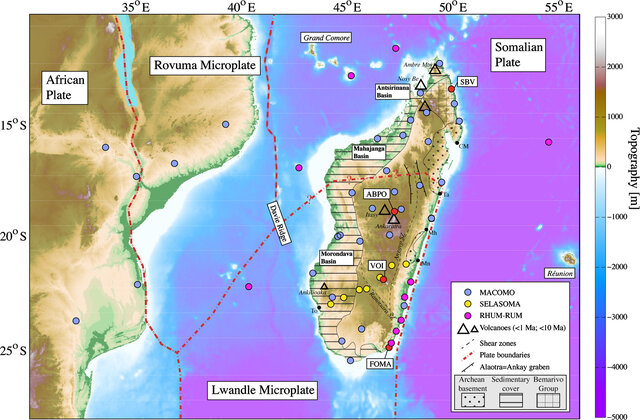
\includegraphics[width=0.5 \linewidth]{./geologyMadagascar.jpeg}
%     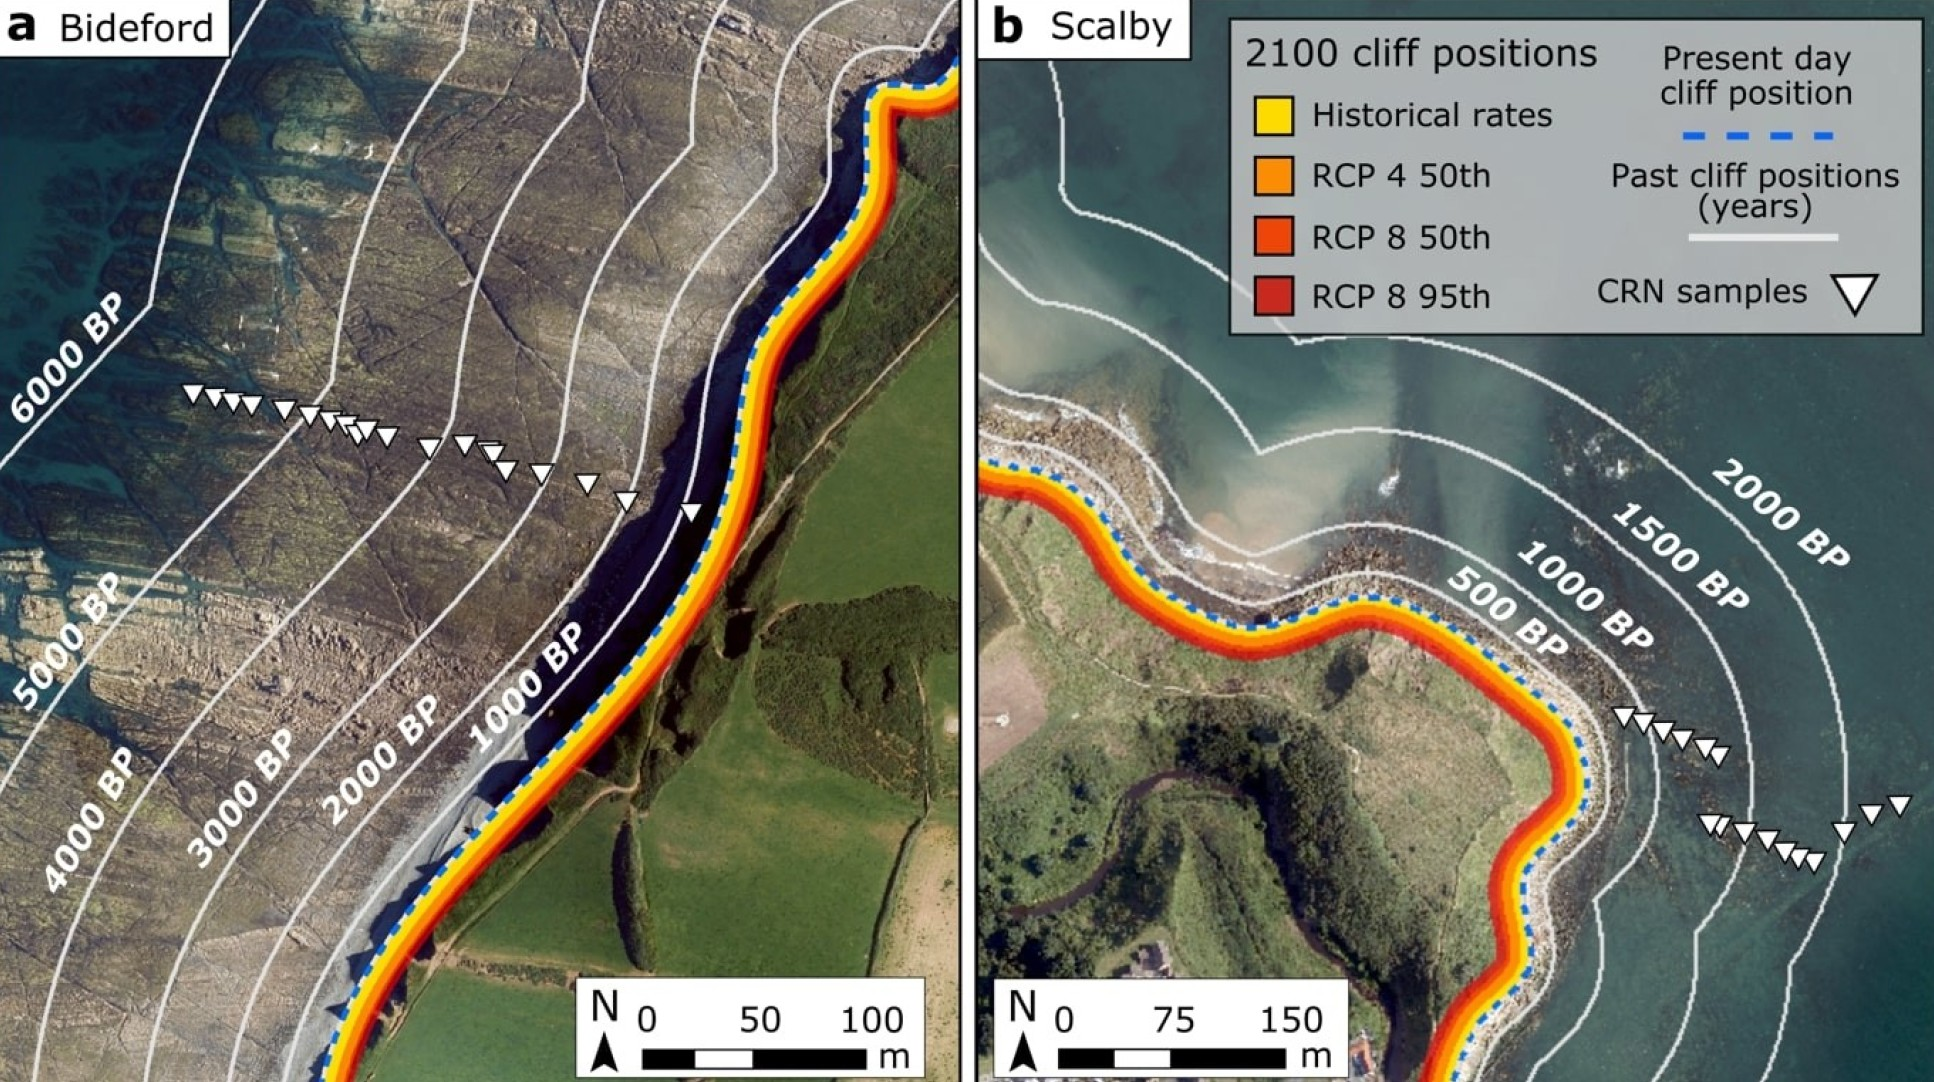
\includegraphics[width=0.5 \linewidth]{./CliffErosionBidefordAndScalby.jpg}
%     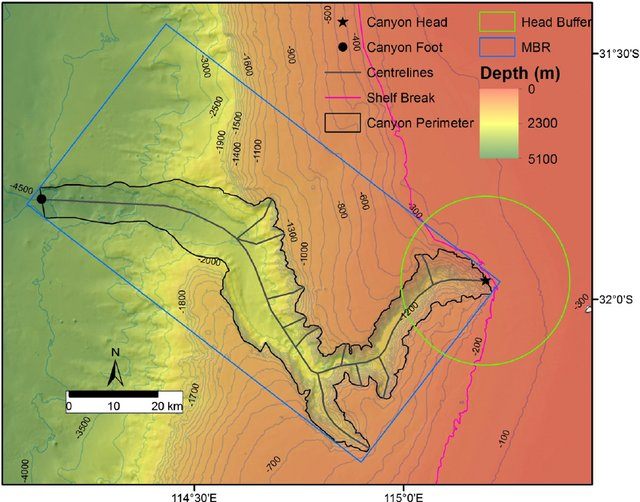
\includegraphics[width=0.5 \linewidth]{./PerthCanyon.jpg}
%     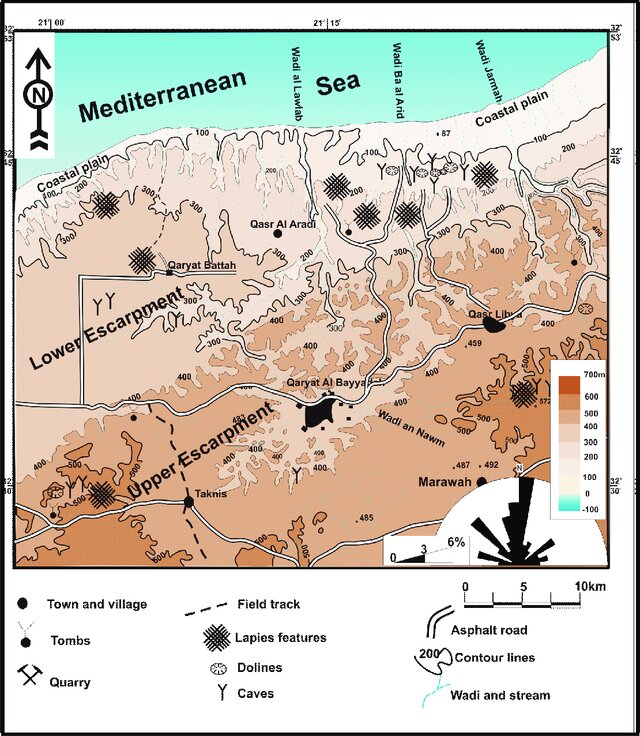
\includegraphics[width=0.5 \linewidth]{./QasrLibya.jpg}
%     \caption{Four examples of topographic maps used in earth science. From left to right and top to bottom: Sedimentary distribution other Madagascar island \cite{Pratt2017}, evolution of coastlines at Bideford, UK and Scalby, UK over the last 6000 years and 2000 years respectively (BP = Before Present) \cite{Shadrick2022}, localization of key parameters of Perth Submarine Canyon, Autralia \cite{Huang2014}, and geological features distribution of karstic landscape at Qasr Lybia, Libya \cite{ElAmawy2009}}
%     \label{fig:env-obj-presentation}
% \end{figure}

% Slight introduction
Topographic maps are very useful tools for biologists, geologists or even oceanologists (which would call them "bathymetric charts"). These maps are displayed in 2D but provide 3D information about the altitude (or depth), but can also use symbology to represent the elements of different scale order need to be visible for interpreting correctly the context of a map. In cartography, map symbols are defined as geometric primitives such as points, polylines, polygons, and (more rarely) polyhedrons. Map symbols are important in order to extract as much information as possible while being an extreme simplification of the content of an environment, or an abstraction of the 3D nature of the terrain features. 

This abstraction is useful to understand the relationship between the different features, which may enable to deduce physical rules in the evolution of a terrain through the process of observation. In fields where systemism is out of reach (earth science, biology, urbanism, ...), the deduction of rules through observation plays an important role in the understanding of phenomena and explication of situations. [A REDIRE VITE]

In such way, geologists can study the distribution of peaks in a mountain range, the location of soil types in an area (\cref{fig:env-obj-topo-madagascar}), which in turn allow to deduce possible locations of karst networks (\cref{fig:env-obj-topo-karst}), for example. Using the same abstraction tools, a biologist may interpret the effect of natural or artificial reefs on coastal erosion (\cref{fig:env-obj-topo-coasts}), or understand more clearly the interactions inside an ecosystem. Oceanologists may also deduce, using the same strategy, the formation of canyons and fans from old river systems (\cref{fig:env-obj-topo-canyon}). [A REDIRE]

\AltTextImageR{
The use of parametric lines representing coasts of islands or continents is heavily used as it is easy to understand the concept of interaction using curves. It also shows an easy way to present the evolution of this interaction with respect to time, as the continuous change of shape can be interpreted by our mind as a moving shape, providing a sense of velocity of change (\cref{fig:env-obj-topo-coasts}). While real coastlines are fractal, a representation using a continuous line is sufficient to be able to imagine the real scene. A complex representation would be, on the other hand, difficult to read, without any significant improvement on the possibility to understand the reality, harder to draw and edit, and much more subject to change with time and become obsolete.

Any element, like a coastline, then have an organic evolution over time, just like biologic elements as they can grow, shrink, and morph continuously. We see that one of the main differences of the evolution of organic elements, like the borders of a forest, and non-organic elements, like the borders of an island, reside in the time scale.
}{./CliffErosionBidefordAndScalby.jpg}{Evolution of coastlines at Bideford, UK and Scalby, UK over the last 6000 years and 2000 years respectively (BP = Before Present) \cite{Shadrick2022}}{fig:env-obj-topo-coasts}

\AltTextImageL{
Symbology can be used to represent at the same time large elements like regions with a specific type of soil, and very small and sparse elements like the peak of volcanos or buildings from \cref{fig:env-obj-topo-madagascar}. We can find, on a single map, elements described as 0D (sparse points, like volcanos and buildings), 1D (curves like the plate boundaries and shear zones) and 2D (regions like the sedimentary cover and tectonic plates).

The geometric shape used to describe an element may vary depending on the scale at which the topographist wishes to represent it, or depending on the work focus of the map. The observatories are presented as single points (0D) in an island-scale map, but could be found as regions (2D) on city-scale maps. Beaches may be represented as curves, points or regions if the objective is to present their distribution, position, or shapes.
}{./geologyMadagascar.jpeg}{Sedimentary distribution over Madagascar island \cite{Pratt2017}}{fig:env-obj-topo-madagascar}

\AltTextImageR{
A combination of multiple disciplines can be represented in a single topographic map to provide context about an area. We can find examples of representations with urbanism, geology, hydraulogy, and topography mixed together. Every discipline is linked with all others with relative strength. Urban regions are strongly affected by the geology and topography, while hydraulogy is directly impacted by topography. In this example, the karst geology is influenced by hydraulogy and geology, given that the presence of certain karst features are present in limestone areas with underground river networks. This also means that the presence of karst features can imply the presence (or a high probability of presence) of limestone and underground water flows, without the need to display them on a map. 

Without its 3D representation, a karst expert may be able to visualize in 3D from \cref{fig:env-obj-topo-karst} a possible ground surface around dolines and lapies without additional information.
}{./QasrLibya.jpg}{Geological features distribution of karstic landscape at Qasr Lybia, Libya \cite{ElAmawy2009}}{fig:env-obj-topo-karst}

\AltTextImageL{
The presence of symbols in a topographic map does not imply the presence of an element in the real world. We can commonly find indicative symbols like the head and foot of a canyon, or the area affected by an element, which have no real geometry. However, the presence of these symbols bring useful information. The head buffer displayed in \cref{fig:env-obj-topo-canyon} add an explication on the deformation of the shelf break line. Looking at it in the other direction, the deformation on the shelf break with the canyon implies the presence of a canyon head.
}{./PerthCanyon.jpg}{Localization of key parameters of Perth Submarine Canyon, Autralia \cite{Huang2014}}{fig:env-obj-topo-canyon}


Parallelly, terrain artists most of the time sketch the global shape of the terrain they will model beforehand, such that they can check, before the modeling part, that the consistency and plausibility of the terrain will be valid. Looking at a simplified map before starting the modeling step allows the designer to modify the overall shape of the terrain, at a large scale, before the 3D geometry comes into play, generating too much control points or vertices to be able to deal with. [TO CONTINUE]


As seen in the previous examples, by simplifying the surface details in maps or models we can concentrate more effectively on gaining a deep understanding of the underlying processes that shape the terrain. This focused understanding allows us to apply the insights we gain to a wide variety of terrain types. Essentially, this approach enables us to generalize our findings and apply them across diverse geographical landscapes, facilitating broader and more versatile applications of our knowledge.

In the use case of the generation of underwater environments, the elements to consider in a terrain vary greatly in size. Going from a single coral colony to a volcanic island, the use of topologic map enables biologists, geomorphologists, and hydrologists to study and understand the evolution of an area. The procedural construction of such landscape should fit the tools that the fields expert use in order to be coherent. 

The question which led to our solution is the multi-scale user interaction: "Is it possible to provide an interaction mean for terrain generation allowing the user to interact with a small structure like a rock in the same manner as with a large structure like a mountain?". 
In this work, we want the user to be able to have a large scale representation of the terrain in order to generate a landscape that satisfies his needs while keeping the possibility to apply large modifications.
In discussion with robotician users, we realise that we want to create a large landscape that can contain interesting configurations, select a smaller region that may have features in a disposition that fits its requirements and then refine again the given region.
In the optic of generating a large scale terrain in which we could focus the generation effort in a certain region, we wished to be able to see a coarse representation that can be computed quickly.

Starting from an initial configuration or providing conditions on the desired output terrain, the algorithm we propose will let the different terrain features evolve as a multi-agent system in which the user can apply modifications or new constraints on the state of the environment. The resulting configuration is an environment conform to the constraints given by the user over the distribution of features present in the scene.

We aim for our terrain generation method to be versatile enough to handle both terrestrial and aquatic environments. This dual capability would allow the method to be applicable to landscapes above the water level, such as mountains and valleys, as well as to submerged terrains, such as oceanic canyons and coral landscapes.

Because many geographical terms and computer science terms are deceptive cognates, we will try to find middle ground in the naming of our introduced structures to avoid as much as possible any ambiguity between the research fields.

\section{State of the art}
\label{sec:env-obj-related-works}

% Our work is highly ispired by the modeling of ecosystems, in which we consider abiological elements on the same level as biological organisms. 
Simulating ecosystems involves a range of modeling approaches, each balancing biological realism and computational efficiency. Broadly, models can treat populations as continuous fields using reaction-diffusion equations, or simulate each organism individually through agent-based methods. Site-based models discretize space to model local interactions efficiently. In contrast, individual-based models (IBMs) capture fine-scale behaviors and heterogeneity, often using spatial interaction rules like fixed-radius, zone of influence, or field-based methods. Ecological Field Models (EFMs) bridge these approaches by representing environmental properties as continuous fields influenced by organisms, enabling dynamic feedback between species and their surroundings. These diverse frameworks provide flexible tools for capturing complex ecological processes at varying scales and resolutions.

Our work aims to extend the Environmental Objects framework proposed by \citep{Grosbellet2016}, whose work is related to ecological fields. Bridging the gap between the ecological domain and graphics domain allows us to generalize the Environmental Objects to biologic and abiologic elements of an ecosystem by focusing the generation and simulation of scenes through the spectre of ecosystem services.

\subsection{Ecosystem simulation}

% Modeling of ecosystem extremely important in many fields. 

% Simulations study how a population grows and spread or moves over time. 

Two main philosophies can be extracted from the litterature: looking at population of species as continuous spaces, or studying each individual one by one \cite{Czaran1998}.

From a large scale observation, where billions of individuals are indicernable from one another (like grass sproot, bacteria, whole population, ...), we consider the species as a continuum and borrow diffusion-reaction models from physics and chemistry \cite{Turing1952}. 

On the other hand, when the number of individual becomes smaller or the density is low enough that we need to study individual one by one, the Individual-Based Models (IBM) become handy. This methods focus on the individuals as agents of a system, usually using sensing and interaction between agents to drive decisions, like spawning, growing and dying, in case of vegetation.

An hybrid method family, the ecological field models \cite{Wu1985}, proposed to describe how each individual modifies the state of its surrounding environment. These models represent the effect of each individual as spatial interferences, borrowing the field theory concept from physics. while itself being affected by the environment for decision making. Environment factors are intrinsicly includable in these models.

\subsubsection{Site-based models}

\begin{figure}[H]
    \centering
    % 
\includegraphics[]{placeholder.pdf}
    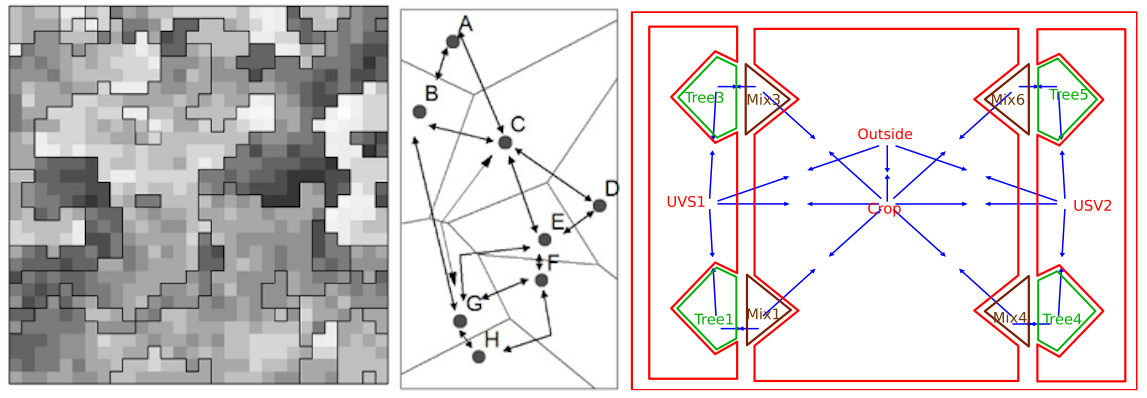
\includegraphics[width = .8 \linewidth]{grid-based-modeling-teaser.png}
    \caption{The grid-based models represent the environment as small discrete regions with uniform properties, providing interaction with each direct neighbors. This notion may be extended to regions organised in grid cells \cite{Nelson2012}, Voronoi cells \cite{Nelson2012}, or even generalized topological maps \cite{Lemiere2023}. }
    \label{fig:env-obj-grid-based-models}    
\end{figure}

\subsubsubsection{Grid-based models}
Grid-based models represent ecosystems by discretizing continuous space into a regular arrangement of cells, typically squares or rectangles, each containing uniform environmental properties and ecological conditions (\cref{fig:env-obj-grid-based-models}, left). In this approach, each cell represents a spatially explicit patch hosting one or multiple populations, with interactions primarily occurring between neighboring cells. The central ecological rationale for employing grid-based models is their conceptual simplicity, computational efficiency, and ease of representing spatial processes such as diffusion, dispersal, competition, or predation.

Mathematically, grid-based ecological dynamics are commonly described using discrete-time state equations that represent how the state of a cell (such as population density, biomass, or nutrient availability) changes according to its local interactions. A general formulation of these dynamics can be expressed as:
\begin{align}
    N_{t+1}(x,y) = f(N_t(x,y), \Bar{N}(x, y), E_t(x, y))
\end{align}
where $N_t(x, y)$ is the state variable ar cell coordinates $(x, y)$ at time $t$, $\Bar{N}(x, y)$ is the neighborhood of the cell at coordinates $(x, y)$, $E_t(x, y)$ is the explicit environmental factors like precipitation and soil nutrients, and $f$ is the update function that describe the biological changes given a current state, the neighborhood and the environment factors around a cell.

Grid-based models are particularly suited for simulations involving diffusion-like processes or phenomena with clear spatial boundaries. Classic examples in ecology include modeling vegetation dynamics in arid ecosystems, spatially explicit predator-prey interactions, forest-fire spread, and habitat fragmentation effects. Additionally, grid-based representations form the basis for Cellular Automata models, where cells exhibit discrete states (e.g., occupied, empty, burning), updated synchronously according to predefined state-transition rules.

Grid-based models are commonly used due to computational simplicity, easy integration with geographic information systems (GIS), and suitability for parallel computing. They facilitate large-scale ecological modeling by clearly defining spatial relationships and boundary conditions, thus making them practical for exploring broad-scale ecological hypotheses or management scenarios.

However, significant limitations exists as ecological processes may differ drastically at varying scales (e.g. local vs. landscape-level processes). Incorrect spatial resolution of the grid cells can lead to ecological inaccuracies or oversimplifications. Moreover, grid cells assume ecological homogeneity within each cell, which may poorly reflect natural ecological heterogeneity, especially in large cells. Complex ecological interactions, such as asymmetric competition or directional effects, are typically simplified or lost in grid-based discretization. Finally, regular grids impose artificial directional biases (e.g., horizontal/vertical) that can impact ecological interpretations, especially for processes that depend on continuous spatial gradients or isotropy.

\subsubsubsection{Tesselation models}
Tessellation models generalize the idea of grid-based approaches by partitioning continuous ecological space into discrete regions based on proximity rather than regular shapes (\cref{fig:env-obj-grid-based-models}, center). Among these methods, Voronoi diagrams (also known as Thiessen polygons in ecological studies) and their dual, Delaunay triangulations, are particularly relevant and widely applied.

Voronoi diagrams partition a plane based on a set of points (e.g., tree positions, animal territories, or resource centers). Each region in a Voronoi diagram is defined as the set of all points closer to a specific focal point (seed) than to any other point. Formally, given a set of points $\{p_1, p_2, ..., p_n\}$, the Voronoi region $V_i$ associated with the point $p_i$ is defined as:
\begin{align}
    V_i = \{ x \in \R^2 : d(x, p_i) \leq d(x, p_j), \forall j \neq i \}
\end{align}
with $d(x, p_i)$ the distance between the point $x$ and the seed $p_i$.

Conversely, the Delaunay triangulation is the dual graph structure of a Voronoi diagram. It connects points whose Voronoi regions share a common boundary, thereby explicitly defining neighborhoods among entities (e.g., individuals or resource patches). This duality between Voronoi and Delaunay representations provides two complementary perspectives: territorial partitioning (Voronoi) and direct adjacency or connectivity (Delaunay).

In ecological modeling, these tessellation methods have significant implications and applications. Voronoi diagrams naturally represent resource partitioning among individuals or populations, capturing territorial or competitive interactions without the artificial constraints imposed by fixed grids \cite{Castle2006}. For instance, they have been effectively employed in forest ecology to model individual-tree resource competition, where the area of a tree's Voronoi cell directly correlates to available resources and competitive interactions.

The use of tesselated models may become very useful as they adapt to irregular spatial distributions, accurately modeling ecological territories and resource accessibility based on actual entity locations.

They inherently define spatial neighborhoods without arbitrary distances or predefined shapes, enabling more precise representation of interactions among entities.

Unlike grids, Voronoi cells automatically adjust spatial resolution according to entity density, allowing finer resolution in densely populated areas and coarser resolution in sparse ones.

However, Voronoi-Delaunay models also present several limitations and challenges:
\begin{Itemize}
    \Item{} Dynamic updating of Voronoi diagrams and Delaunay triangulations is computationally more intensive than fixed-grid models, especially in large-scale or highly dynamic ecosystems where individuals frequently appear, disappear, or move.
    \Item{} Voronoi models implicitly assume isotropic interactions (competition or resource usage is equal in all directions) and strictly distance-based territories, neglecting directional biases like prevailing winds, slopes, or anisotropic resource gradients.
\end{Itemize}



% \subsubsubsection{Generalized topological maps}
Generalized topological maps represent ecosystems using abstract spatial relationships and connectivity structures, emphasizing the importance of spatial relationships or interactions rather than explicit geometric positions or shapes \cite{Urban2009}. Unlike grid-based or Voronoi-Delaunay tessellation models, generalized topological maps prioritize topological relationships over exact geometric distances or spatial coordinates (\cref{fig:env-obj-grid-based-models}, right). Formally, these maps can be defined as graphs or networks $G = (V, E)$, where vertices $V$ represent spatial entities (e.g., habitat patches, resources, individuals, or territories), and edges $E$ define ecological interactions, such as connectivity, dispersal pathways, competitive influence, or predator-prey relations \cite{Hamonic2021,Minor2008,Peterson2024}.

% In ecological modeling, generalized topological maps have notable advantages. 
By abstracting space into relational networks, these maps enable efficient representation and analysis of ecological processes in scenarios where exact geometry may be unknown, less relevant, or overly complex. They are particularly valuable in modeling metapopulation dynamics, habitat connectivity, or animal movement patterns, where the critical ecological factor is the presence or absence of connectivity rather than explicit spatial positions. Furthermore, generalized topological approaches facilitate integration with network theory, providing tools to analyze ecological resilience, robustness, fragmentation, and connectivity dynamics directly through graph-based metrics (e.g., connectivity indices, centrality measures, or modularity analyses) \cite{Lemiere2023,Gaucherel2012}.

However, the use of generalized topological maps also presents several limitations and ecological assumptions:
\begin{Itemize}
    \Item{} Removing explicit geometry sacrifices detailed spatial realism, potentially limiting the ability to accurately model distance-dependent ecological processes such as diffusion or continuous dispersal.
    \Item{} Ecological outcomes can be highly sensitive to how vertices and edges are defined, necessitating careful selection or validation of the underlying graph structure to avoid artificial ecological patterns or biased results.
    \Item{} Empirical calibration or validation may be difficult, as topological maps represent abstract ecological relationships rather than measurable spatial distances or tangible boundaries.
\end{Itemize}

Despite these limitations, generalized topological maps remain valuable tools, especially when combined with explicit spatial approaches \cite{Ecormier-Nocca2021} or when explicit geometry is unavailable or unneeded \cite{Duflot2018,Boussange2022}. 
% Examples of applications include modeling animal migration networks, habitat corridors, species dispersal networks, or the spread of invasive species through interconnected habitats.

% The grid-based models represent a density of a population in a discrete space. The interaction of each cell is usually limited to its direct neighbors.

% This models can be generalized to what could be called "Tesselation models", or "Site-based neighborhood models" \cite{Czaran1998}. The grid is a specialization with each region being a unit square sharing adjacency with its direct neighbors. However, the use of Voronoi diagrams (or "Thiessen polygon" in the biological field) and its duality, the Delaunay triangulation, may be used. As such, each vertex in the Delaunay graph is a small area with uniform properties and the influence between two regions is defined using the graphs edges. 

% The use of generalized topological maps furthermore dissociate the geometry to focus on the topological aspect of the ecosystem \cite{Lemiere2023}.

% Considering small regions to simulate the evolution of the ecosystem enables the use of cellular automata theory.

\subsubsection{Individual-based models}

\begin{figure}[H]
    \centering
    % 
\includegraphics[]{placeholder.pdf}
    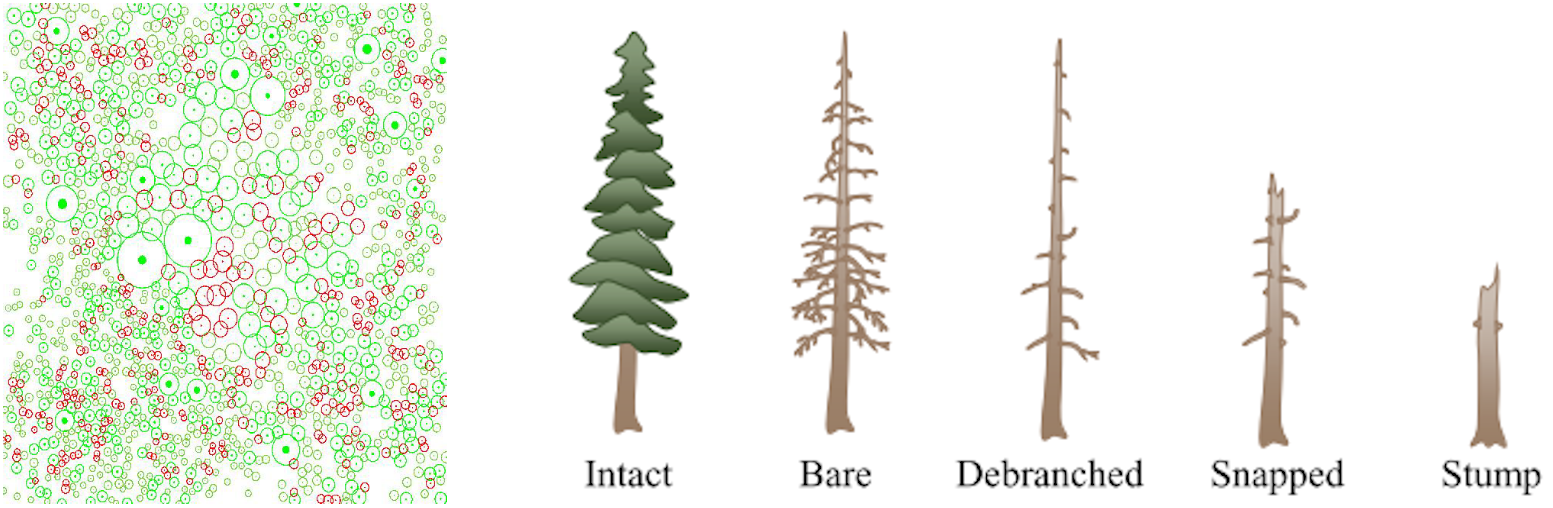
\includegraphics[]{individual-based-modeling-teaser.png}
    \caption{The individual-based models focus the attention on each element of the scene, with interaction with the neighboring entities. Choosing this point of view allows for more precision on the positionning of each tree \cite{Alsweis2006}, but also on the life cycle and geometry of the individuals \cite{Peytavie2024a}. }
    \label{fig:env-obj-individual-based-models}    
\end{figure}

In contrast to aggregated or spatially discrete models like grid-based and cellular automata methods, Individual-Based Models (IBM) explicitly represent each organism or ecological entity as a distinct unit \cite{Crooks2017}. Thanks to increased computational power, IBMs have gained popularity due to their ability to capture individual variability, spatial heterogeneity, and detailed ecological dynamics. In IBMs, each organism is modeled independently, enabling fine-grained representation of processes such as birth, growth, reproduction, mortality, dispersal, and competition, each potentially influenced by local environmental conditions or interactions with neighboring individuals \cite{Chng2013,Peytavie2024a}.

IBM inherently captures the variability and heterogeneity of natural ecosystems, thus providing ecological realism by explicitly modeling individual variability in life histories, behavior, and spatial positioning \cite{McLane2011,Zhang2020}. As such, IBMs are particularly effective for simulating complex ecological processes, including species interactions, competition, predation, dispersal, and responses to spatially heterogeneous environments  (\cref{fig:env-obj-individual-based-models}, right).

To reduce computational costs while maintaining ecological realism, IBMs frequently employ approximations such as distance-based competition methods (e.g., FRN, ZOI, FON), or stochastic processes capturing probabilistic interactions among individuals. Moreover, recent advances have improved the scalability and realism of IBMs by leveraging parallel computing and GPU-based simulations, facilitating large-scale applications.

Hybrid approaches are also common, combining IBM with grid-based or tessellation models to balance computational efficiency and ecological detail. Such hybrids may represent environmental conditions through spatial grids or tessellations (Voronoi diagrams) while explicitly modeling organism-level behaviors and interactions individually \cite{Chng2011a}.

% In opposition with the grid-based models, and in response to the increase of computer power, the research about ecosystem simulation leaned towards a new kind of model in which each individual of the system is represented independantly. The Individual-Based Models (IBM) sees each element of the system as an entity that spawn, grow, die, and possibly transport itself depending on its surroundings. 

% In order to simulate ecosystems with these models, the behaviour of single individuals with respect to the environment properties must be modeled. The main environmental factor being sunlight, the exact computation of shading for estimating the rate of growth of trees was expensive without the use of parallel computing and the use of GPU. In response to this constraint, the most common approximations accepted are "distance-based models". 

\subsubsubsection{Fixed-Radius Neighborhood}
In the Fixed-Radius Neighborhood (FRN) method, the first appearance of a distance-based method, each tree has a radius inside which we consider that there is shade and competition of nutrients. It two trees' radii intersect, a competition let the strongest tree live while the weakest die (\cref{fig:env-obj-individual-based-models}, left). 

\AltTextImage{

    The computer graphics community represents the FRN constraint by using Poisson Disk Sampling or blue noise approximations \cite{Deussen2000} to generate entities as points that does not fall inside any other radius. The algorithm can be accelerated by using a regular grid structure as proposed by \citep{Bridson2007b}: each cell of the grid has a width of $\frac{\radius}{\sqrt{n}}$ with $n$ the number of dimensions (usually $n = 2$). Each point sampled is encoded by the grid cell in which it resides. A cell can only contain a unique point, making it a fast spatial structure for distance computation with other points. Each point added in the grid recursively instantiate new random samples in a spherical annulus of between radius $\radius$ and $2 \radius$. While this method is fast and simple, other methods propose variations on it to add the guarantee of maximal coverage \cite{Ebeida2011} or GPU parallelisation \cite{Wei2008}. However, in the presence of at least two species of different radius, the circle packing problem becomes more complicated and require a larger amount of collision detection, while keeping the spatial indexing method from Bridson's algorithm.

}{Poisson_disk_sampling.png}{Poisson Disk Sampling iteratively add points in space and checks whether the new points fall inside one of the previously instanciated points and radii. }{fig:env-obj-poisson-example}

\subsubsubsection{Zone of Influence}
\AltTextImage{

    The Zone of Influence (ZOI) model is an ecological method designed to quantify competition among trees by modeling their interactions as gradual rather than binary processes \cite{Czaran1998}. In contrast to simpler binary approaches such as Fixed Radius Neighborhood (FRN), the ZOI model assigns each tree a circular influence zone, typically defined based on measurable attributes like diameter at breast height (DBH), crown dimensions, or species-specific ecological characteristics.

    In this framework, competition between adjacent trees is quantified by calculating the fractional overlap between their influence zones (visible in \cref{fig:env-obj-zoi-scheme}). 

    }{ZOI-Peters2020.png}{ZOI is represented by regions around entities. The intersection between two circular regions (radii) define the competion between the two entities \hide{ (from \cite{Peters2020})}}{fig:env-obj-zoi-scheme}

Mathematically, the intensity of competition $C_{ij}$ exerted by a neighboring tree $j$ on a focal tree $i$ is expressed as:
\begin{align}
    C_{ij} = \frac{ \Area_{\text{overlap}, ij} }{ \Area_{\text{ZOI}, i} }
\end{align}
where $\Area_{\text{overlap}, ij}$ is the area of overlap between the radii of trees $i$ and $j$, and $\Area_{\text{ZOI}, i}$ is the total area of the influence zone of tree $i$. This intersection area can be computed directly with:
\begin{align}
    \Area_{\text{overlap}, ij} = &r_i^2 cos^{-1}\left( \frac{d^2 + r_i^2 - r_j^2}{2 d r_i} \right) + r_j^2 cos^{-1} \left(\frac{d^2 + r_j^2 - r_i^2}{2 d r_j} \right) \nonumber \\
    & - \frac{1}{2} \sqrt{(-d + r_i + r_j)(d + r_i - r_j)(d - r_i + r_j)(d + r_i + r_j)}
\end{align}
assuming $r_i$ and $r_j$ the radii of trees $i$ and $j$ respectively and $d$ the distance between the two centers.

The biological consequences of competition quantified by ZOI, such as reduced growth or increased mortality risk, can be represented through growth-response equations. For instance, tree growth under competition might be modeled as \cite{Das2012,Uriarte2004}:
\begin{align}
    G_i = G_{\text{max}, i} \left(1 - \alpha \sum_{j} {C_{ij}} \right)
\end{align}
with $G_i$ the growth of the tree and $G_{\text{max}, i}$ the maximal potential growth if no competition affect it, and $\alpha$ a sensitivity parameter determining how competition affect the tree growth.


\AltTextImage{

    The ZOI model typically assumes symmetric (isotropic) competition, meaning all trees compete equally in every direction, and the competition effect between two trees is reciprocal if their zones and dimensions are similar. However, ecological realism can be increased by adopting an asymmetric (anisotropic) version of the model, which acknowledges that competition is often directionally biased or size-dependent. For asymmetric competition, the equation is modified by introducing weighting based on differences in tree size or dominance, for example:
    \begin{align}
        C_{ij} = \frac{ \Area_{\text{overlap}, ij} }{ \Area_{\text{ZOI}, i} } f(DBH_i, DBH_j)
    \end{align}
    with $f(DBH_i, DBH_j)$ a function that introduce asymmetry due to a difference in the diameter at breast height (DBH) of the two different trees, modeling the stronger drainage of resources by larger trees, or using $f(h_i, h_j)$ to add model light competition between trees with different heights.
    
}{FON-asymmetric-field-Peters2020.png}{The main inconvenient of methods using individual-based models is that the influence of each entity is supposed isotropic, without taking into account the environmental factors. (from \cite{Peters2020}) }{fig:env-obj-fon-asymmetric-scheme}

The ZOI model is theoretically rooted in the understanding that trees compete gradually and continuously, rather than abruptly. However, it does rely on simplifying assumptions, such as circular, isotropic zones, homogeneous environmental conditions, and static radii within measurement intervals, which can limit its applicability to certain ecological scenarios involving directional resource gradients or heterogeneous environments.

Empirical studies across diverse forest ecosystems have demonstrated that the ZOI approach significantly improves predictions of tree growth, survival, and mortality compared to simpler binary models like FRN. The nuanced representation of competition offered by ZOI models better captures complex ecological dynamics, particularly in mixed-species stands, uneven-aged forests, or structurally diverse ecosystems.

\subsubsubsection{Field Of Neighborhood}

\AltTextImage{

    The Field of Neighborhood (FON) approach provides an alternative method to quantify tree competition by explicitly incorporating distance-dependent and size-dependent effects of neighboring trees on a focal tree's growth or survival \cite{Berger2000}. Unlike the ZOI model, which uses circular zones and geometric overlaps, FON models typically rely on explicit indices that incorporate both the distance and the relative sizes of neighboring trees, without necessarily defining explicit geometric overlap areas.

    In the FON approach, competition intensity affecting a given focal tree is calculated by summing the competitive effects of neighboring trees, typically as a weighted function of their size and distance. 
}{FON-Peters2020.png}{The FON model proposed a smoother version of the ZOI, such that the intersection between the two radii also take into account the distance from the tree trunk. (from \cite{Peters2020})}{fig:env-obj-fon-scheme}

A commonly used formulation of competition intensity $FON_i$ for a tree $i$ at the distance $r$ from the trunk is expressed as 
\begin{align}
    FON_i(r) = \begin{dcases}
        1 & \text{for } 0 \leq r < \text{RBH}, \\
        e^{-c(r - \text{RBH})} & \text{for } \text{RBH} \leq r \leq R, \\
        0 & \text{otherwise}
    \end{dcases}
\end{align}
with RBH the radius at breast height (half of the DBH) and $R$ the radius of influence of the tree (usually proposed to be $R = a \sqrt{\text{RBH}}$ given a scaling parameter $a$) and $c$ an attenuation coefficient, defined for each species. 


\AltTextImage{
    The overall competition at any point of space may now be described as:
    \begin{align}
        F(x, y) = \sum_{i} {FON_i(x, y)}
    \end{align}

    Now the competition percieved by a tree $i$ is the average of all $FON$ around its area $A$ (and symbolising $A' = \Area_{\text{overlap}, ij}$):
    \begin{align}
        F_A^i = \frac{1}{A} \sum_{j \neq i}{ \int_{A'}{FON_j(x, y) \, da'} }
    \end{align}

}{FON-scheme-Berger2000.png}{The evaluation of the FON value at any point is the simple accumulation of individual fields.}{fig:env-obj-fon-compute-scheme}
Unlike the ZOI method, the FON model does not assume a hard boundary around each tree, instead explicitly capturing a smooth decline in competitive impact with increasing distance. It also inherently accommodates asymmetric competition, since larger and closer neighbors exert disproportionately stronger competitive influences than smaller or more distant trees.

The FON method does not rely explicitly on geometric overlap and is thus flexible and particularly useful in heterogeneous forests. However, in order to capture the self-thinning property of silviculture \cite{Makowski2019} satisfying $ W = c N^{-\frac{3}{2}} $ (with $W$ the average biomass of an individual, $N$ the density and $c$ a constant) \cite{Westoby1984}, the generation of the ecosystem should be iteratively simulated with small time steps \cite{Alsweis2005}, which is computationally expensive. Instead of simulating the full growth model of vegetation, most ecosystem generation algorithms focus on the distribution of the elements of the terrain, abstracting the competion into distance function deformations or statistical optimization. 

\AltTextImage{
    By designing non-monotonous field functions around trees, an emergence of different behaviour can appear. \cite{Lane2002} proposed to apply a "deformation kernel" on the distance function, resulting in a larger variety of patterns like the clustering of bushes and the competition of larger trees (\cref{fig:env-obj-kernels-Lane2002}, top left). From this idea, the definition of deformation kernels for each pair of species (\cref{fig:env-obj-kernels-Lane2002}, top right, with kernels for two species) allows the system to include the ecological interaction between the different species in the terrain. As a result, the simulation of the ecosystem can introduce intra-species clumping while keeping inter-species segregation.

}{kernel-matrices-Lane2002.png}{The deformation of neighborhood kernels enables the modelling of different behaviour for species and inter-species interactions}{fig:env-obj-kernels-Lane2002}

\AltTextImage{
    On the other hand, learning the spatial distribution of distances between individuals from examples can be used as a statistical metric to introduce interactive tools for ecosystem generation \citep{Emilien2015a}. In this work, given a user-provided example, the system learns the parameters such as the histogram of distances inter- and intra-species from one region and reproduce these distribution in another regions. This method then does not limit to trees, but may include any scene element like houses and roads, as well as the integration of other metrics than distances such as the terrain slope.
}{worldbrush-Emilien2015.png}{Using statistical distribution from an input terrain, \cite{Emilien2015a} resynthesize a different terrain with similar distributions. }{fig:env-obj-worldbrush-Emilien2015}

While the FON model provides a biologically detailed representation of competition, its computational complexity makes it significantly more challenging to implement in large-scale simulations. Unlike the ZOI model, which relies on predefined geometric overlaps that can be calculated efficiently, the FON approach requires integrating a continuously decaying competition function over an arbitrary area of influence. This necessitates evaluating the function at multiple points across overlapping zones, increasing computational demand. Moreover, the additive nature of FON, where each tree contributes to the total competition field at every spatial point, further exacerbates the cost, scaling poorly in dense forest stands. The necessity of numerical integration or spatial discretization makes FON computationally expensive compared to ZOI, which only requires simple geometric calculations. Consequently, while FON is useful for small-scale or highly detailed ecological studies, it is generally impractical for large-scale forest simulations.



% To address these challenges, computational approximations such as discretized grids, kernel density estimations, or hybrid models combining FON for local interactions and ZOI for broader simulations may offer viable alternatives. Nonetheless, ZOI remains the preferred approach for efficiency and scalability in large-scale forest dynamics modeling.

% However, the FON model also has assumptions and limitations: notably, it assumes the effects of neighbors accumulate additively, often ignoring possible interactive or nonlinear competition effects, and typically relies on empirically tuning the $FON_i$ functions, which require extensive field data for accurate calibration.
% Introducing kernel functions instead of binary radii, representing a distance weight around each tree allows two radii to overlap without having to remove an entity, and even consider a different kernel for different pairs of species (see: a tree-tree kernel is highly different than a bush-tree kernel). Another advantage of the introduction of a kernel is to simulate multiple factors at once, like the importance of roots, the shade provide, the drainage of water, etc... \cite{Berger2000} This Field of Neighborhood (FON) method is a generalisation of the Fixed-Radius Neighborhood method since the later is simply the use of binary kernels for each tree.




\subsubsection{Ecological Field models}

\begin{figure}[H]
    \centering
    \autofitgraphics[width = .8\linewidth]{ecological-fields-example-shade-Wu1985.png, ecological-fields-example-water-Wu1985.png, ecological-fields-example-nutrients-Wu1985.png}
    % 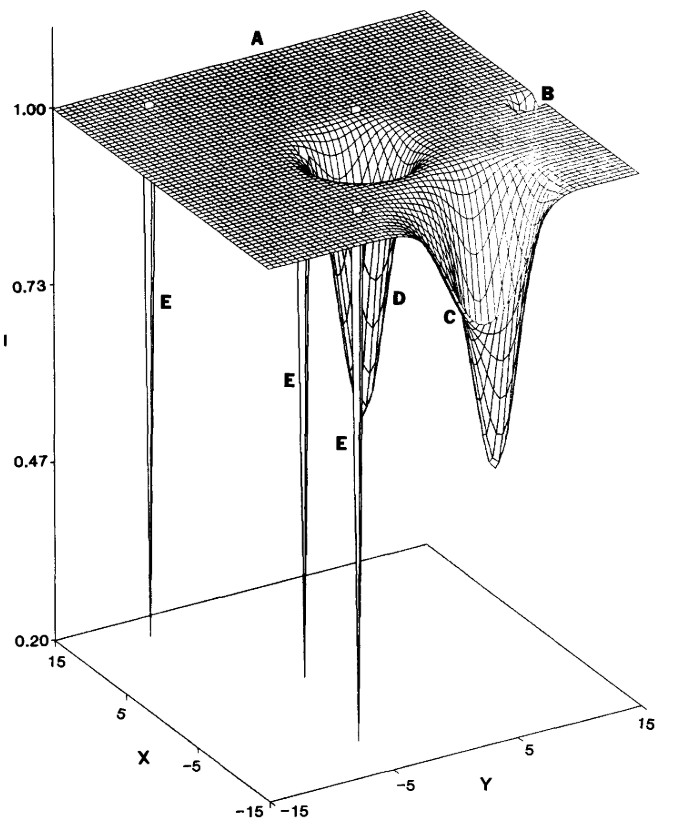
\includegraphics[width = .25 \linewidth]{ecological-fields-example-shade-Wu1985.png}
    % 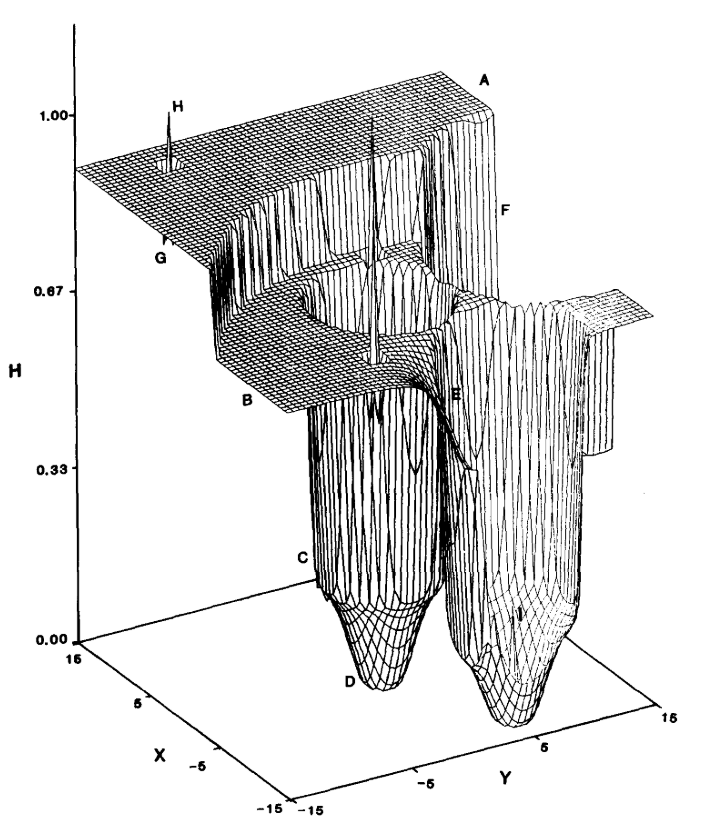
\includegraphics[width = .25 \linewidth]{ecological-fields-example-water-Wu1985.png}
    % 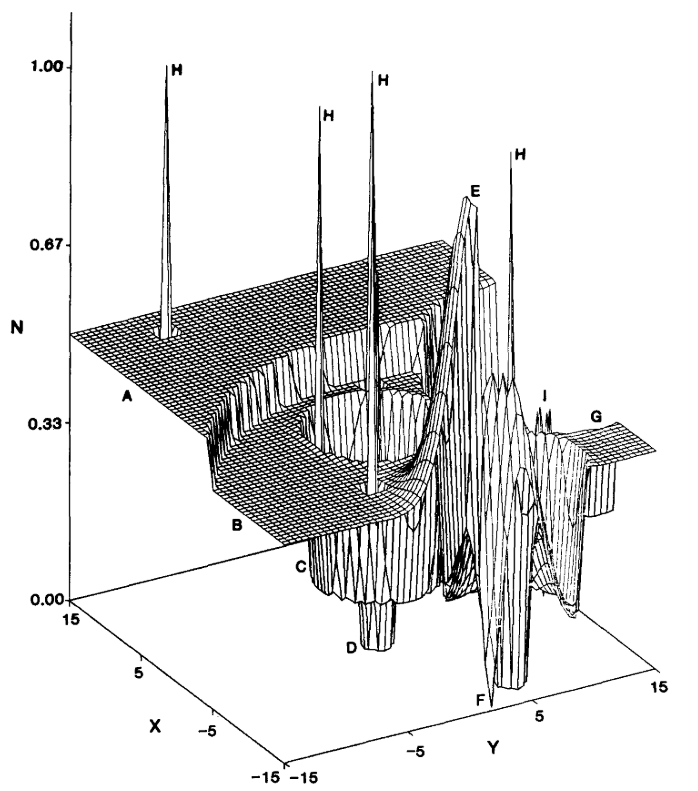
\includegraphics[width = .25 \linewidth]{ecological-fields-example-nutrients-Wu1985.png}
    \caption{Ecological Field models represents the environment as a mathematical function where environmental properties like humidity, shade and nutrients are seen as distinct fields (in the figure, respectively from left to right). }
    \label{fig:env-obj-ecological-field-models}    
\end{figure}

Modeling ecosystems requires a careful balance between biological realism and computational efficiency, especially when simulating large-scale environments. Traditional ecological models fall into two primary categories: Site-Based Models and Individual-Based Models, each with distinct advantages and limitations.

Site-Based Models discretize the environment into discrete regions, making them efficient for large-scale simulations but limited in their ability to represent smooth, continuous interactions. On the other hand, Individual-Based Models explicitly simulate each organism as an independent entity, allowing for detailed biological behavior and interactions, but quickly becoming computationally expensive when dealing with large populations.

While these approaches have been successfully used in various ecological studies, many real-world ecological processes do not fit neatly into a discrete grid or a set of independent agents. Instead, they operate in a continuous spatial domain, where organisms interact with smooth environmental gradients rather than discrete neighbors. For example, the competition for light and nutrients is not limited to the direct neighbors.

To address these challenges, Ecological Field Models (EFMs) provide an alternative framework where environmental properties are represented as continuous spatially explicit fields \cite{Wu1985}. Rather than defining interactions through direct contact (as in IBMs) or discrete adjacency (as in SBMs), EFMs describe how organisms modify and respond to smooth environmental gradients \cite{Chng2011b,Seidl2012}.

From a computer graphics perspective, EFMs share similarities with techniques used in Signed Distance Fields (SDFs). Just as SDFs encode geometric influences in a continuous field, EFMs encode ecological influences, allowing for more realistic ecosystem simulations.

EFMs are based on the fundamental idea that organisms are not isolated agents but rather integral components of their environment, influencing and being influenced by it in a spatially explicit manner. The core ecological principles behind EFMs include two keypoints:
\begin{Itemize}
    \Item{The continuous organism-environment interactions:} Organisms modify their surroundings in ways that extend beyond their immediate location.    Environmental factors such as soil nutrients, water availability, light exposure, and chemical signals influence other species gradually across space.
    \Item{The environmental fields influence the organism's growth and behaviour:} Species respond to spatially varying gradients rather than direct neighbor-based interactions, which we can see with phototropism guiding the growth of plants towards higher light availability areas \cite{Pirk2012} or the foraging strategy that develop roots of trees toward nutrient-rich soils \cite{Li2023}. 
\end{Itemize}

The combination of these two principles creates naturally feedback loops that are explicitly modeled, allowing a more realistic representation of ecological interactions compared to static environmental assumptions in traditional models.





EFMs provide a continuous representation of environmental factors, bridging the gap between grid-based and individual-based models by modeling smooth ecological gradients, instead of forcing interactions into discrete cells. This method allows organisms to influence and respond to fields dynamically, while providing a scalable framework that avoids the computational explosion of tracking every individual separately.


While EFMs provide a biologically grounded approach to modeling spatial interactions, their implementation requires a robust mathematical framework to define how organisms modify and respond to environmental fields. 





An ecological field represents a spatially varying environmental property across a landscape. Mathematically, we can define a $n$-dimensional ecological field as a scalar field:
\begin{align}
    F(\p) : \R^n \to \R
\end{align}

Any organism in the scene has an influence on the ecological fields through "influence functions" $K$. These functions describe how an organism's presence affects its surroundings. We can then evaluate the ecological field with $N$ entities:
\begin{align}
    \label{eq:env-obj-eco-field-computation}
    F(\p) = F_0(\p) + \sum_{i=0}^{N}{K_i(\p)} 
\end{align}
with $F_0(\p)$ the baseline environmental state.




The primary challenge in computer graphics is how to efficiently store, sample, and modify continuous environmental fields. Since EFMs define spatially varying properties, they require a structured representation that balances accuracy, efficiency, and scalability.

Several methods exist for implementing spatially explicit fields in graphics:
\begin{Itemize}
    \Item{} A common approach is to discretize the environment into a regular 2D or 3D grid, where each cell stores a value corresponding to an ecological property, such as soil moisture, nutrient concentration, or shading intensity. This approach has the advantage of efficient lookup and updates, and GPU compatibility at the cost of memory usage and precision loss. 

    \Item{} Rather than storing explicit values at discrete locations, ecological fields can be defined using procedural functions that are evaluated dynamically. This approach is particularly relevant in procedural terrain and vegetation generation, where continuous field functions determine environmental parameters. A Signed Distance Field (SDF), frequently used in raymarching and volumetric rendering, can be adapted for EFMs by encoding environmental influence functions. This approach enables a theoretical infinite precision for a compact memory footprint at the expense of high computational demand.
\end{Itemize}



\subsubsubsection{Environmental Objects}

\begin{figure}[H]
    \centering
    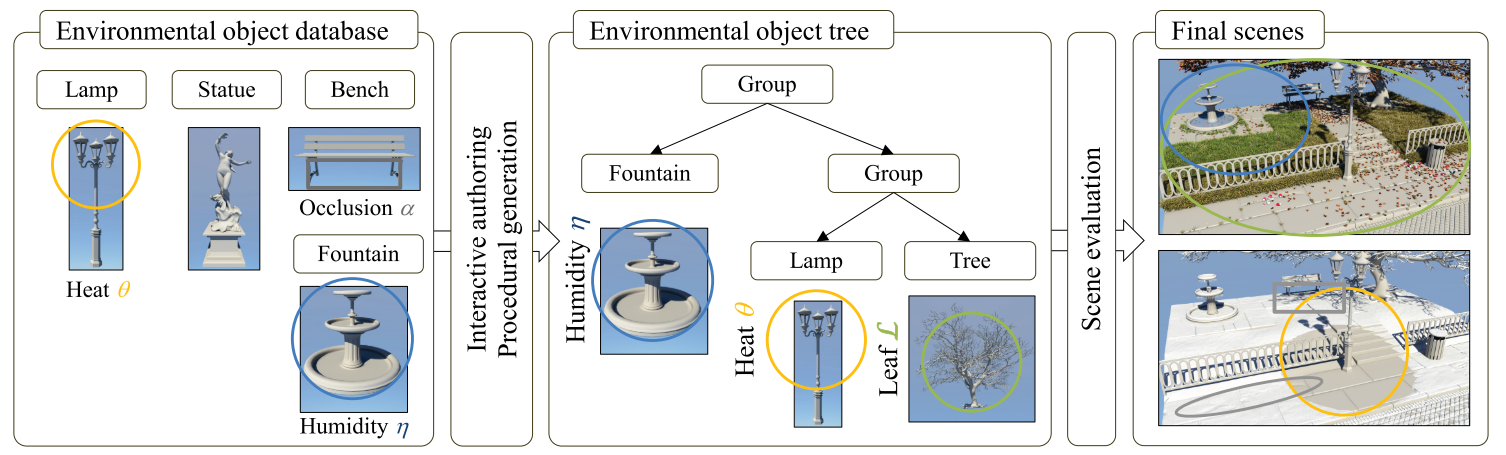
\includegraphics[width = .8 \linewidth]{env-objs-Grosbellet2016.png}
    \caption{The Environmental Objects framework \cite{Grosbellet2016} presents a practical methodology for integrating spatially explicit environmental interactions into procedural modeling. The Environmental Objects concept aligns closely with EFMs, providing a computationally feasible way to embed field interactions into simulated ecosystems.}
    \label{fig:env-obj-teaser-grosbellet2016}
\end{figure}

\citep{Grosbellet2016} proposed an application of Ecological Fields for the generation of outdoor scenes by associating the elements of the scene to scalar fields representing, for example, humidity, occlusion, heat, or even leaves fields. The presence of these fields allows each object to modify their geometry in order to integrate chages such as the deposition of snow, icicles, leaves piles, or grass. 

Despite its origins in computer graphics, this model shares conceptual similarities with EFM, which describes how spatially distributed ecological influences shape organism behavior and ecosystem dynamics. EFM operates within the domain of spatial ecology, defining ecological fields that influence species distributions and interactions. While these models have distinct applications, they both employ spatially explicit field-based approaches to describe how entities interact with their environment.


The Environmental Objects' method presents a hierarchical framework for authoring procedural scenes by extending objects (assets) with environmental fields that control their appearance and interaction with the virtual environment (\cref{fig:env-obj-teaser-grosbellet2016}). This work tackle the main problem with the modeling an urban scene, which is finding a balance between generating and editing a large scene in interactive time and the integration of small-scale details in coherence with the global environment: 
\begin{Itemize}
    \Item{} Objects in a virtual scene dynamically adjust their appearance based on surrounding scalar fields, allowing for realistic procedural effects such as snow deposition, leaf accumulation, and icicle formation. Unlike global simulations, which are computationally demanding, this model uses local environmental fields to procedurally generate details without requiring extensive physics-based calculations.
    \Item{} Users can modify environmental parameters, such as temperature fields, to influence scene aesthetics in an intuitive and predictable manner. The model enables scene composition through level of details using object groupings, optimizing the computation of large-scale environments while maintaining local control over environmental interactions.
\end{Itemize}
By employing skeletal implicit primitives and procedural blending techniques, the framework enables the efficient simulation of environmental changes while allowing for real-time scene modifications. 

In this method, each 3D model can be associated with "procedural effects", which regroup scalar fields representing changes in the environment. These fields are defined using skeleton-based implicit primitives, allowing to change the environment properties along a path instead of only using points like the initial EFM. This enables the system to represent for example the diffusion of heat around a pipe, which is not possible with the later. The computation of an environment property is then an agglomeration of all the scalar fields associated to the given property. The authors propose to compute the all scalar fields, like the heat field $\theta$, at any position $\p$ by the accumulation of objects' fields, in a similar manner as \cref{eq:env-obj-eco-field-computation}: 
\begin{align}
    \theta(\p) = \theta_0(\p) + \sum_{i=1}^{n}{ \theta_i(\p)}
\end{align}
and the occlusion field $\alpha$ as the product of all objects' occlusion fields:
\begin{align}
    \alpha(\p) = \alpha_0(\p) \prod_{i=1}^{n}{\alpha_i(\p)}
\end{align}
assuming $\theta_0$ and $\alpha_0$ to be global scalar fields for temperature and shade, symbolising the baseline environmental state in the ecological domain.

\AltTextImage{
    Using the field values, the system instantiates small details like leaves by sampling the space with candidate "anchor positions". If the field values satisfy certain conditions at the anchor position $\p_i$, the small scale objects can be instantiated at this position (for example, for leaves: $\alpha(\p_i) l(\p_i) < d_i$ using the occlusion field $\alpha$, the leaves deposition field $l$ and the distance of the anchor position to the depositing surface $d_i$). This method can then be easily extended to modify the geometry or texture of the object based on the field values like the heat field or the humidity field, to manually move or rotate each of the objects, or even integrate user-defined density fields to populate entangled details on the ground \cite{Guerin2016}. 
}{EnvObjs-leaves-instances-Grosbellet2016.png}{Leaves are instanced if the fields are sufficient and the geometry and texture are altered depending on the environment}{fig:env-obj-leaves-instances}

\AltTextImage{
    On the other hand, the geometry of large objects can be altered using the scalar fields. The authors present a simulation of snow deposition on the objects by displacing the vertices $i$ in the direction of the normals $\vec n_i$ by an amount depending on the environment:
    \begin{align}
        \p_i' = \p_i + \left( \alpha(\p_i) s(\p_i) g(d(\p_i)) - \theta(\p_i) \right) \vec n_i
    \end{align}
    with $s$ the "snow field", and $g$ a snow elevation function based on the distance between the original vertex and the border of the mesh.
}{EnvObjs-snow-Grosbellet2016.png}{Snow deposition is a displacement of vertices along the normals of the mesh}{fig:env-obj-snow-Grosbellet2016}

\AltTextImage{
    In addition to the EFM framework, the environmental effects from environmental objects are not limited by points geometry as the scalar functions may use a spline primitive or be extended to volume primitives. Translated to the ecological domain, this methodology extends the EFM as the inclusion of water bodies, essential for realistic vegetation simulation, can be taken into account by considering environmental effects from rivers and lakes which are often modeled as splines and regions in 3D modeling \cite{Emilien2015,Genevaux2013,Genevaux2015}.
}{env-obj-fields-heat-Grosbellet2016.png}{The heat field produced by a pipe uses a distance function from a line instead than a single point in space.}{fig:env-obj-heat-field-effect}

The Environmental Objects method can be seen as a variant of the EFM due to their high reliance on the idea of fields and environmental effects of each element on the environment, even if the purposes of each method are opposed: one tend to model the environment properties given the elements present while the other aims at altering the geometry of a scene given the elements in the scene, regardless to their biological nature. However, the convergence of these approaches suggests possibilities for cross-disciplinary innovation. The integration of ecological dynamics into procedural modeling could lead to more adaptive virtual environments that respond realistically to environmental changes, while procedural techniques could enhance ecological simulations by improving scalability and visualization.

The conceptual parallels between these models suggest potential areas for cross-disciplinary application. Insights from EFM could inform procedural content generation, enabling more realistic and adaptive virtual ecosystems by incorporating agent-based dynamics, ecosystem succession models, and time-dependent environmental changes. Conversely, procedural modeling techniques from computer graphics could enhance ecological simulations, improving visualization, scalability, and user interactivity in landscape ecology and biodiversity modeling. 


% Modern application of EFM include the notion of diffusion in order to depict the dynamic evolution of nutrients with respect to external boundaries such as a scene with different soil porosity or topography. 

The original EFMs work effectively for static environmental conditions, but many real-world ecological processes involve dynamic, time-dependent changes. For instance, soil moisture depletes over time, plant growth alters shading conditions, and chemical scent trails decay. By integrating biologically inspired feedback loops, procedural generation could extend beyond static environmental effects, enabling simulations of growth, decay, and species interactions \cite{Okubo2001,Wojtek2022}. To extend Environmental Objects beyond static environmental representations, we turn to reaction-diffusion models, which provide a mathematical foundation for modeling time-dependent field interactions used in ecological simulations. 




















% Although Grosbellet et al.’s procedural model was developed within the domain of computer graphics, it shares significant conceptual similarities with Wu’s Ecological Fields Model (1985). Wu’s framework describes ecological fields as spatially distributed influences that govern organismal interactions with their environment, shaping patterns of species distribution and community dynamics. In this approach, organisms respond to variations in ecological fields, which can represent factors such as resource availability, competition, and environmental constraints.

% Similarly, Grosbellet et al. employ scalar fields to define environmental influences on objects within a virtual scene. These fields dictate changes in appearance, determining the extent of environmental effects such as the accumulation of snow, the growth of grass, or the placement of fallen leaves. The fields act as local, distributed parameters that influence an object’s properties based on its surroundings. Both models conceptualize their respective domains in terms of spatial gradients, emphasizing how entities whether living organisms or computer-generated objects are influenced by their spatial context.

% Another point of similarity between the two models is their hierarchical structure. Wu’s model applies to multiple scales of ecological organization, ranging from individual organisms to entire ecosystems. It accounts for local-level interactions, such as how an individual plant experiences resource competition, while also considering broader landscape-scale patterns. Similarly, Grosbellet et al.’s procedural framework structures virtual environments using a hierarchical composition of environmental objects. These objects can be grouped together to optimize computation, and the influence of environmental fields can be controlled at various levels of the hierarchy. This allows for efficient and scalable scene generation while maintaining fine control over localized details.

% Despite these similarities, the models differ in their intended applications. Wu’s framework is designed for ecological analysis and predictive modeling, aiming to describe and explain real-world ecological patterns. In contrast, Grosbellet et al.’s model is intended for aesthetic and interactive purposes within computer graphics, focusing on visual realism and user control rather than ecological accuracy. Nevertheless, both models offer a field-based perspective on how spatially distributed influences shape system-level outcomes, making them conceptually related despite their distinct disciplinary origins.


% The fundamental similarity between Wu’s Ecological Fields Model and Grosbellet et al.’s procedural modeling framework lies in their shared reliance on spatially distributed fields as a mechanism for mediating interactions. Both models define spatial gradients that influence entities within an environment, allowing for context-dependent interactions. In Wu’s framework, organisms respond dynamically to environmental gradients, which may influence their movement, resource consumption, and reproductive success. Similarly, in Grosbellet et al.’s model, objects within a virtual scene react to environmental scalar fields, altering their appearance in response to predefined environmental conditions such as temperature and humidity.

% Despite this shared structural foundation, the two models differ significantly in their underlying mathematical formulations and computational implementations. Wu’s model is rooted in ecological theory and often employs differential equations and statistical spatial models to describe species-environment interactions. These methods allow for the prediction of ecological dynamics over time, incorporating feedback mechanisms and stochastic variation. In contrast, Grosbellet et al. utilize procedural techniques, such as skeletal implicit primitives and rule-based field blending, to generate visually plausible but computationally efficient environmental effects. Rather than predicting real-world dynamics, their model aims to create aesthetically realistic simulations that can be adjusted interactively by users.

% Another key difference between the models is the role of temporal evolution. Wu’s model explicitly incorporates time as a variable, recognizing that ecological fields are dynamic and subject to change due to both biological and environmental processes. Organisms respond to shifting resource distributions, climatic variations, and competitive pressures, leading to temporal feedback loops that drive ecological change. In contrast, Grosbellet et al.’s model is primarily static, designed to generate procedural environments at a given moment rather than simulate their evolution over time. While the model allows for interactive updates, these modifications are made manually by the user rather than emerging from natural system dynamics.

% Additionally, the two models differ in their scale of analysis. Wu’s framework is designed to operate at multiple ecological scales, from individual-level processes to ecosystem-wide patterns. This multi-scale approach is essential for understanding how local interactions scale up to influence broader ecological outcomes. In contrast, Grosbellet et al. primarily focus on object-level interactions within a localized scene. Their approach is optimized for real-time scene generation, prioritizing computational efficiency over large-scale system modeling.

% Ultimately, while these models share a common conceptual foundation in spatial field theory, they serve fundamentally different purposes. Wu’s model seeks to explain and predict ecological phenomena, whereas Grosbellet et al.’s model is designed for scene composition and artistic realism. However, the convergence of these approaches suggests intriguing possibilities for cross-disciplinary innovation. The integration of ecological dynamics into procedural modeling could lead to more adaptive virtual environments that respond realistically to environmental changes, while procedural techniques could enhance ecological simulations by improving scalability and visualization.


% The conceptual parallels between these models suggest potential areas for cross-disciplinary application. Insights from Wu’s ecological modeling could inform procedural content generation, enabling more realistic and adaptive virtual ecosystems by incorporating agent-based dynamics, ecosystem succession models, and time-dependent environmental changes. Conversely, procedural modeling techniques from computer graphics could enhance ecological simulations, improving visualization, scalability, and user interactivity in landscape ecology and biodiversity modeling.

% One promising direction is the development of dynamic procedural environments where environmental objects evolve over time based on real-world ecological principles. By integrating biologically inspired feedback loops, procedural generation could extend beyond static environmental effects, enabling simulations of growth, decay, and species interactions.

% While originating from distinct domains, Wu’s Ecological Fields Model (1985) and Grosbellet et al.'s Procedural Modeling Framework share fundamental structural similarities in their use of spatially explicit field-based approaches. Both models conceptualize environmental influences as continuous fields that govern how entities interact with their surroundings. However, they diverge in their functional objectives, temporal dynamics, and mathematical underpinnings (one serving ecological science and the other computer-generated realism).

% This analysis highlights the potential for cross-disciplinary innovation, where ecological models could inform procedural scene generation and procedural graphics could enhance ecological modeling and visualization. By integrating these approaches, future research could develop adaptive virtual environments that reflect both ecological principles and artistic flexibility, bridging the gap between scientific accuracy and interactive realism.













% One of the primary limitations of EFMs in computer graphics is the computational expense associated with evaluating field values at arbitrary points in space. Since EFMs define environmental properties continuously over a domain, real-time applications require efficient field sampling techniques. Unlike grid-based models, which allow for fast, direct memory access, field functions in EFMs often require complex mathematical evaluations at each query point.






% The idea of using fields around each individual is not born from the Field of Neighborhood method. A third ideology, focused on the modeling of the effects caused by each individual on the ecological properties instead of the individual by themselves, rose from the mathematical field theory \cite{Wu1985}.

% In this method, each individual vegetal element of the scene has a set of influence functions. The water, nutrients and light availability are influenced around each individual by kernel functions for the stem, the crown and the roots of each species. The terrain can then be seen as multiple continuous fields to represent each resource.

% This type of implicit representation has recently resurfaced with the apparition of GPUs and high performance CPUs (see Signed Distance Fields in 3D modeling).

% An analogy of Ecological Fields can be found in \citep{Grosbellet2016}. In this work, some objects in the 3D scene can influence the environmental properties such as shade, heat, humidity, or the possible presence of small elements like icicles, leaves, etc... In response to these changes, the geometry of the objects are affected by adding leaves, snow, icicles, grass, melted snow, and more, on them.

% Our method tend to generalize this idea of Environmental Objects by merging the idea of Ecological Fields. 


\subsection{Diffusion models}

\begin{figure}[H]
    \centering
    % 
\includegraphics[]{placeholder.pdf}
    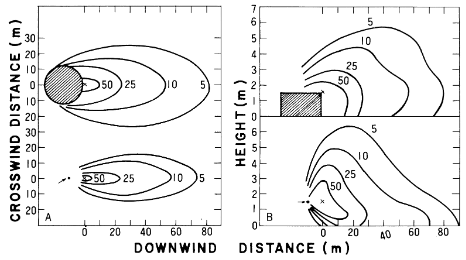
\includegraphics[]{diffusion-example-Okubo2001.png}
    \caption{The diffusion model describe the spread, motion, and evolution of a chemical, population or physical property over time. \cite{Okubo2001}.}
    \label{fig:diffusion-model-teaser}    
\end{figure}

Reaction-diffusion models are fundamental tools in mathematical biology and ecology, providing insights into the complex patterns observed in natural ecosystems. These models combine chemical or biological reactions (reaction) with movement through space (diffusion) to describe processes such as population dynamics, infectious disease spread, and ecological invasions \cite{Cosner2008}.

Initially developed to explain phenomena in chemistry and physics, reaction-diffusion models have been adapted to ecological contexts to simulate scenarios where organisms interact with each other and their environment over space and time. The application of these models in ecology helps in understanding how patterns of distribution and abundance arise, how they persist, and how they might change under various environmental pressures.

The concept of reaction-diffusion was initially introduced in the early 20th century by mathematician Alan Turing explored how non-uniform patterns emerge through mechanisms of chemical reaction and diffusion in \citep{Turing1952}. Turing's theories laid the groundwork for understanding pattern formation in biological systems, including those seen in animal coats and developmental processes.

The adaptation of reaction-diffusion models to ecological contexts began several decades later as ecologists camne to explain spatial phenomena such as the spread of invasive species, the maintenance of species diversity, and the formation of vegetation patterns. These models provided a mathematical framework to simulate and predict the dynamics of complex biological systems influenced by both local interactions and spatial movement.

Reaction-diffusion models describe the spatial and temporal evolution of populations, chemicals, or other ecological entities that interact (reaction) and spread (diffusion) through a medium. These models are widely used in ecosystem simulations to understand population dynamics, species dispersal, disease spread, and spatial pattern formation in ecological systems.

In the context of ecology, a reaction-diffusion model typically represents:
\begin{Itemize}
    \Item{} Reaction: Local changes in population density due to birth, death, predation, or competition.
    \Item{} Diffusion: Movement of individuals or species across space due to random dispersal or environmental factors.
\end{Itemize}
These models help ecologists predict how populations evolve over time and across space, providing insights into species survival, biodiversity, and ecosystem stability.

The classical reaction-diffusion equation is expressed as:

\begin{align}
    \label{eq:env-obj-classic-reaction-diffusion}
    \frac{\partial u (x, t)}{\partial t} = D \nabla^2 u(x, t) + R(u)
\end{align}

where $u(x,t)$ represents the population density (or concentration of a substance) at position $x$ and at time $t$, $D$ is the diffusion coefficient, determining the rate of spatial spread. $\nabla^2 u$ is the Laplacian operator, representing diffusion across space and $R(u)$ is the reaction term, which models growth, decay, or interactions between species.

\subsubsection{Diffusion term}
Diffusion is a fundamental process in ecological modeling that describes how individuals or substances spread across space due to random movement or environmental influences. In ecosystems, diffusion can model species dispersal, nutrient transport, disease spread, and invasive species expansion.

In mathematical models, diffusion is typically represented as a term in partial differential equations that governs how population densities change over time and space. While many ecological models assume isotropic diffusion (movement occurs equally in all directions), anisotropic diffusion provides a more realistic representation of species movement in structured or heterogeneous landscapes.

However, when diffusion is anisotropic, the diffusion coefficient varies depending on direction, and we must generalize the equation (\cref{eq:env-obj-classic-reaction-diffusion}) by introducing a diffusion tensor $\tensor{D}$ \cite{Ramos2024}:
\begin{align}
    \label{eq:env-obj-reaction-diffusion}
    \frac{\partial u (x, t)}{\partial t} = \nabla \cdot (\tensor{D} \nabla u(x, t)) + R(u)
\end{align}

The tensor $\tensor{D}$ can now encompass the effect of relief and environmental factors like wind and currents in the spread of a species. When diffusion is isotropic, $\tensor{D} = D\tensor{I}$, reducing the equation to the classic isotropic form.

Anisotropic diffusion is particularly useful in ecological modeling where movement rates are not uniform due to environmental structures or organism behavior. For example, wind influences the spread of pollen, seeds, and insect populations, leading to anisotropic diffusion. Similarly, marine organisms or pollutants diffuse anisotropically in ocean currents.
Invasive species may spread preferentially along corridors such as rivers or roads, causing asymmetric diffusion. In ecosystems where microorganisms move in response to chemical gradients (chemotaxis), anisotropic diffusion better models movement patterns.

We may generalize the reaction-diffusion equation to account for both internal (density, species interaction, ...) and external (environmental factor, relief, seasonality, ...) influences on diffusion by slightly rewriting \cref{eq:env-obj-reaction-diffusion}:
\begin{align}
    \frac{\partial u}{\partial t} = \nabla \cdot (\tensor{D(*)} \nabla u) + R(u)
\end{align}
where $\tensor{D(*)}$  is a diffusion tensor dynamically defined by any relevant internal or external property of the system. For example:
\begin{Itemize}
    \Item{} A density-dependent diffusion can be expressed as $\tensor{D(*)} = \tensor{D} u^m$, allowing for crowding or dispersal-limited movement \cite{Zhu2023}.
    \Item{} A seasonal dispersal effect can be incorporated as $\tensor{D(*)} = \tensor{D} (1 + A cos(\omega t) )$, where dispersal varies cyclically over time \cite{Katriel2021}.
    \Item{} A spatially varying diffusion may be defined as $\tensor{D(*)} = \tensor{D} f(x)$, such as the patchy diffusion formulation used in metapopulation models \cite{Czaran1998}:
    \begin{align}
        \tensor{D(*)} = \tensor{D} \begin{dcases}
            D_1&, x \in \text{habitable patch} \\
            D_2&, x \in \text{hostile patch}
        \end{dcases}
    \end{align}
    \Item{} An anomalous diffusion like the inclusion of Lévy flight term, incorporating random long distance jumps can be expressed as $\tensor{D(*)} = \tensor{D} u^m + \noise L(t)$ \cite{Humphries2014,Chechkin2008}.
\end{Itemize}

This generalized form enables the integration of anisotropic effects, landscape heterogeneity, and adaptive movement behaviors within reaction-diffusion models, making it highly applicable to ecological and biological systems.

\subsubsection{Reaction term}
In physics and chemistry, the reaction $R(u)$ term describes how substances are produced or consumed in a system. Some common reaction formulations include:

\begin{Itemize}
    \Item{} Linear reaction terms (exponential growth with $\lambda > 0$ or decay $\lambda < 0$) as in the radioactive decay formulation:
    $$ R(u) = \lambda u $$
    \Item{} Second-order reactions, usually found in chemical reactions between two molecules:
    $$ R(u, v) = \alpha u v$$
    \AltTextImage{
        \Item{} Turing pattern-forming systems proposed by Alan Turing to explain stripe and spot formations in animal coat patterns and chemical reactions \cite{Turing1952,Shoji2002}
        $$ R(u, v) = \begin{dcases}
            f(u, v) & \text{(Activator)} \\
            g(u, v) & \text{(Inhibitor)}
        \end{dcases}$$
    }{turing_patterns.png}{Turing patterns on animals}{fig:env-obj-turing-pattern}
\end{Itemize}

On the other hand, in ecology, the reaction term models population growth, competition, predation, and ecosystem interactions \cite{Brauer2012}. Some of the most important ecological reaction terms are:
\begin{Itemize}
    \Item{} The logistic growth, that describes a single species population growth in a limited-resource environment, is defined with a growth rate $r$ and a carrying capacity $K$ \cite{Verhulst1844}:
    $$ R(u) = r u \left( 1 - \frac{u}{K} \right)$$
    \Item{} The Lotka-Volterra competition model, that describe the trophic interactions between two or more species, for which the reaction-diffusion equations take into account each other species:
    \begin{align}
        \frac{\partial u_i}{\partial t} = r_i u_i \left( 1 - \frac{\sum_{j=1}^N a_{ij} u_j}{K_i} \right)
    \end{align}
    with $N$ representing the number of species and $a_{ij}$ the interaction coefficient (how strongly the species $u_j$ inhibit the species $u_i$). \\
    This formulation can also be rewritten in a vectorized form as the generalized Lotka-Volterra equation:
    \begin{align}
        \tensor{f} = \tensor{r} - \tensor{A} \tensor{u}
    \end{align}
    where $\tensor{f} = (f_1, f_2, ..., f_N)^\intercal$ represents the per capita growth rates of all species, $\tensor{r} = (r_1, r_2, ..., r_N)^\intercal$ is the intrinsic growth rate vector, $\tensor{u} = (u_1, u_2, ..., u_N)^\intercal$ is the species population vector and $\tensor{A}$ is the interaction matrix, with elements $a_{ij}$ describing the effect of species $j$ on species $i$.
    
    Since population growth depends on the per capita growth rate, the full population dynamics equation follows:
    \begin{align}
        \frac{\partial \tensor{u}}{\partial t} = \tensor{u} \circ \tensor{f}
    \end{align}
    where $\circ$ represents the element-wise product, ensuring that each species' growth depends on both its population size and its per capita growth rate.
\end{Itemize}


\subsubsection{Advection}
In vegetation ecosystem modeling, advection refers to the directed transport of biological or environmental variables under the influence of external forces such as wind, water flow, or slope. Unlike diffusion, which describes random movement, advection introduces a preferred direction of transport, significantly influencing ecosystem dynamics \cite{Burger2020}. 

Mathematically, the advection-diffusion-reaction equation (or "scalar transport equations" \cite{Baukal2000}) extends the classical reaction-diffusion model by adding a velocity field $\field{v}$ that governs directed movement:
\begin{align}
    \frac{\partial u}{\partial t} + \field{v} \cdot \nabla u = \nabla \cdot \left( \tensor{D} \nabla u \right) + R(u)
\end{align}

In physics, the transport of a property like heat is coupled by the diffusion process, and the advection term $\field{v} \cdot \nabla u$ may be incorporated in the diffusion coefficient $\tensor{D}$ to form the "convection term". In this work we will seperate the advection term and the diffusion term for clarity.

Wind is a major dispersal mechanism for many plant species, affecting seed distribution, plant competition, and biodiversity. The dispersal efficiency of seeds and pollen depends on wind velocity, turbulence, and interactions with terrain features. In flat landscapes, wind disperses seeds relatively uniformly; however, in complex terrains, wind speed and direction are influenced by topography, vegetation cover, and atmospheric conditions. Wind channeled through valleys may enhance seed deposition in lowland areas, while mountain ridges and abrupt elevation changes can create wind shadows, reducing dispersal effectiveness.

The dispersal of seeds can be modeled using a advection-diffusion equation:
\begin{align}
    \frac{\partial S}{\partial t} + \field{v} \cdot \nabla S = \nabla \cdot (\tensor{D}_s \nabla S) - \lambda S
\end{align}
with $S(x, t)$ the seed density at position $x$ and time $t$ and $\lambda$ a mortality rate due to environment constraints or predation.

A stochastic modelling of turbulent regime could be added to the velocity field with a stochastic noise term:
\begin{align}
    \frac{\partial S}{\partial t} + (\field{v} + \sigma(x, t)) \cdot \nabla S = \nabla \cdot (\tensor{D}_s \nabla S) - \lambda S
\end{align}


On another hand, soil moisture distribution is essential for vegetation survival and ecosystem stability. The movement of water through soil is governed by surface runoff, subsurface infiltration, and capillary action, which are affected by slope, soil texture, and plant uptake rates. In hilly or mountainous regions, gravity-driven water flow dominates soil moisture distribution, creating hydrological gradients that shape vegetation structure.

The movement of soil moisture can be approximated by the Soil Moisture Velocity Equation \cite{Ogden2017}, a modified form of the Richards equation:
\begin{align}
    \frac{\partial W}{\partial t} + \field{v} \cdot \nabla W = \nabla \cdot (D_W \nabla W ) - S
\end{align}
with $W(x, t)$ the water concentration at position $x$ and time $t$, $D_W$ the water diffusion coefficient, $S$ the plant water uptake (the amount of water absorbed or transpired, mainly by the roots of vegetation \cite{Peters2020,Shanin2015}), and $\field{v} = - K g \hat z$ a simplified velocity field provided by the slope hindered by the hydraulic conductivity $K$.

Steeper slopes enhance runoff, reducing soil water retention and increasing drought susceptibility in these regions. Conversely, water accumulates in lowland areas, promoting denser vegetation and the formation of wetlands or riparian ecosystems. As a result, topography directly influences plant distribution, with drought-resistant species dominating slopes and water-demanding species thriving in valleys.

We find in the advection-reaction-diffusion equation a general way to represent a multitude of natural phenomena: from the propagation of bacteria, prey and predators, to the spread of nutrients, of water, or even of fire \cite{Hadrich2021}. 






% The domain of ecosystem simulation is mainly focused on the simulation of plant growth, so this state of the art will be mostly based on it. 

% In an ecosystem, every element within the system has an impact on its surroundings, and accurately simulating physical properties like shading, heat, and humidity can require immense computational power. To address this, instead of simulating these properties individually for each object, they can be represented as scalar fields that span the entire scene. These scalar fields, which may represent temperature, humidity, or occlusion, are locally influenced by nearby objects and terrain features, such as trees casting shadows or buildings radiating heat. This approach, as described in \cite{Grosbellet2016, Guerin2016a}, allows for the environment's physical properties to be computed in a more efficient manner. By simplifying the complex interactions into these localized scalar fields, they called environmental objects, their method provides a scalable system that can handle large and detailed scenes. This system effectively renders scene details, such as snow accumulation or leaf distribution, in a way that is visually plausible, ensuring realistic results without the need for exhaustive simulations. 
% %In a similar way, other works represent the wind flow as a composition of local vector fields \cite{Wejchert1991}, avoiding complex fluid simulation while providing user control in a lightweight model. We extend these works by incorporating a time-evolution system such that the scene can be dynamic.
% In a similar approach, parallely Wejchert and Haumann \cite{Wejchert1991} and Sims \cite{Sims1990} represent wind flow as a composition of local vector fields, known as "flow primitives", which can be combined to simulate complex fluid behavior. This method simplifies the computation by avoiding full fluid simulations, instead offering a lightweight model that allows for intuitive user control over the flow dynamics.
% By combining these approaches, we can create dynamic ecosystems where environmental effects and fluid flows interact in a plausible manner, while requiring a low computation effort and preserving a high user control.

% % \subsubsection{Vegetation modeling}
% % \citep{Lane2002} Uses L-System to create a forest that then starts a self-thining process, which mean that larger and more mature vegetation will eliminate weaker species around them, simulating shadowing. The propagation of a given species is given using a kernel, controlling whever two individuals should prefer being close to each other or far away instead. This kernel is provided for each pair of species, simulating cohabitation and competition. The simulation parameters are fine-tuned by hand to resemble to biologically coherent scenes. \\ 




% \subsubsection{Distance-based instantiation}
% Most methods for ecosystem modeling consider the distance between each entity to spawn a new entity, without considering other environmental factors. This method is efficient and creates realistic results in a small scale scene, where the environment properties are almost identical in the whole terrain. Silviology, the study of forests, is often encompassed by this methodology as there are few variations inside the habitat due to the protection of the forest itself against wind, humidity and storms. 

% The grid-based approach of forest generation, 
% These models often used a grid-based approach, dividing space into discrete cells that represented the smallest spatial unit of interest. Each cell could house a plant or community and interact with its neighbors. This era saw the use of cellular automata and other grid-based systems which allowed for the simulation of spatial processes and interactions at various scales.

% % \citep{Benes2003} Simulate an ecosystem as multiple agents with different behaviours take care of plants to simulate cultivated areas \\ 

% In grid-based models, space is divided into discrete cells. Each cell is treated as a homogeneous unit within which certain properties are assumed to be uniform. The model defines how these cells interact with each other based on their proximity and shared boundaries. Each cell can hold different data values representing these attributes, allowing the model to simulate how spatial heterogeneity influences ecological dynamics. This type of model share a high similarity with cellular automata to simulate local interactions as each cell usually influence its direct neighbor cells. Through this method, the simulation of disturbances that spreads (like fire or disease) \cite{Wojtek2022}.

% On the other hand, the individual-based modeling (IBM) principle is that the system's behavior emerges from the actions and interactions of its individual components rather than from overarching equations that govern system-level changes. Each individual (or "agent") in an IBM can represent an organism, such as a plant or an animal, and is modeled with unique traits and decision-making rules that determine its behavior. Since each agent can be uniquely defined, IBMs are particularly suited to exploring how heterogeneity among individuals affects the dynamics of the entire system. The agents in this model may evolve in a discrete or continuous space. This method has been used for representing mobile agents (like gardeners in \cite{Benes2003}), but also plants \cite{Deussen1998}, in which each individual is spawn randomly in a landscape and with a Zone of Influence (ZOI) described by a disk of radius randomly affected depending on its species. When two individuals' ZOI are intersecting, one of the individuals is removed.

% Effectively, a tree growing too close to another one may not be able to survive due to lack of light or ressources from the ground. In the Field of Neihborhood method (FON) \cite{Berger2000}, the introduction of fields fills a gap between IBM methods that looks at each individual and grid-based methods that affect the space around each individual. The radius-based instanciation incrementally add new entities in the scene by introducing a radius around each tree dependant on its height. \cite{Alsweis2005} simulates the growth of each tree, with multiple species which have different effect radius. At each simulation step, a new tree is spawn, allowing for a continuous evolution of the ecosystem in a competition for space and light. 

% \citep{Alsweis2006} Optimisation of the previous method with (aperiodic) Wang Tiles \\ 

% \citep{Weier2013} Speeds the rendering time by precomputing a Poisson Disk Distribution in Wang tiles. This method allows for an aperiodic distribution without the need to compute on the fly the position of individual trees. \\

% \citep{DoNascimento2018} Propose an adaptation of distance-based instantiation (initially proposed by \citep{Hammes2001}) for the GPU by classifying the vegetation in 3 classes depending on their height (L1, L2, L3). A first instantiation is done for the larger vegetation (L1) on a $N \times N$ buffer, which influence the position of the L2 elements on a $2N \times 2N$ to simulate shading, and identically the instantiation on a $4N \times 4N$ buffer for L3 elements. \\ 

% \citep{Emilien2015a} Focuses their work on point distribution reproduction from examples. \\ 

% \citep{Makowski2019}  \\ 
% \citep{Seidl2012}  \\ 
% \citep{Seidl2011}  \\ 
% ...

% \subsubsection{Addition of abiotic factors}

% \citep{Gain2017} Improves the previous method by combining point distribution with terrain analysis to extract rules, meeting a balance between user control and realism. \\ 

% \citep{Kapp2020}  Learn the density of L1, L2 and L3 layers through deep learning, in order to avoid the use of classic statistical models that cannot capture the fine-scale complexities. Then the distribution of each species is done using the classic point distribution following an adaptability function taking into account abiotic factors. \\ 

% \citep{Chng2011a} and \citep{Chng2011b} Very close to our system, using rules between agents to grow/evolve. But only available for point-objects \\ 

% \citep{Cordonnier2017b} Consider the environment to have moisture, luminosity and temperature, then describe in each cell a density of population (Eulerian method) instead of individuals. \\ 

% \citep{Peytavie2024a} Continues previous methods, using abiotic factors from the map, and add the effect of the deposition of dead woods (snags, logs,humus, ...) to modify the abiotic factors. From this, the inclusion of events like fires and diseases have an indirect impact on the ecosystem. \\ 

% The inclusion of fauna in the process is very rare \cite{Ecormier-Nocca2021}.

% \midConclusion



\section{Description of the method}
\label{sec:env-obj-pipeline}

In this section, we present the pipeline and processes that underpin our method. Our approach introduces the concept of \glosses{EnvObj}, simplified terrain features that interact with their surroundings to simulate complex ecosystem dynamics. These \glosses{EnvObj}, which can represent natural features such as trees, rivers, or rocks, influence and are influenced by scalar fields like temperature, humidity, and elevation. The method is structured into several key phases: initialization, where the foundational elements of the terrain and \glosses{EnvObj} are set up; an iterative generation process, where these \glosses{EnvObj} are instantiated and interact with their environment; and finally, the production of a sparse representation of the scene's features. This section details each of these phases, explaining how the system dynamically adapts to user input and environmental changes.

\subsection{Pipeline}

\begin{figure}[H]
    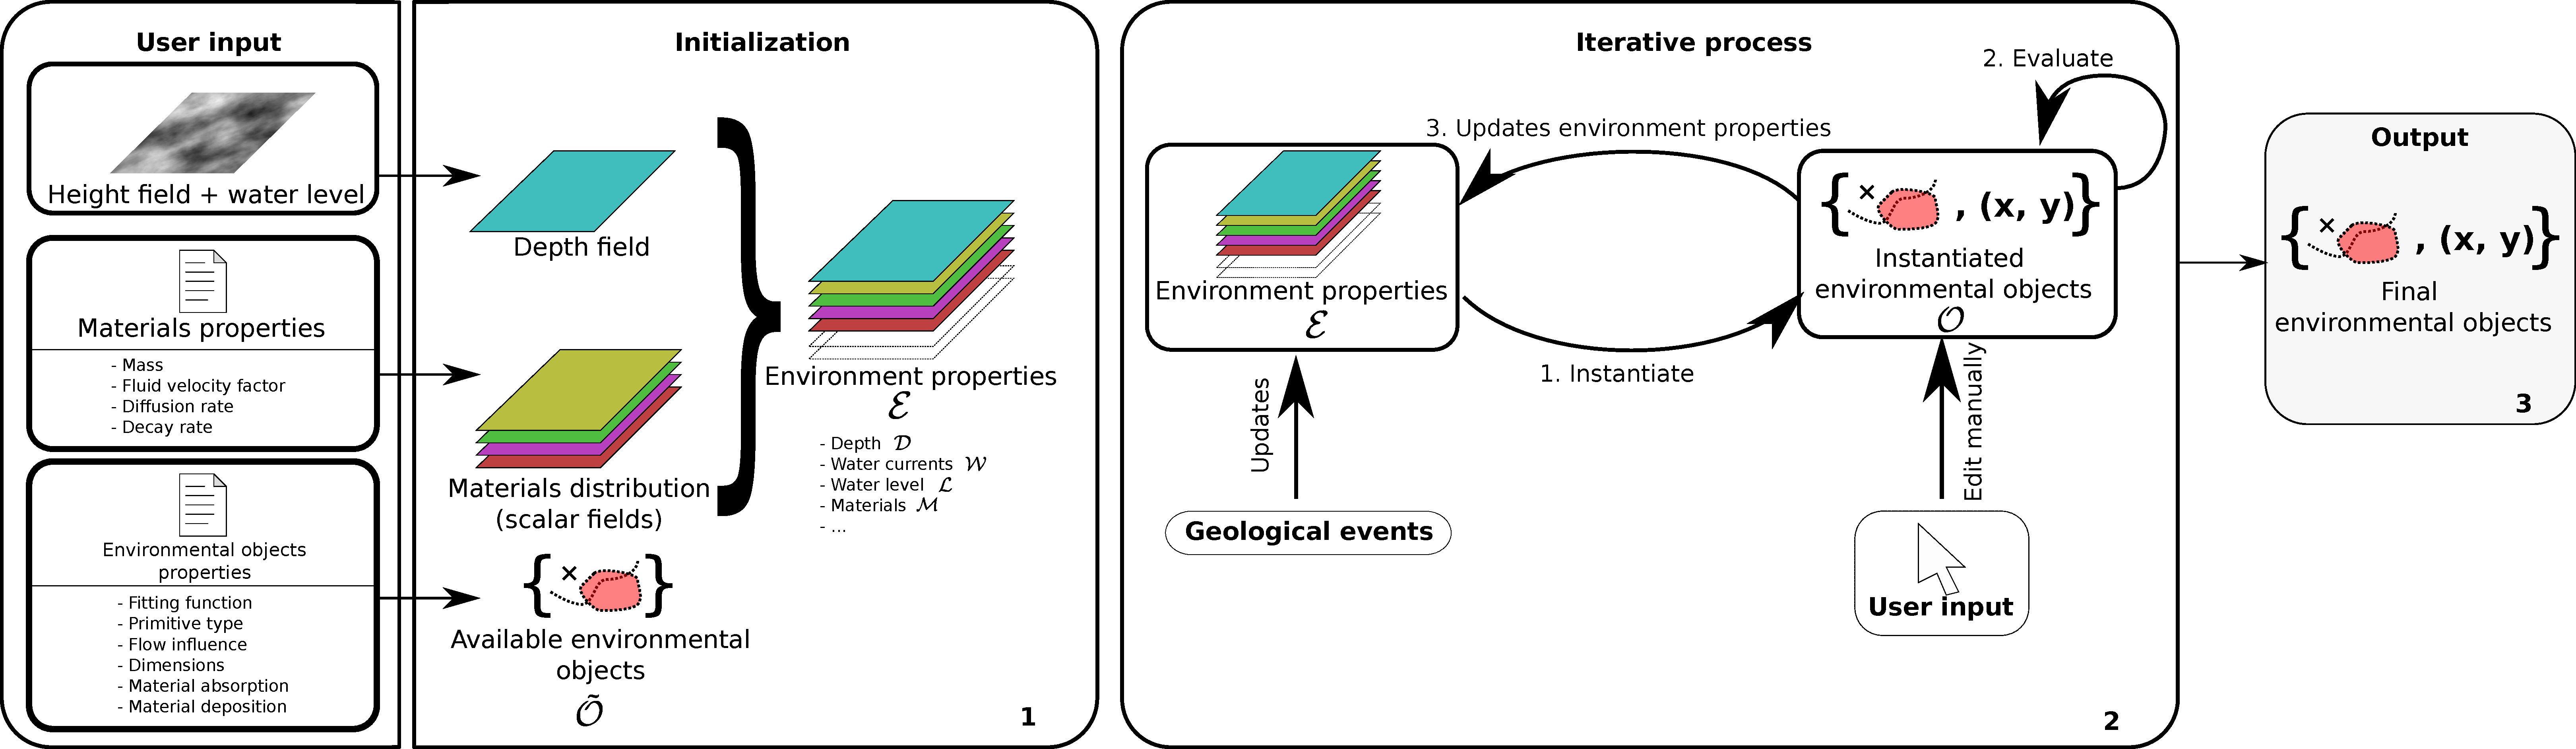
\includegraphics{pipeline.pdf}
    \caption{Overview of the pipeline of the method. The user provides as input an initial height field and sets the water level, as well as a definition of the \glosses{EnvMat} properties and \glosses{EnvObj} properties that will be used in the iterative process. These inputs are initialized as an initial set of \glosses{EnvObj} and scalar fields that represents the \glosses{EnvVal}. In the iterative loop, new \glosses{EnvObj} are instantiated using the current state of the environment at their optimal position. The existing \glosses{EnvObj} in the terrain reevaluate their \gloss{FitnessFunc} to grow or die and update the \glosses{EnvVal} locally. At each iteration, \glosses{GeoEvent} can update the \glosses{EnvVal}, while the user can interact directly with the \glosses{EnvObj}. The result of the whole process is a set of \glosses{EnvObj} which is a sparse representation of the features of the scene. }
    \label{fig:env-obj-pipeline}
\end{figure}

\subsubsection{Initialization}

The generation of the terrain is initialized using an initial height field $h$ and an initial water level $\Wlevel$. 
During this chapter we will include many features depending on altitude or depth, so we will use the shorthand notations $\height = h - \Wlevel$ and $\depth = -\height$. The height field provides variation on the altitude, which can influence the generation process of the scene.

The list of available \glosses{EnvObj} $\availableObjects$, representing the different features that can be present in the scene, are provided with their properties: type, size, \glosses{GenRule} and effects on the \glosses{EnvVal} (\cref{sec:env-obj-environmental-objects}). A target list of \glosses{EnvObj} $\targetObjects$ can be defined to control the final result of the generation.

Finally, different \glosses{EnvMat} are defined with their properties such as diffusion speed, mass, decay rate and influence from the water currents. An initial environment configuration resulting from the initial height field $\height$ and water level $\Wlevel$, the \glosses{EnvMat} distribution $\material$ (represented as scalar fields $\material: \R^2 \to \R$) and water currents $\Water$ (as a vector field $\Water: \R^2 \to \R^2$) will be used by the \glosses{EnvObj} of the scene to simulate their growth and spawn at the most probable position. The \glosses{EnvVal} are noted $\environment = (\depth, \Water, \Wlevel, \material)$ (\cref{sec:env-obj-communication}).

The definition of \glosses{EnvObj}' properties and \glosses{EnvVal} is done with field experts, providing the pertinent parameters required to model the evolution of the terrain features using expert knowledge (\cref{sec:state-of-the-art_biology}). 

The generation phase starts with an initial set of \glosses{EnvObj} present in the scene, which can optionally be pre-filled.

\subsubsection{Generation process} 

%- Main loop
Once the initialization phase is done, the generation begins. The generation process is incremental and its main loop is composed of two different steps: the instantiation of new \glosses{EnvObj} then the update of the environment. This loop is repeated until the user is satisfied with the look of his environment or following rules like a number of features threshold or a targeted list of \glosses{EnvObj} as described in the layout planner defined in \citep{Tutenel2009}.


\subsubsubsection{Instantiation}
% - Object instantiation
At each iteration, new \glosses{EnvObj} can be created at their most fitting locations if possible. The \glosses{GenRule} provided in the initialization phase are used to find an optimal position from stochastic sampling (\cref{sec:env-obj-generation-rules}). 
All \glosses{EnvObj} are evaluating their state analytically using a \gloss{FitnessFunc} and a \gloss{FittingFunc} provided as input (\cref{sec:env-obj-generation-rules}).

\subsubsubsection{Environment update}
% Once the new objects are instantiated, the process can continue.
% - Environment update
Once the instantiation step is done, the \glosses{EnvVal} are updated by each \gloss{EnvObj} through \glosses{EnvModif}, which depose and absorb some of the \glosses{EnvMat} $\material$ (\cref{sec:env-obj-materials}) while modifying the water currents $\Water$ (\cref{sec:env-obj-water-currents}) and the height field $\height$ around them. Finally, water currents and terrain slope displace \glosses{EnvMat} of the terrain until reaching a dynamic equilibrium in the environment at each iteration.

% We consider the water currents to be a steady-state flow, allowing us to remove the variation from time in the flow equations.
% The water currents are updated locally by each \gloss{EnvObj} using an analytical form $W^*(\p) = W(\p) + \omega(\p)$.
During the generation process, the user can alter directly the distribution and shapes of the \glosses{EnvObj} (\cref{sec:env-obj-manual-interaction}) and perturb the generation process by planning \glosses{GeoEvent} that have impacts on the \glosses{EnvVal} (\cref{sec:env-obj-events}).


\subsubsection{Output}
% - Output result
The output of our system is a set of \glosses{EnvObj} disposed in the plane. We do not provide the 3D representation of the \glosses{EnvObj} in this chapter, letting the user define the rendering method. The figures used in the chapter use a mix of implicit surfaces and triangular meshes.

\subsection{\Glosses{EnvObj} }
\label{sec:env-obj-environmental-objects}

\begin{figure}
    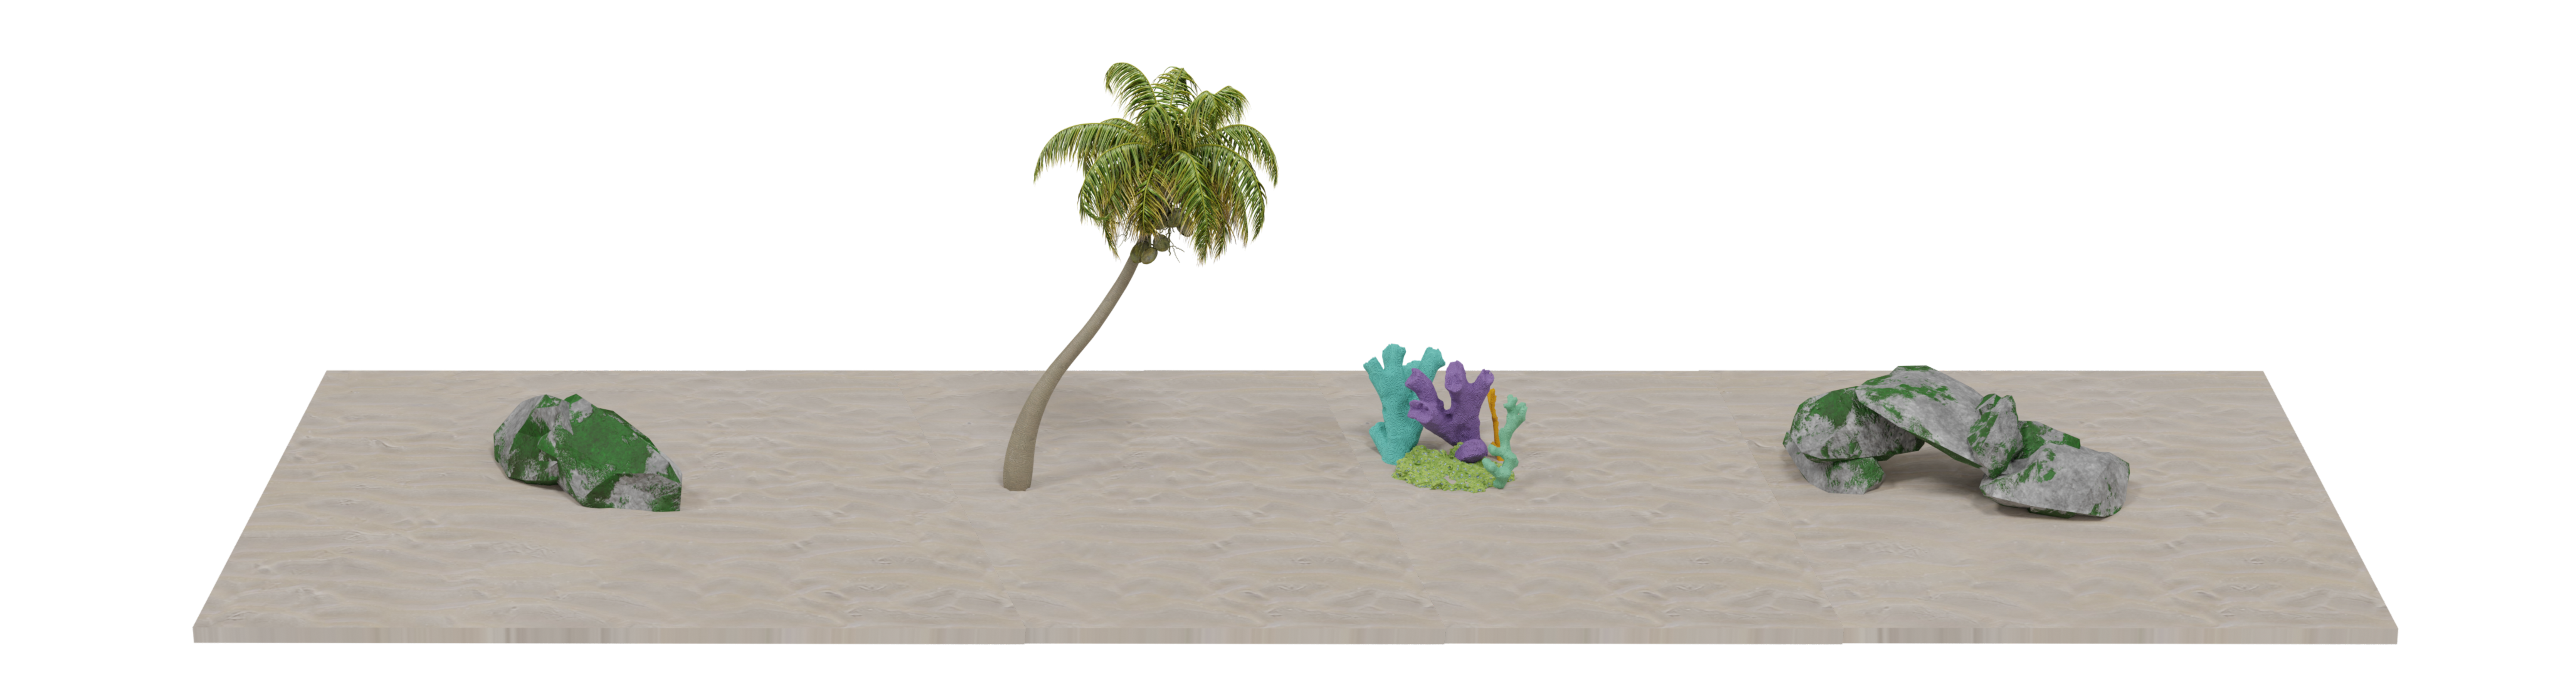
\includegraphics{assets-demo.pdf}
    \caption{\Glosses{EnvObj} can be visualized by 3D triangular meshes. From left to right: rocks, trees, corals, arches.}
    \label{fig:env-obj-assets}
\end{figure}
A geographical feature, also called object or entity, is defined as a discrete phenomenon located at or near the Earth's surface, relevant in geography and geographic information science (GIScience). It represents geographic information that can be depicted in maps, geographic information systems (GIS), and other forms of geographic media. This term includes both natural and human-made objects, ranging from tangible items like buildings or trees to intangible concepts like neighborhoods or savana. Features are distinct entities with defined boundaries, differentiating them from continuous geographic masses or processes occurring over time. They can be categorized as natural features, such as ecosystems, biomes, water bodies, and landforms, or artificial features, such as settlements, administrative regions, and engineered constructs. Geographic features are described by characteristics including identity, existence, classification, relationships with other features, location, attributes, and temporal aspects. Information about these features is stored in geographic databases using models like GIS datasets, which organize and represent these features in structured formats. As the term "feature" is overused in computer science, we will use the term \gloss{EnvObj} in this work.

\AltTextImage{
Each \gloss{EnvObj} is shaped with a simple geometric shape called a "skeleton" that defines where it is located and how it fits into the environment. The \gloss{Skeleton} can either be, as used in cartography, a point, a curve or a region. We will then refer to our \glosses{EnvObj} as point-based, curve-based or region-based, respectively.  
These \glosses{EnvObj} interact with the environment $\environment$ by changing local conditions using the \glosses{EnvModif}. For example, the presence of a river might increase the moisture in the surrounding area, while a mountain might induce more rockiness in the soil composition. They can also absorb changes from the environment, such as a forest taking in humidity from the air.
The placement of \gloss{EnvObj} is determined by a \gloss{FitnessFunc} $\fitnessFunc$, which evaluates how suitable a location is based on the \glosses{EnvVal}. Once a suitable location is found, the \gloss{FittingFunc} optimizes the shape and position of the entity to fit as best as possible into the environment $\fittingFunc$.
}{Env-obj-scheme1.png}{Environmental objects, from 2D (left) to their 3D geometry (right)}{fig:env-objs_example-scheme1}

%This approach allows us to "spawn" new entities based on rough altitude estimates, ensuring that their placement is contextually appropriate while deferring the detailed computation of their final shape to a later stage, if required by the user.
% The coarse height function thus acts as a middle between the semantic modeling of terrain and the precise 3D modeling. It provides enough information to make informed decisions about \glosses{EnvObj} placement and \glosses{EnvMat} while preserving the flexibility to integrate more detailed modeling techniques. This method ensures that the terrain generation remains interactive and scalable, allowing for the dynamic and realistic placement of entities in complex landscapes without being tied to the immediate computation of detailed topography.

% \Glosses{EnvObj} are rule-based objects following rules depending on their local environment for evaluation their state in their life cycle. We can see them as a life form in the way that they are created and eroded with time. During their lifetime, they influence their local environment by depositing and absorbing \glosses{EnvMat} around them and influencing the water currents. The environment objects are described spatially as a single point, a parametric curve or a region.


\subsection{\Glosses{EnvVal} }
\label{sec:env-obj-communication}

In geography, a "field" refers to a continuous spatial phenomenon across a region where each point has a specific value of a variable, unlike discrete objects with distinct boundaries. Fields can be scalar, representing a single value at every point (like temperature or elevation), or vector, representing quantities with magnitude and direction (like wind velocity). Examples include topographic fields for elevation, climatic fields for temperature or precipitation, and magnetic fields for magnetic forces. Because of the ambiguous nature of the term "field" with mathematics and computer science, we will define the geographic fields as \gloss{EnvVal}.

In an ecosystem simulation, each actor of the ecosystem has an impact on all other actors, which results in an exponentially growing computation effort as the number of elements of the terrain increase. We avoid this problem by considering the \glosses{EnvVal} as a proxy to allow any \gloss{EnvObj} to interact with any other one. Each of the \gloss{EnvObj} have a local impact on the \glosses{EnvVal} without knowledge of neighboring \glosses{EnvObj}. This modification of the \glosses{EnvVal} are presented as the effect of \glosses{EnvModif} defined for each \gloss{EnvObj}. % can be due to an absorption and deposition of some material $\material$ or an influence on the water currents.

In this work, we have integrated vector \glosses{EnvVal} (e.g., water currents $\Water$) and scalar \glosses{EnvVal} (e.g., altitude $\height$, water level $\Wlevel$, and various material properties $\material$) under the unified term "environment," denoted as $\environment = \left( \height, \Water, \Wlevel, \material \right)$. The \glosses{EnvMat} represent abstract quantities such as the availability of sand, salt, moisture, or rocks at each point. It is important to emphasize that these materials are not to be visualized as physical layers stacked on the terrain surface. Instead, they should be understood as conceptual resource distributions that influence the environment and the behavior of \glosses{EnvObj}, rather than as something directly observable in the scene.

\subsubsection{\Glosses{EnvModif} $\environmentModif$}
The environment determine if a \gloss{EnvObj} does belong at a certain position. When a \gloss{EnvObj} is placed, its surrounding \glosses{EnvVal} can be affected though \glosses{EnvModif} noted $\environmentModif = (\heightModif, \waterModif, \nothing, \materialModif)$ defining a change of height $\heightModif$, changes in the water currents $\waterModif$ and \gloss{EnvMat} alteration $\materialModif$. 

\Glosses{EnvObj} are subject to altitude conditions. However, to maintain a clear distinction between semantic modeling and 3D modeling, we do not compute the exact physical shape or detailed height field of each \gloss{EnvObj}. Instead, we define a \gloss{CoarseHeight}, a parametric representation derived from the \gloss{Skeleton} to provide a rough estimate of the changes in elevation around it. This simplified model of how the \gloss{EnvObj} influences the surrounding terrain's altitude allows us to cheaply evaluate the potential presence of new entities that have altitude-dependent conditions without the need to perform expensive computations to generate a detailed height field of the entire terrain. 

Altering the vector field of the water currents $\Water$ is done by the composition of the effect $\waterModif$ of each object at a position $\p$ as introduced in \citep{Wejchert1991}, while we use the formulation of Kelvinlets \cite{DeGoes2017} in the computation of effect of each \gloss{EnvObj}.

Each \gloss{EnvObj} has intrinsic \glosses{EnvMat} that can be seen as "spreading" and "absorbed" around its skeleton over time. A coral reef may produce coral polyps and at the same time reduce the water currents. It grows thanks to the deposition of limestone from coral colonies. In our model, the colonies affect the \glosses{EnvVal} through the deposition of \gloss{EnvMat} $\materialModif_\text{limestone}$, which in turn, is absorbed by the coral reef, without a direct exchange between the two \glosses{EnvObj}.

The alteration of a scalar \gloss{EnvVal} is done by adding or removing some amount around the \gloss{Skeleton} of the \gloss{EnvObj} and diffusing it in the space, influenced by the water currents. We consider the system to be \gloss{SteadyState}, garantied by the introduction of a decay rate $\decay > 0$ in the computation of the diffusion and advection.



\section{Placement of \glosses{EnvObj} in an environment}
\label{sec:env-obj-generation-rules}

At each iteration of our algorithm, we want our \glosses{EnvObj} to be at plausible positions. We do not guaranty a temporal continuity between iterations as in \citep{Ecormier-Nocca2021}, so the objective is to add new \gloss{EnvObj} in order to satisfy the users wishes, while conserving the plausibility of the scene. Rather than "forming" these \glosses{EnvObj}, our method "reveals" them, much like a paleontologist uncovers fossils during an excavation. A paleontologist does not dig randomly across the Earth to find fossils; instead, they analyze the geological context to identify the most likely locations. Similarly, our method observes the environment and estimates where certain elements are likely to exist. For example, in hydrology, if a river appears to originate from nowhere, it might suggest the presence of a karstic river system upstream. In urban planning, if many roads converge at a certain point, it is reasonable to expect that a city is located there. This approach ensures that Semantic Terrain Entities are revealed in positions that are contextually appropriate and coherent within the landscape.

We will follow the same intuition using a \gloss{FitnessFunc} for each of the \gloss{EnvObj} that may be spawn in the terrain. The \gloss{FitnessFunc} defined $\fitnessFunc: \environment \to \R$ provides a score indicating how well the \gloss{EnvObj} may fit in this position. Evaluating this function at multiple position results in an approximation of the fitness map of the entity. Once the most probable position is found, we can find the most plausible shape of the \gloss{EnvObj} using the \gloss{FittingFunc} $\fittingFunc$.

For this task, we place a new elements required at the most plausible position using the analysis of the \gloss{FitnessFunc} of each \gloss{EnvObj}. We know that each \gloss{EnvObj} will modify the environment surrounding, which may make previously instantiated \glosses{EnvObj} unfitted. Knowing this,the goal is to add the new element at the position that will change the least the stability of the system. 

Genetic algorithms or Depth First Search algorithms could be used to try many possibilities until a local or global minimum could be found, but this would require a large processing power. Naive genetic algorithms would place a \gloss{EnvObj} at a certain position at each iteration and evaluate the stability of the environment, repreating this operation while varying slightly the position of the \glosses{EnvObj} or the type of \gloss{EnvObj} instantiated at each iteration, resulting in way too much computation to stay interactive. The Depth First Seach algorithms would require to compute all the possible combinations of \glosses{EnvObj} and positions which, given the fact that we want a continuous position in order to work multi-scale, would require to compute an incredibly high amount of possible configurations in order to find a plausible situation, on average. We will work with an evolutionary algorithm to find a compromise between fast computation and a satisfying result.

Our placing algorithm is done in two steps: first, it identifies the global location where a \gloss{EnvObj} best fits within the environment $\environment$ using its \gloss{FitnessFunc} $\fitnessFunc$, which evaluates the suitability of each point $\p$ based on the \glosses{EnvVal} $\environment_p$, including factors such as altitude $\height(\p)$, water current velocity and direction $\Water(\p)$, water level $\Wlevel(\p)$, and the availability of \gloss{EnvMat} $\material(\p)$. Second, once the most suitable location is identified, the algorithm determines the most plausible shape of the \gloss{EnvObj} using the \gloss{FittingFunc} $\fittingFunc$.

To ease the reading the functions $\fitnessFunc(\environment(\p))$ and $\fittingFunc(\environment(\p))$ with $\environment(\p)$ the \glosses{EnvVal} at the point $\p$ of the terrain are simplified to $\fitnessFunc(\p)$ and $\fittingFunc(\p)$ respectively.

% Our placing algorithm is done in two steps: first we estimate at which global location the \gloss{EnvObj} fits the most given an environment $\environment$ using its \gloss{FitnessFunc} $\fitnessFunc$, secondly we estimate the shape of the skeleton of this \gloss{EnvObj} should take given a \gloss{FittingFunc} $\fittingFunc$.

% \Glosses{GenRule} provides, for each \gloss{EnvObj}, a \gloss{FitnessFunc} $\fitnessFunc$ defining the most probable location for an \gloss{EnvObj} to be found. \Glosses{FitnessFunc}' parameters contains, for every point $\p$, the \glosses{EnvVal} $\environment_p$ (the altitude $\height(\p)$, the velocity and direction of the water currents $\Water(\p)$, the water level $\Wlevel(\p)$ and the amount of each \gloss{EnvMat} available $\material(\p)$).

\subsection{\Gloss{FitnessFunc} }

\begin{figure}
    \autofitgraphics[]{coral-erosion-example.pdf, rock-erosion-example.pdf}
    % 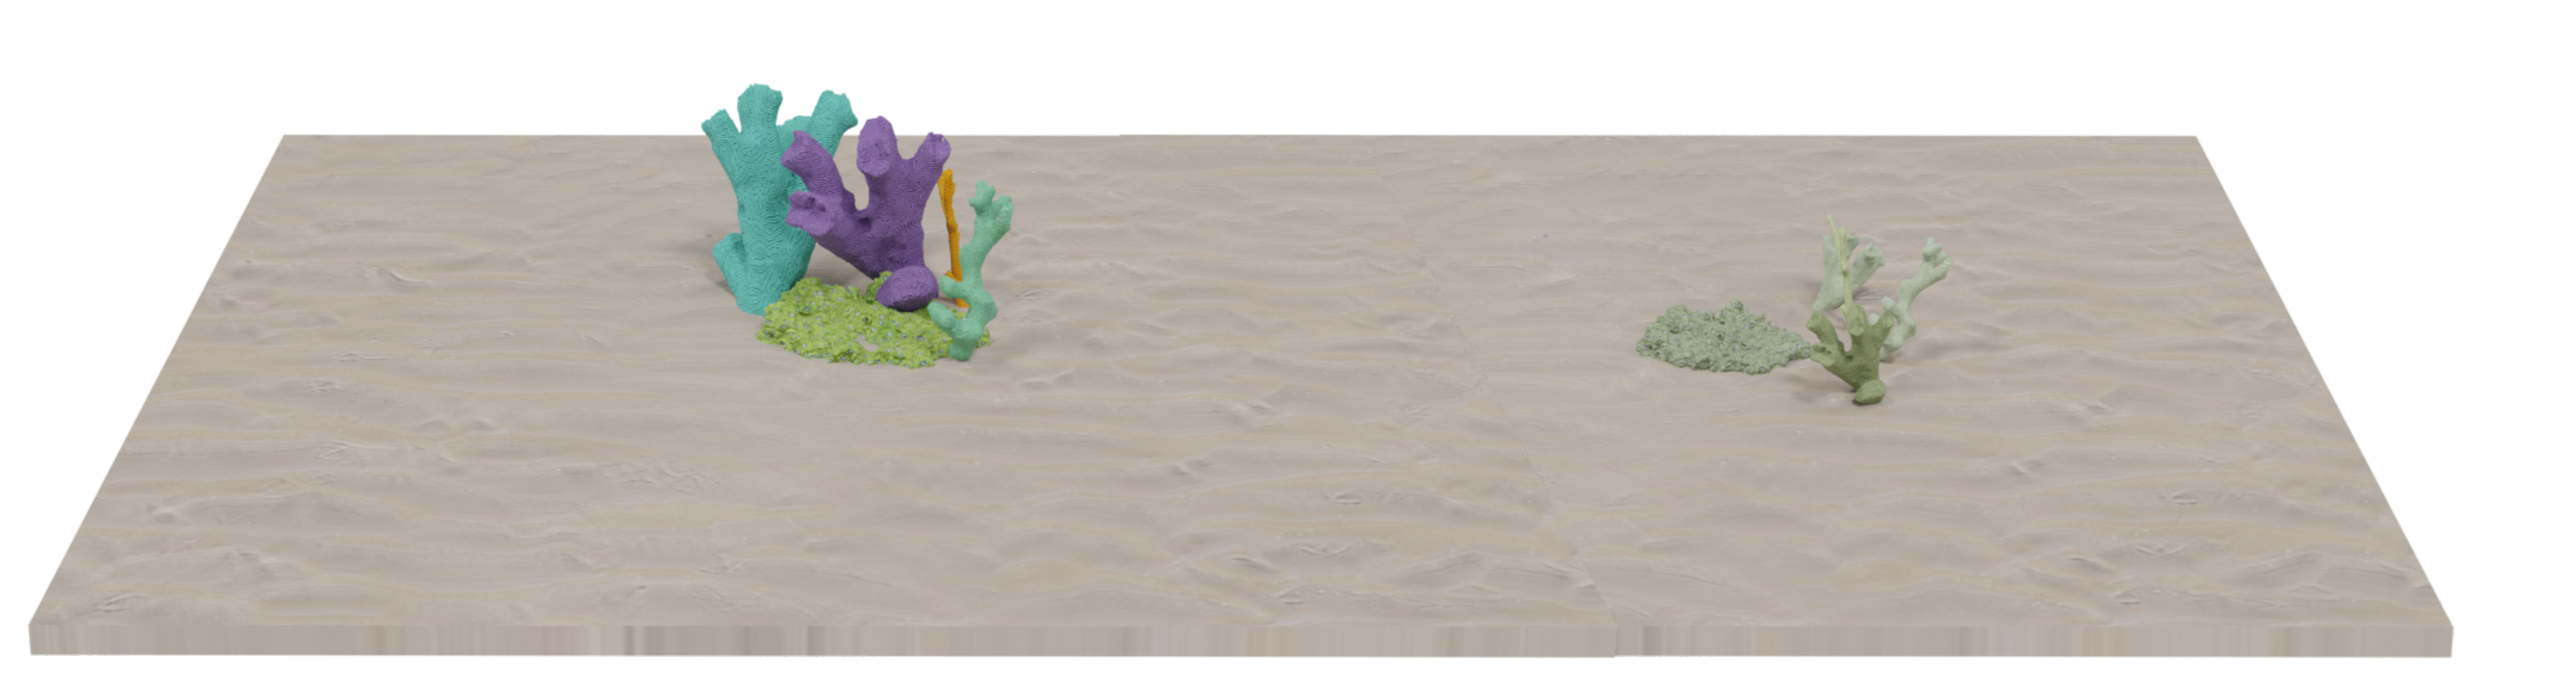
\includegraphics[width=.45\linewidth]{coral-erosion-example.pdf}
    % 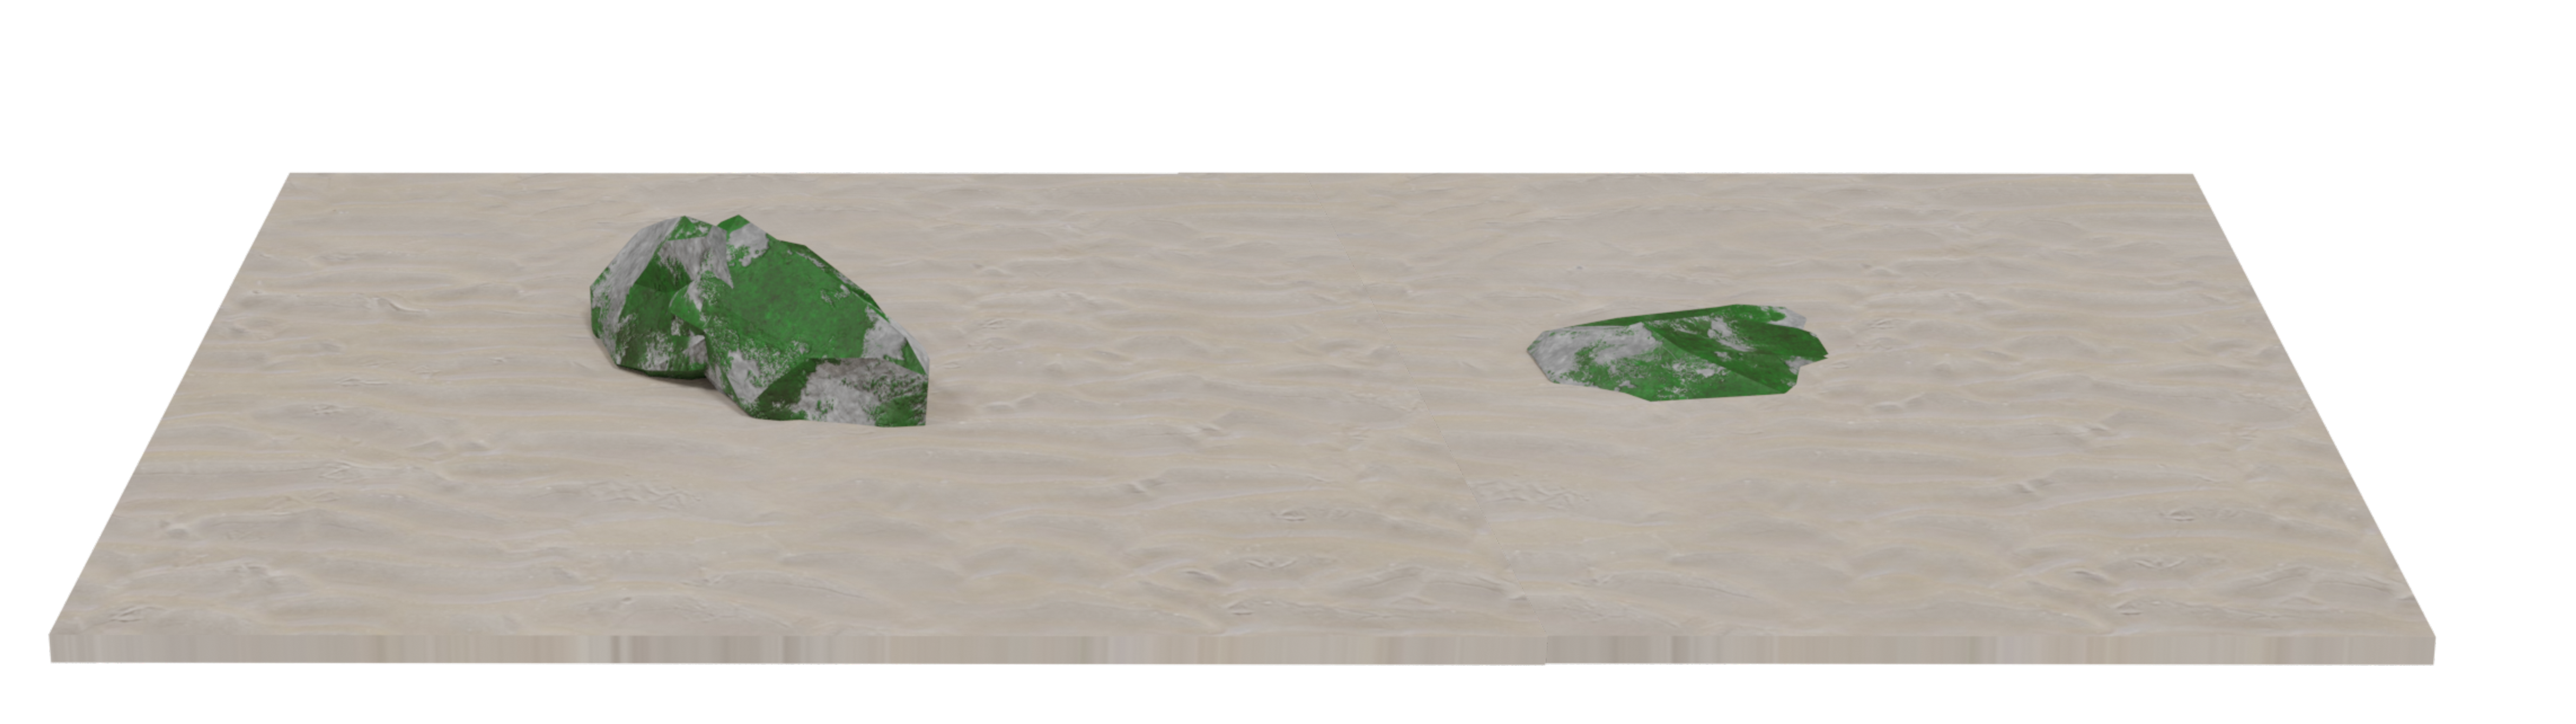
\includegraphics[width=.45\linewidth]{rock-erosion-example.pdf}
    \caption{While the \gloss{FitnessFunc} guides the position of the \glosses{EnvObj}, the \gloss{FittingFunc} provide an indication of the suitability of the \gloss{EnvObj} in its surroundings. This information is used to determine if the \gloss{EnvObj} should be removed, but may also be used for visual purposes to indicate unhealthy corals or eroded rocks. }
\end{figure}

"Darwinian fitness" refers to an organism's ability to survive and reproduce in its environment. It is a measure of how well-suited an organism is to its surroundings, and those with higher fitness are more likely to pass on their genes to the next generation. In a similar vein, the \gloss{FitnessFunc} of a \gloss{EnvObj} evaluates its suitability at a location in the terrain, extending the meaning to living features like forests and corals and non-living elements such as rivers, mountains, karsts, etc.

The fitness function is constructed by evaluating several environmental variables at a given location $\p$. These include altitude ($\height(\p)$) and its gradient ($\nabla \height(\p)$), the availability and gradient of various materials ($\material_i(\p)$ and $\nabla \material_i(\p)$), water current characteristics ($\Water(\p)$), and water level ($\Wlevel(\p)$). Altitude and its gradient can influence the placement of objects like rivers, which may prefer lower elevations, or forests, which might thrive on slopes. Each material, such as limestone, sand, or clay, is considered separately, and their availability and gradients at a location are crucial for determining the suitability of different \glosses{EnvObj}, such as a coral reef requiring specific substrates. The velocity and direction of water currents are essential for placing aquatic features or determining where erosion might occur, while the proximity to water influences the likelihood of placing wetlands, lakes, or other hydrological features.

% These environmental variables are typically combined in the fitness function, often expressed as a weighted sum, but not restricted to this form:

% \begin{align*}
%     \fitnessFunc(\p) = w_1 \cdot \height(\p) + w_2 \cdot \nabla \height(\p) + \sum_{i} \left( w_{3,i} \cdot \material_i(\p) + w_{4,i} \cdot \nabla \material_i(\p) \right) + w_5 \cdot \Water(\p) + w_6 \cdot \Wlevel(\p)
% \end{align*}

% Here, $w_1, w_2, w_{3,i}, w_{4,i}, w_5, w_6$ are weights that reflect the relative importance of each factor for the specific \gloss{EnvObj} being considered.

Different types of \glosses{EnvObj} require different criteria for their fitness evaluation. For example, a river might prioritize lower altitude and proximity to water currents, while a forest might prioritize higher altitude and specific material availability. The flexibility of the fitness function allows it to be customized for each \gloss{EnvObj}, ensuring that the generated terrain remains coherent and realistic.

\subsection{\Gloss{FittingFunc} }
The seed point of a spawning \gloss{EnvObj} is defined at the point $\p$ satisfying $\arg \max_\p \fitnessFunc(\p) $.
% a stochastic sampling of the plane. We propose different optimization means to find the optimal fitting position, depending on the \gloss{EnvObj} shape.

\subsubsection{Point-based \gloss{Skeleton}}
The spawning position of a punctual \gloss{EnvObj} is found at the local maxima of the \gloss{FittingFunc} from the seed point. While the \gloss{FittingFunc} doesn't have to be identical to the \gloss{FitnessFunc}, we usually use $\fittingFunc = \fitnessFunc$ for point-based \glosses{EnvObj}. If the two functions are different, the optimisation process simply follows the field's gradient $\nabla \fittingFunc$ until the local maxima is reached.

\subsubsection{Curve-based \gloss{Skeleton}}
% A curve can have different \glosses{GenRule}, making the definition of the functions easier depending if the \gloss{EnvObj}'s \gloss{Skeleton} has a notion of direction. It can either:
% \begin{Itemize}
%     \Item{} follow the gradient of the \gloss{FittingFunc} $\nabla \fittingFunc$, useful when the direction of the \gloss{Skeleton} has an importance like a river that has to run downhill,
%     % \Item{} follow the isocontour $\nabla \fittingFunc^\perp$, [WAIT, IS THAT NEEDED?]
%     \Item{} or optimize the energy of the function over its curve, like a coral reef that has to cover as much coral colonies as possible. % follow the heat points.
% \end{Itemize}

% \subsubsubsection{Following the gradient}
% Following the gradient of the \gloss{FittingFunc} $\nabla \fittingFunc$ is done by extending a curve from the seed point towards $\nabla \fittingFunc$ until reaching a local maximum while also following $-\nabla \fittingFunc$ until finding a local minimum. We stop the building process when our curve reaches a length limit $\Length$. 

% This \gloss{FittingFunc} strategy is efficient to describe rivers as we can set $\fittingFunc(\p) = \height(\p)$ to force it to always run downstream. 

% \subsubsubsection{Energy optimization}
The skeleton of a curve-based \gloss{EnvObj} is determined by the shape that fits the most given the environment it is added to. 
Using a modified version the Active Contours algorithm \cite{Kass1988}, we can minimize the energy $\energy$ for the parametric curve $\curve$ given $\energy(\curve) = \Einternal + \Eexternal + \Eshape + \Egradient$ with  
\begin{align}
    \label{eq:internal-energy-equation}
    \Einternal &= \Ainternal \left( \int_{\curve}{ \norm{\curve'(s)}^2 \, ds} + \int_{\curve}{ \norm{\curve''(s)}^2 \, ds}  \right) \\
    \Eexternal &= \Aexternal \int_{\curve}{ \fittingFunc(\curve(s)) \, ds } \\
    \Eshape    &= \Ashape \left( \Length - \int_{\curve}{ \, ds } \right)^2 \\
    \Egradient &= \Agradient \int_{C}{ \dot{C'(s)}{\Delta \fittingFunc(C(s))} \, ds }
\end{align}
In this configuration, $\Einternal$ induce a smooth continuity of the curve by reducing the spacing of each point while reducing the curvature. Another energy, $\Eexternal$ integrate the \gloss{FittingFunc} over the curve, often seen as an attractor of the points, that tries to descent the gradient to find local minima. At the same time, $\Eshape$ apply constraints on the curve shape, which, in this case, is to target a specific length $\Length$. As such, the curve search for an optimized shape given constraints in $\Eshape$ for minimizing $\Eexternal$. We introduced a new term $\Egradient$ in the energy computation that push the points of the curve in the direction of the slope of the \gloss{FittingFunc}, also providing an orientation for the curve.

If a steep coast can be found where the terrain slope is important near the water level, we can define $\fittingFunc = \abs{\height + 1} / \norm{\Delta \height}$, but no orientation is needed, thus we set $\Agradient = 0$. In this case, the curve will follow a path at the water level and spread its extremities over areas with a steep slope. A river may also be symbolized as a parametric curve, but we need to add information about the direction and magnitude of the slope.  As such, we can use $\fittingFunc = \height$ which forces the direction of the curve to fit with the terrain slope. The introduction of the gradient component provides also an orientation to shapes.

\AltTextImage{
    \subsubsubsection{Internal energy}
    The internal energy, already introduced in \citep{Kass1988} is composed of two components imposing penalities on the local properties of the points of the curve. The first derivative forces the points along the curve to be evenly spaced by minimizing the curve tension, while the second derivative restrict it from forming sharp corners. As our aim is to represent natural elements, we rarely find sharp elements and thus, keep the original definition from the Snake formulation.

    In \cref{fig:env-obj-snake-internal} we see the two different components of this energy minimisation: averaging the vector formed by the previous segment with the vector formed by the next segment, we can move the vertex to a position for which the two new segments equal in length. On the other hand, translating the vertex toward its projection minimizes the curvature at this vertex.
}{snake_algorithm_internal.png}{Internal energy minimization for one vertex is done by reducing the difference of length with the next and with the previous vertices, while reducing the curvature at this point. }{fig:env-obj-snake-internal}

\AltTextImage{
    \subsubsubsection{External energy}
    The external energy is also present in the original work. Using an external scalar field, each point of the curve is forced to follow the steepest slope of the field. The external field can be seen as an attractor for the curve.

    The energy is minimized when the vertex is positionned at the global maximum of the scalar field.
}{snake_algorithm_external.png}{The central vertex can optimize its external energy by translating in the same direction as the function gradient $\nabla \fitnessFunc$.}{fig:env-obj-snake-external}

\AltTextImage{
    \subsubsubsection{Shape energy}
    We introduced the shape energy, an energy defined on the whole curve to apply constraints on its final shape. As many natural features have a given dimension, we may add a constraint on the length of the \gloss{Skeleton}. 
}{snake_algorithm_shape.png}{The shape energy is minimized when the arc length of the curve $\curve$ is equal to a parameter $\Length$, obtainable by towards or in opposition of its neighbors. }{fig:env-obj-snake-shape}

\AltTextImage{
    \subsubsubsection{Gradient energy}
    In our application, having information about the orientation of \glosses{EnvObj} may be essential. For this purpose, we introduced a gradient energy component in the formulation. The equation impose that the direction of the curve at any point should be directed towards the gradient of the scalar field. As the external energy pushes points toward the lowest point of the scalar field, the gradient field restrict the gradient descent for the global curve into a specific way, which may feel more natural.
    
    During the optimization process, the gradient of the scalar field is already evaluated by the external energy optimization, so the addition of the gradient component is almost free.

}{snake_algorithm_gradient.png}{The gradient energy is minimize when the curve cross perpendicularly the gradient function. Black: the initial curve, Blue: a possible curve crossing the gradient. The scalar field is stylized to display isolines that the optimal curve has to cross.}{fig:env-obj-snake-gradient}


% \subsubsubsection{Position constraint}
% As the curve minimize its energy, it may fly far away from the initial seed point. We added a last constraint about the positioning of the curve such that the distance between t

% The internal energy $\Einternal$ force the shape continuity while the shape energy $\Eshape$ force the shape into a specific target length $\Length$, and finally $\Eimage$ that use the definition of the \gloss{FittingFunc} to attract the points of the curve toward a local minimum.

% While the first two possibilities are trivial, the later can also be optimized using the Active Contours algorithm by optimizing the energy $\energy = \Einternal + \Eshape$ with \eqref{eq:internal-energy-equation}. We applied a length constraint on the curves : 
% \begin{align*}
%     \Eshape = \left( \Length - \length \right)^2
% \end{align*}
% with $\length$ the curve's length and $\Length$ the target length. This algorithm is sensible to the initial shape of the curve, so we start with a straight line following the isolevel at the seed point.

\subsubsection{Region-based \gloss{Skeleton}}

Region-based \glosses{EnvObj} follows the same process than curve-based \glosses{EnvObj} to define their \gloss{Skeleton}, at the exception of the gradient energy $\Egradient$ which have null value on closed shapes. 

The resulting energy $\energy$ to minimize for a closed region whose borders are defined by the curve $\curve$ can then be expressed as $\energy(\curve) = \Einternal + \Eexternal + \Eshape$.

The internal energy is expressed identically as for curve-based \glosses{EnvObj}. The extenal energy however, has to be modified to take into account the interior of the region instead of only the borders. We will use the idea of the Chan-Vese algorithm, differentiating the energy value for the inside $\domain$ and the borders $\curve$ of the region \cite{Chan2001, Getreuer2012}.

By adding a factor for the inside $\lambda_1$ and a factor for the borders $\lambda_2$, we can add weight depending on the required optimization. We can then define the external energy component $\Eexternal$ as:
\begin{align}
    \Eexternal = \lambda_1 \int_{\domain}{ \fittingFunc(s) \, ds } + \lambda_2 \int_{\curve}{ \fittingFunc(\curve(s)) \, ds }
\end{align}
We see that the definition of the energy formulation of the curve-based \glosses{EnvObj} is a specialization of the region-based, with $\lambda_1 = 0$ and $\lambda_2 = \Aexternal$

The use of external forces on the \gloss{Skeleton} can be useful as some landscape features are easier to define by what they contain, while other by what they separate. For example, a lagoon is formed by coral reefs surrounding it, while a forest is formed by the climatic conditions inside it that are propice for trees. A lagoon may then be defined with $\lambda_1 = 0$ and $\fittingFunc_{\text{lagoon}} = -\material_{\text{coral limestone}}$ while a forest sets $\lambda_2 = 0$ and $\fittingFunc_{\text{forest}} = -\material_{\text{humidity}} + \material_{\text{shade}} + \abs{\material_{temperature} - 10}^2$.

Finally, the shape constraint energy $\Eshape$ can target an area $\Area$, for example.
\begin{align}
    \Eshape = \left( \Area - \int_{\domain}{ \, ds } \right)^2
\end{align}

In our implementation, each \gloss{EnvObj}'s \gloss{Skeleton} is a connected component as we define the boundaries by the connected curve $\curve$, but can be convex or concave. An infinite penality is added for the curve self-intersection.


% A region is defined as an isocontour of the field for which the target area $\Area$ is found. From the seed point, we follow the isolevel of the \gloss{FitnessFunc} $\nabla \fittingFunc^\perp$ until a loop is created to define the initial condition of the shape. Using the Active Contours algorithm, we can optimize the region's energy defined as $\energy = \Einternal + \gamma \Eshape$ with  
% \begin{align}
%     \label{eq:internal-energy-equation}
%     \Einternal = \frac{1}{2} \left( \alpha(t) \norm{\frac{d v}{d t}(t)}^2 + \beta(t) \norm{\frac{d^2 v}{d t^2}(t)}^2  \right).
% \end{align}
% The internal energy $\Einternal$ force the shape continuity while the shape energy $\Eshape$ force the shape into a specific target. For the \glosses{EnvObj} generated in the following examples, we used a constraint on a target area.
% \begin{align}
%     \label{eq:area-target-equation}
%     \Eshape = \left( \Area - \area \right)^2
% \end{align}
% with $a$ the current area of the shape and $\Area$ the target area, provided by the user for each shape, with some randomness.

At each iteration, \glosses{EnvObj} are interrogated to verify if they are still fitted to belong at their position. We first check that the fitness is above a given threshold  $\fitnessFunc > T_{\fitnessFunc}$. If not, we remove the \gloss{EnvObj} from the scene. On the other case, we can improve the shape of the \gloss{Skeleton} by minimizing again their \gloss{FittingFunc}. As the number of \glosses{EnvObj} become important in the scene, the reajustment time for the \glosses{Skeleton} becomes important. For \glosses{EnvObj} that have been present for multiple iterations, we consider less iterations and an increased convergence threshold up to a point where the features are static.

% \section{Life cycle of \gloss{EnvObj}}
% We consider that all \glosses{EnvObj} follow a life cycle of spawning, growing and dying. While many \glosses{EnvObj} of a terrain is not a living being, we assume that evolution of relief, for example, starts at one point in time, grow as the geological factors force it to and is eroded until a point where this \gloss{EnvObj} can not be distinguished from the rest of the environment. 

% \Glosses{EnvObj} are spawn stochastically in the terrain at the optimal fitting position. This position is determined from a \gloss{GenRule} given by the user for each of the \glosses{EnvObj}, which is dependant on the environment state.
% Once the \gloss{EnvObj} is present in the scene, it will continuously evaluate its \gloss{FitnessFunc} to determine its state in the life cycle. If the evaluation results as less than zero, the \gloss{EnvObj} dies and it is removed from the list of \glosses{EnvObj} present in the scene. While the \gloss{EnvObj} remains, it will continue influencing its environment, by absorbing and depositing material around it and by influencing the water currents. 


% \subsection{Hard constraints vs. soft constraints}
% - ... 


\section{\Glosses{EnvModif}}
\label{sec:env-obj-materials}
Each \gloss{EnvObj} once present in the scene has an impact on the environment $\environment$ through their modifiers $\environmentModif$. We list three types of influence, which are the \gloss{EnvMat} modifiers $\materialModif$, the height modifiers $\heightModif$ and the water modifiers $\waterModif$. These modifiers are direct impact and can be computed as 
\begin{align*}
    \environment^* = \environment + \sum_{o \in \objects}{ \environmentModif_o }
\end{align*}

\subsection{\Gloss{EnvMat} modifiers}
The environment is composed of a scalar field for each of the possible material that can be found in the terrain. The scalar fields represents the availability of the material at any point, but not a height field. Each material is defined with a mass $\mass$, a fluid velocity factor $\velFactor$, a diffusion rate $\diffusion$ and finally a decay rate $\decay$.

Each \gloss{EnvObj} in the terrain is a source and a sink of \glosses{EnvMat}. It is the main mean of communication between \glosses{EnvObj} as it allows them to interact with their surrounding environment. We define the amount of deposed material with $\deposition_\material$ and $\absorption_\material$ the amount of material deposed and absorbed by the \gloss{EnvObj} and $\growthRate(t) \in [0, 1]$ a factor related with the current state of the \gloss{EnvObj}, which state that more material will be displaced when the \gloss{EnvObj} is fully formed than when it was just spawn:
\begin{align*}
    \int_{0}^{t} {\growthRate(t) \left( \deposition_\material - \absorption_\material \right) \,dt}
\end{align*} 
The deposition and absorption around an \gloss{EnvObj} is defined using the Gaussian kernel distance computation from the skeleton.

The scalar field for the material $\material$ is displaced by using a warp operator $\warp$, taking into account the water flow $\Water$ and the terrain slope $\nabla \height$. We unified the warp with $\mass$ the mass of the material and $\velFactor$ a influence factor of the fluid on the material: 
\begin{align*}
    \warp(\p, t) = \mass \nabla \height(\p, t) + \velFactor \Water(\p, t)
\end{align*}
 
% \Glosses{EnvMat} are not seen as particles but more as a probabilistic distribution, so we allowed us to simplify the transport rate equations in this simpler version.
The \glosses{EnvMat} are also dispersed at a diffusion rate $\diffusion$, for which we can use the advection-diffusion-reaction equation to evaluate the distribution after a time $t$
\begin{align} 
	\label{eq:material-displacement-equation}
    \frac{\partial \material}{\partial t} \warp \nabla \material = \diffusion \nabla^2 \material - \decay \material
\end{align}

We solve \eqref{eq:material-displacement-equation} numerically using Euler integration
\begin{align}
    \material(\p, t + dt) &= \material(\p, t) + dt ( \diffusion \nabla^2 \material(\p, t) - \decay \material(\p, t) \\ & - \warp(\p, t) \nabla \material(\p, t) ) \nonumber
\end{align}

The introduction of the decay rate $\decay \in ]0; 1]$ in the equation allows for the reach of a steady-state, where we can consider the simulation stable. As the user updates the state of the simulation manually, we observe the reach of this steady state before continuing the iterative steps.

\subsection{Height modifiers}
The computation of the height $\height(\p)$ is done using the \gloss{CoarseHeight} of each \gloss{EnvObj} affecting a point $\p$. We can then simplify the shape of a mountain to a cone, a reef as a curved cylinder or a coral boulder as a sphere. As we consider surface height and not surface volume, we use the top-view height field projection, which ignore overhangs and cavities.

The \gloss{CoarseHeight} is an implicit height field that is used for estimating the shape of the \gloss{EnvObj} while providing a hint of the surface normal at each point. Using implicit surfaces allows us to evaluate the altitude and the slope at any point analytically, without requiring the computation of the whole field. The analytical solution induce the multi-scale aspect of the method. 

We divide the \glosses{CoarseHeight} in three categories: 
\begin{Itemize}
    \Item{} $\mathcal{G}$: \glosses{EnvObj} whose shape is defined from an absolute zero of the terrain,
    \Item{} $\mathcal{A}$: \glosses{EnvObj} whose shape is defined using a notion of altitude, typical of coral-related elements as the depth from the water surface is prevalent,
    \Item{} $\mathcal{F}$: \glosses{EnvObj} that are defined at the terrain surface. They represent objects that can be seen as bumps or carves from an aerial view. 
\end{Itemize}

% The implicit surface formulation defines a binary tree whose leaves are primitives and nodes are operators \cite{Wyvill1999,Bernhardt2010}. In our implementation, we use the associative property of addition, minimum and maximum binary functions to flatten the trees and bypass the binary restriction that deepen the tree. 

We compute the depth change given for each category:
\begin{align*}
    \heightModif_{\mathcal{G}} (\p) = \smoothmax_{o \in \mathcal{G}}{ \heightModif_o(\p) } \\
    \heightModif_{\mathcal{A}} (\p) = \smoothmin_{o \in \mathcal{A}}{ \heightModif_o(\p) } \\
    \heightModif_{\mathcal{F}} (\p) = \sum_{o \in \mathcal{F}}{ \heightModif_o(\p) }
\end{align*}

The final altitude is computed as
\begin{align}
    \heightModif = \max(\heightModif_{\mathcal{G}}, \heightModif_{\mathcal{A}}) + \heightModif_{\mathcal{F}}
\end{align}

\subsection{Influence on water currents}
\label{sec:env-obj-water-currents}

We define the global water current as a vector field composed of three components:
\begin{align}
    \Water(\p) = \Wuser(\p) + \Wsimu(\p) + \Wobj(\p)
\end{align}
Here, $\Wuser(\p)$ is a user-defined vector field that provides direct control over the flow direction and intensity. The term $\Wsimu(\p)$ is an analytically defined component inspired by the terrain-aware wind simulation approach introduced in \citep{Paris2019b}, adapted to model the influence of terrain geometry on water flow. Finally, $\Wobj(\p)$ represents the deformation introduced by environment objects.

The simulated component $\Wsimu$ captures how water flow is diverted and shaped by the underlying terrain. It starts from a uniform flow direction $a$ and introduces warping based on the terrain gradient evaluated at multiple spatial scales. The resulting vector field is expressed as:

\begin{align}
    \Wsimu(\p) = \sum_{i=0}^{n}{c_i \warp_i \cdot v}
\end{align}

In this formulation, $v$ is a base velocity vector adjusted according to the terrain elevation:

\begin{align}
    v = a \left(1 + k_w \abs{\height(\p)} \right)
\end{align}
where $\abs{\height(\p)}$ is the vertical distance from the terrain to the water level at point $\p$, and $k_w$ is a scaling factor simulating the Venturi effect, which increases velocity in regions of compression.

Each $\warp_i \cdot v$ term represents the warping of $v$ at scale $i$, defined as:
\begin{align}
    \warp_i \cdot v = (1 - \alpha) v + \alpha k_i \nabla \Tilde{\height_i}^{\perp}(\p) \quad \text{with} \quad \alpha = \norm{ \nabla \Tilde{\height_i}(\p) }
\end{align}
Here, $\Tilde{\height_i}$ denotes the smoothed terrain elevation at scale $i$, and $\nabla \Tilde{\height_i}^{\perp}(\p)$ is the vector orthogonal to the terrain gradient, directing flow along paths that curve around elevation changes. The blending coefficient $\alpha$ controls the interpolation between the original flow and the deviated flow, based on the steepness of the terrain. The deviation coefficient $k_i$ determines the strength of the flow deflection at each scale.

In accordance with the original method, we employ two spatial scales ($n = 2$), using Gaussian smoothing kernels with radii of 200~m and 50~m. The associated weights are set to $c_0 = 0.8$ and $c_1 = 0.2$, with deviation coefficients $k_0 = 30$ and $k_1 = 5$, respectively. This multi-scale formulation enables the simulation to account for both large topographic features and finer terrain details, resulting in a more nuanced and plausible flow field.

The terrain-based simulation component $\Wsimu$ is designed to model large-scale water current behavior by leveraging an analytical approximation of flow deviation due to terrain. This solver is inspired by the work of \cite{Paris2019b}, originally developed for wind field simulation, and has been adapted here to capture how elevation changes influence the direction and intensity of surface water flow.

One of the principal motivations for this formulation is its ability to incorporate terrain-awareness directly into the water current model. In natural environments, the underlying topography is the dominant factor determining flow direction, especially in the absence of dynamic fluid interactions. By analyzing the terrain gradient at multiple spatial scales, the solver accounts for both broad elevation patterns and finer landform features. This leads to a more nuanced and plausible flow field that conforms to hills, valleys, and river paths without requiring a full physical simulation.

This approach offers significant advantages in terms of controllability and procedural integration. Unlike black-box physics-based solvers (presented more deeply in \cref{chap:erosion}), the analytical formulation of $\Wsimu$ exposes intuitive parameters such as flow direction, elevation sensitivity, and gradient deviation that can be tuned directly by designers or procedural rules. This makes the method especially suited for terrain generation pipelines where user intent or artistic direction needs to be encoded into the environment.

Furthermore, the solver is computationally efficient and supports on-demand evaluation, allowing the vector field to be queried at any position without precomputing or storing dense data structures. This is particularly beneficial for large or streaming terrains, and aligns with the demands of real-time systems, interactive editors, and games.

The model assumes steady-state flow, focusing on static representations of water movement that are sufficient for many applications in procedural worldbuilding. Dynamic effects such as rainfall response, flooding, or erosion are beyond the scope of this solver but can be layered on top of the static flow if needed. This simplification allows the system to remain lightweight while still conveying a physically plausible behavior of water across terrain.

Finally, the solver is intentionally designed to handle only the large-scale structure of the flow. Small-scale variations, such as localized turbulence, vortices, or flow redirection around discrete features, are handled separately by the $\Wobj$ term. This separation of concerns allows the model to remain modular and efficient, with each component addressing flow phenomena at its relevant scale.

\subsubsection{Vector field deformation through Kelvinlets}

% \begin{figure}
%     \autofitgraphics[]{aerodynamics-primitives-Wejchert1991.png, aerodynamics-addition-Wejchert1991.png}
%     % 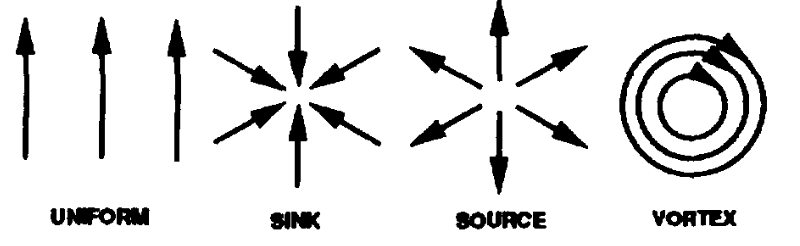
\includegraphics[width = .8\linewidth]{aerodynamics-primitives-Wejchert1991.png}
%     % 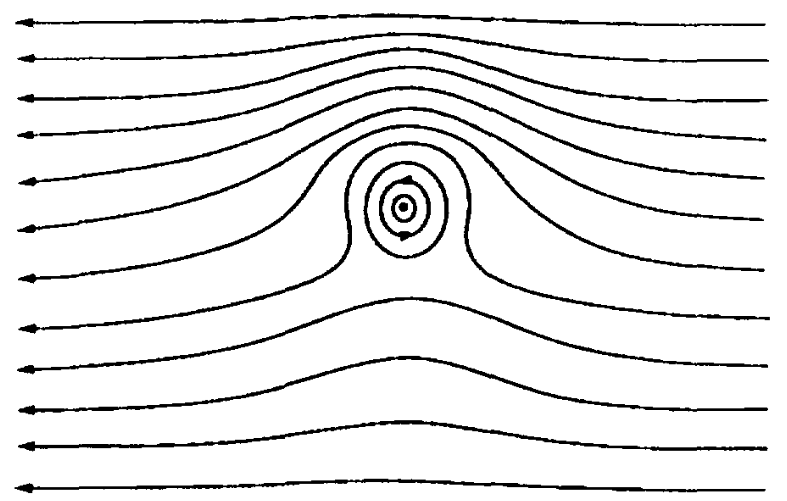
\includegraphics[width = .15\linewidth]{aerodynamics-addition-Wejchert1991.png}
%     \caption{\cite{Wejchert1991} propose to describe the flowfield of the environment by a combination of primitives, resulting in a simulation of wind field controllable by the user at very small memory cost. }
%     \label{fig:env-obj-wejchert-flow}
% \end{figure}

% \begin{figure}
%     \autofitgraphics[]{riverscape-primitives-Peytavie2019.png, riverscape-result-Peytavie2019.png}
%     \caption{\cite{Peytavie2019} uses a sparse representation of a river surface to include details at the water surface.}
%     \label{fig:env-obj-peytavie-river-primitives}
% \end{figure}

\AltTextImage{
    $\Wobj$ is a deformation field defined as the accumulation of flow primitives. The use of analytical primitives to represent localized variations within large-scale scenes has been explored in various contexts such as the edition of wind fields (\cite{Wejchert1991}, \cref{fig:env-obj-wejchert-flow}) and authoring of rivers' water surface geometry (\cite{Peytavie2019}, \cref{fig:env-obj-peytavie-river-primitives}). In the latter, flow primitives are primarily used to generate the geometry of the water surface, but the same primitives can also be reused to produce a flow field, enabling effects such as floating debris or leaves drifting along the surface. Because geometry is sensitive to overlapping influences, the authors. organize primitives into a blending tree, where merge and replace operations control how individual contributions interact. 
}{riverscape-primitives-Peytavie2019.png, riverscape-result-Peytavie2019.png}{\cite{Peytavie2019} uses a sparse representation of a river surface to include details at the water surface.}{fig:env-obj-peytavie-river-primitives}
\AltTextImage{
    On the other hand, \cite{Wejchert1991} showed that simply summing flow primitives generates velocity fields that approximate Navier-Stokes dynamics. Because their method affects motion rather than visible geometry, this additive approach offers a good trade-off between plausibility, user control and computation time.

    In our method, we adopt a similar additive approach to combine Kelvinlet-based primitives. Our goal is to define a deformation field and as such, summation offers an effective and intuitive way to accumulate the influence of multiple localized deformations at various scales, without requiring additional structure to resolve overlaps.
}{aerodynamics-primitives-Wejchert1991.png, aerodynamics-addition-Wejchert1991.png}{\cite{Wejchert1991} propose to describe the flowfield of the environment by a combination of primitives, resulting in a simulation of wind field controllable by the user at very small memory cost.}{fig:env-obj-wejchert-flow}
% To model the localized influence of environment objects on water currents, we adopt Kelvinlets, a family of closed-form, continuous deformation functions derived from the fundamental solutions to the equations of linear elasticity in an infinite medium.


% \begin{figure}
%     \autofitgraphics[]{kelvinlets-grab-demo-DeGoes2017.png, kelvinlets-demo-DeGoes2017.png}
%     \caption{\cite{DeGoes2017} presents four types of deformations using Kelvinets, resulting in organic pinch-like interaction with the original field. From left to right: a grab on a \textcopyright Disney/Pixar character, a twist, a scale and a pinch operation. }
%     \label{fig:env-obj-kelvinlets-demo}
% \end{figure}

Kelvinlets were introduced to computer graphics as an efficient means of producing physically plausible and interactive deformations \cite{DeGoes2017}. In our context, they provide a smooth and compact representation of flow alterations, ideal for integrating environmental features into vector field modeling.

Kelvinlets are based on the Kelvin solution, which is the Green's function of the Navier-Cauchy equations of linear elasticity. It describes the displacement $\tensor{u}(\p)$ at a point $\p \in \R^3$ caused by a force applied at $\q$, in an isotropic, homogeneous elastic material:
\begin{align}
    \mu \nabla^2 \tensor{u} + (\lambda + \mu) \nabla(\nabla \cdot \tensor{u}) + \delta(\p - \q) \force = 0
\end{align}
where $\lambda$ and $\mu$ are the Lamé parameters, with $\mu$ also known as the shear modulus, and $\force$ is the force vector applied at a single point $\q$ via the Dirac delta function $\delta(\p - \q)$.

\AltTextImage{
    To regularize the singularity at $\p = \q$, \cite{DeGoes2017} introduced a smoothed form known as the regularized Kelvinlets, which allow deformation effects to fall off smoothly with distance, and prevent numerical instabilities.

    Given a center $\q$, an evaluation point $\p$, and a regularization $\eps$, we define $\tensor{r} = \p - \q$ and the regularized distand $r_{\eps} = \sqrt{\|\tensor{r}\|^2 + \eps^2}$.

    We use the scale and grab formulations of the regularized Kelvinlets brushes (\cref{fig:env-obj-kelvinlets-demo}), denoted as $s_\eps(\tensor{r})$ and $g_\eps(\tensor{r})$ respectively to simulate obstruction and diversion, are defined as
    \begin{align*}
        s_\eps(\tensor{r}) &= (2b - a) \left( \frac{1}{r_\eps^3} + \frac{1}{2r_\eps^5} \right)(s \tensor{r}) \\
        g_\eps(\tensor{r}) &= \left[ \frac{a - b}{r_\eps} \identity + \frac{b}{r_\eps^3} \tensor{r} \tensor{r}^t + 
    \frac{a \eps^2}{2 r_\eps^3} \identity \right] \force
    \end{align*}
    with $a = \frac{1}{4 \pi \mu}$ and $b = \frac{a}{4 (1 - \upsilon)}$ provided $\mu$ a shear modulus and $\upsilon$ a Poisson ratio provided for each Kelvinlet, $s$ a scaling factor and $\force$ the force vector of the grab operation. These values are tunable per object to simulate different material or flow resistance behaviors.
}{kelvinlets-grab-demo-DeGoes2017.png, kelvinlets-demo-DeGoes2017.png}{\cite{DeGoes2017} presents four types of deformations using Kelvinets, resulting in organic pinch-like interaction with the original field. Top: a grab on a \textcopyright Disney/Pixar character. From left to right: a twist, a scale and a pinch operation. }{fig:env-obj-kelvinlets-demo}

Deformations defined on curves use $\q = \closestCp$ with $\closestCp$ the closest point on the curve from the point $\p$ and $\force = C'(\p)$. We can then define $\tensor{u}_o(\p) = s_\eps(\q - \p) + g_\eps(\p - \q)$.
Finally, we can retrieve the velocity field from the objects, with a per-object coefficient $\lambda_o$ for the strength of its flow effects (due to its size, porosity, surface roughness, ...):
\begin{align}
    \Wobj(\p) = \sum_{o \in \objects}^{}{\lambda_o \tensor{u}_o(\p)}
\end{align}

The use of regularized Kelvinlets is well-suited to our model. They offer a compact representation thanks to their closed-form definition, which allows each deformation to be described analytically without the need for precomputed data or large simulation grids. They maintain continuity, ensuring that the resulting vector field is smooth and free of visual or numerical artifacts, which is crucial when blending influences from multiple environment objects. Their behavior is physically plausible, as they are derived from fundamental solutions to elasticity equations, and can convincingly simulate natural flow behaviors such as deflection around obstacles or local flow obstruction. They are also computationally efficient, since their evaluation is lightweight and independent of the size or complexity of the terrain, making them particularly suitable for integration into large-scale procedural generation pipelines and real-time interactive applications.


\subsection{Environment stability}
\begin{figure}[H]
    \centering
    \autofitgraphics[]{diffusion_no_decay_no_wind.pdf, diffusion_decay_0-05_no_wind.pdf}
    % 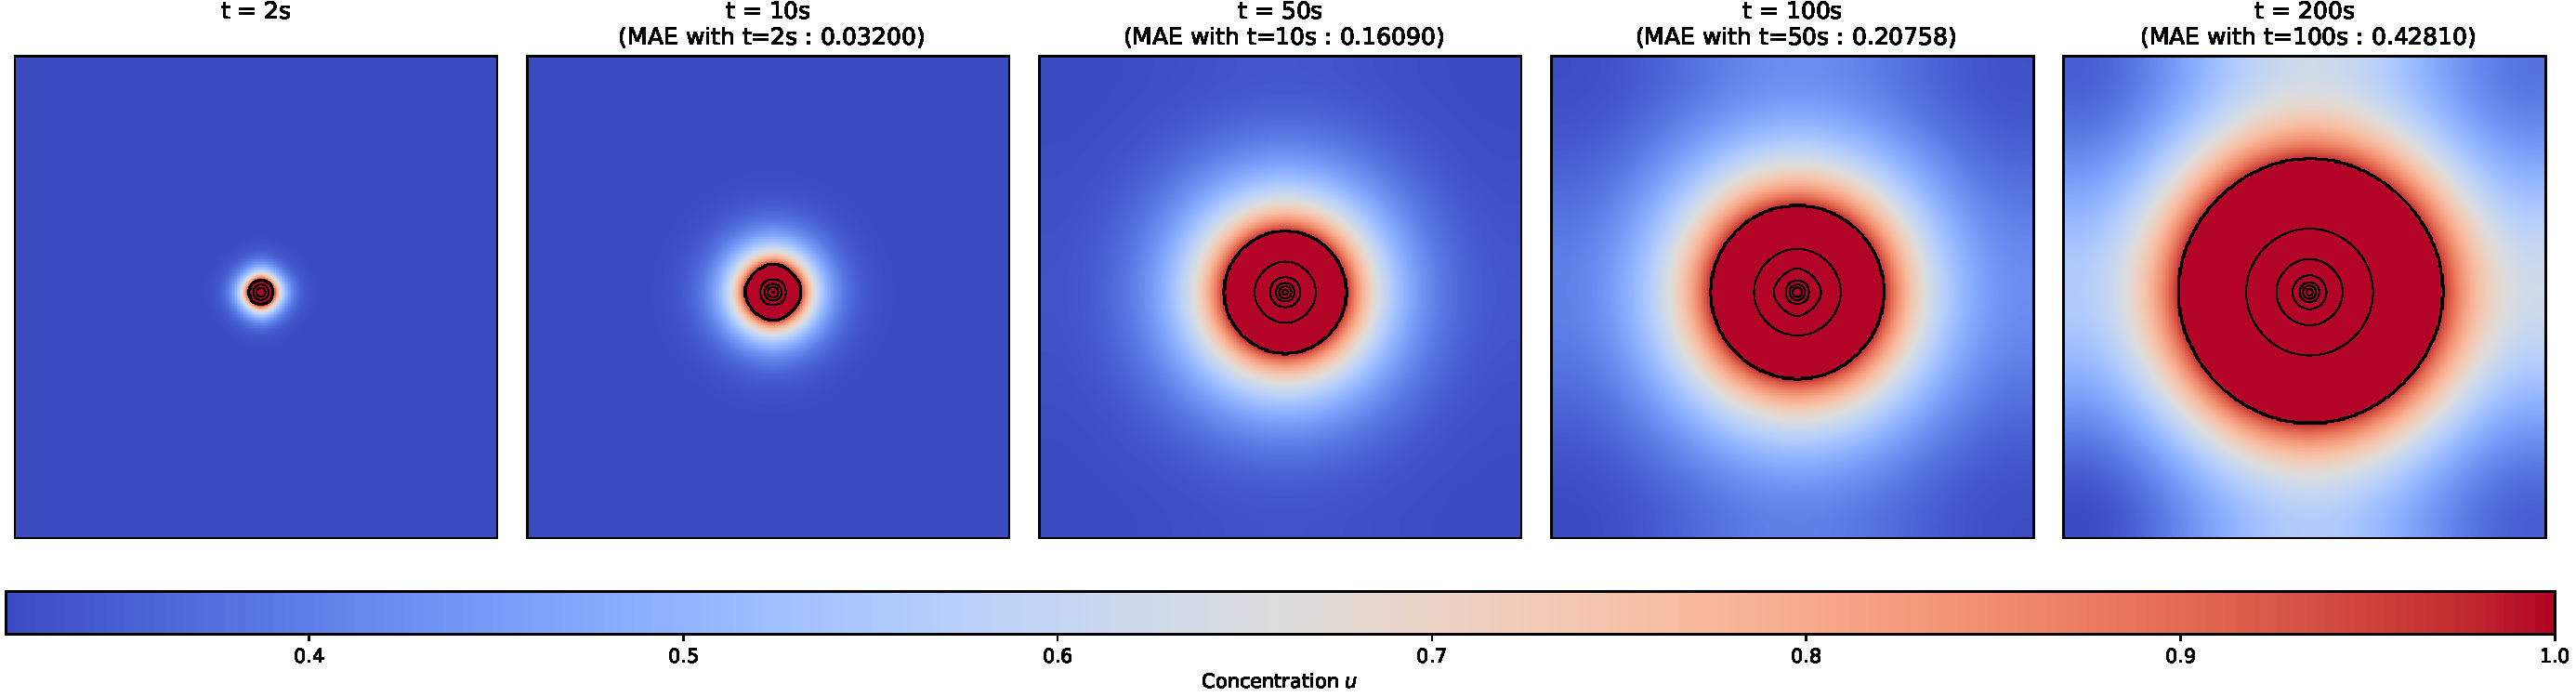
\includegraphics[width=.45\linewidth]{diffusion_no_decay_no_wind.pdf}
    % 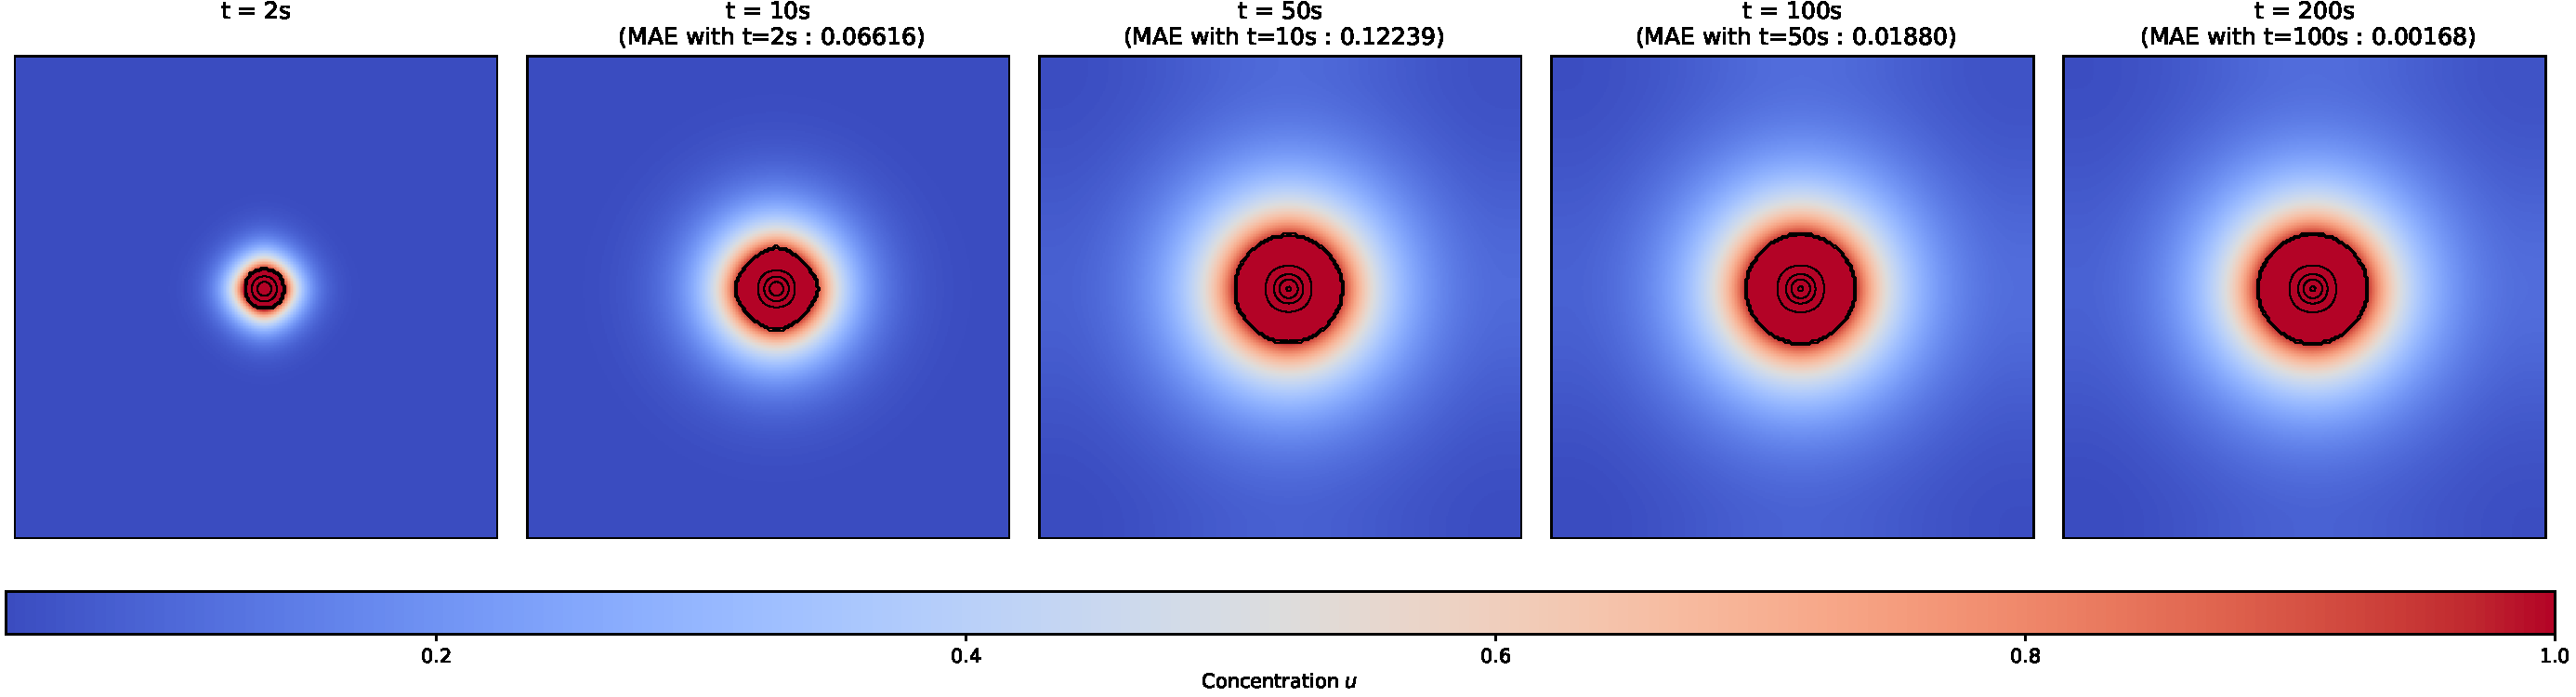
\includegraphics[width=.45\linewidth]{diffusion_decay_0-05_no_wind.pdf}
    % \autofitgraphics[]{diffusion_no_decay_linear_wind.pdf, diffusion_decay_0-05_linear_wind.pdf}
    % 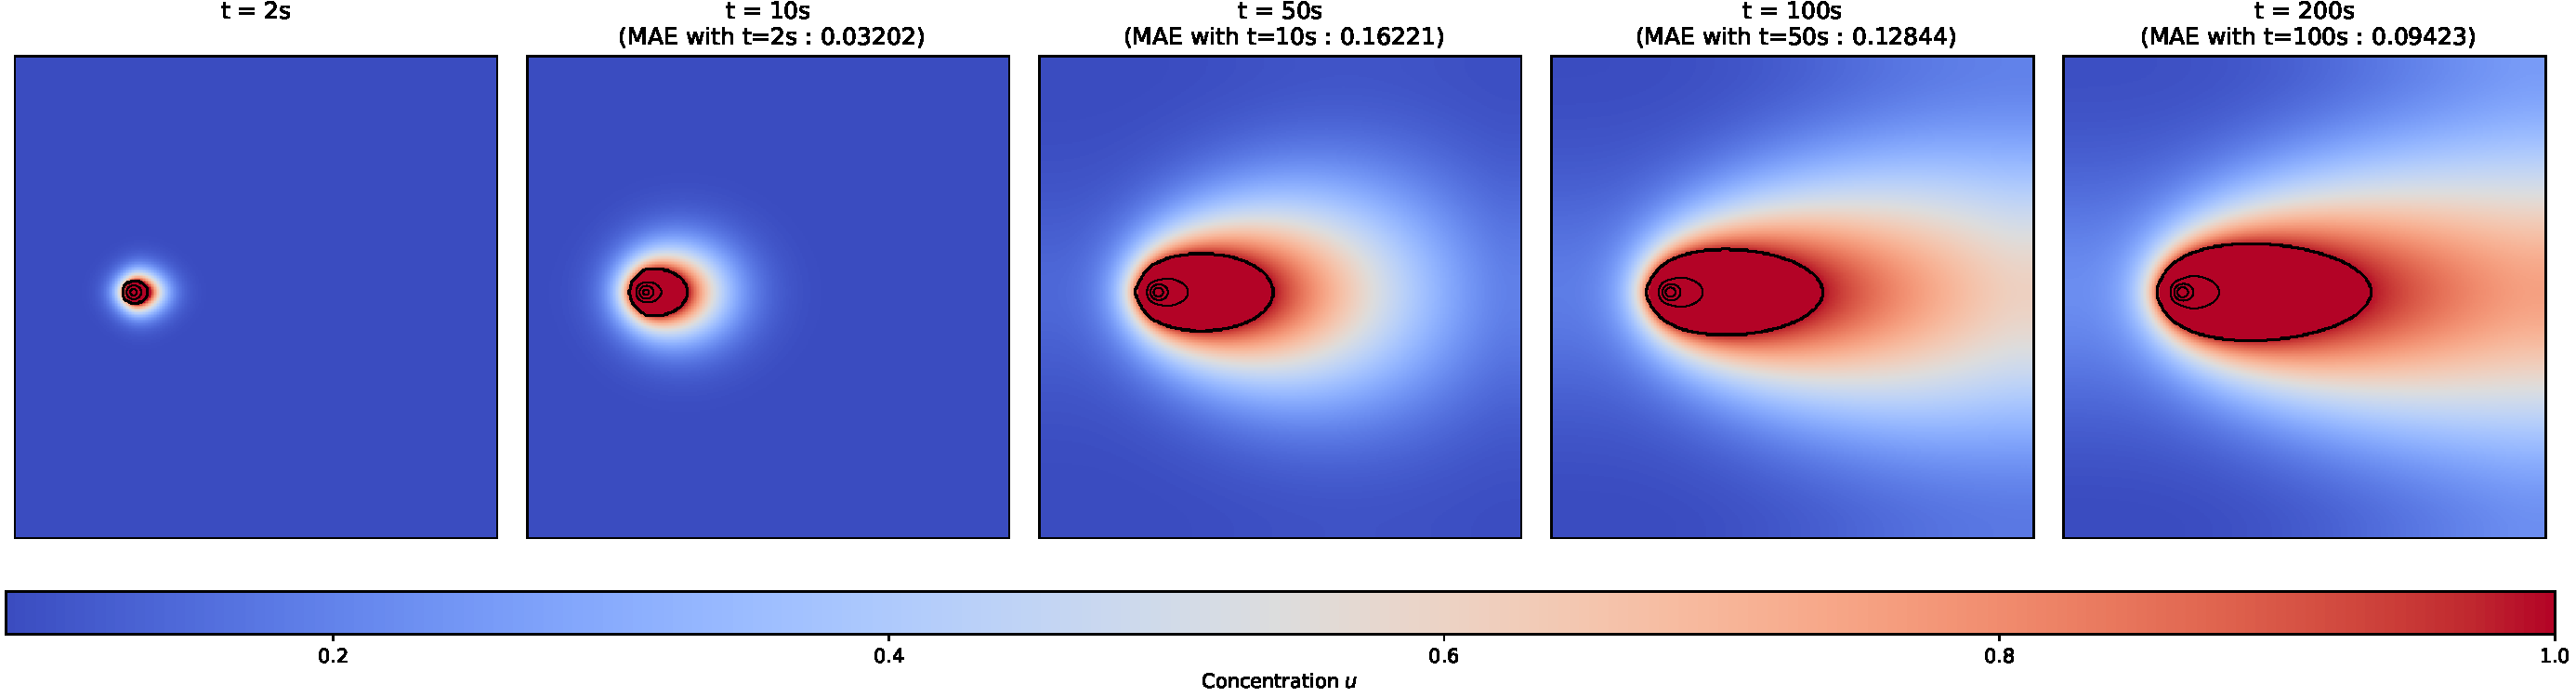
\includegraphics[width=.45\linewidth]{diffusion_no_decay_linear_wind.pdf}
    % 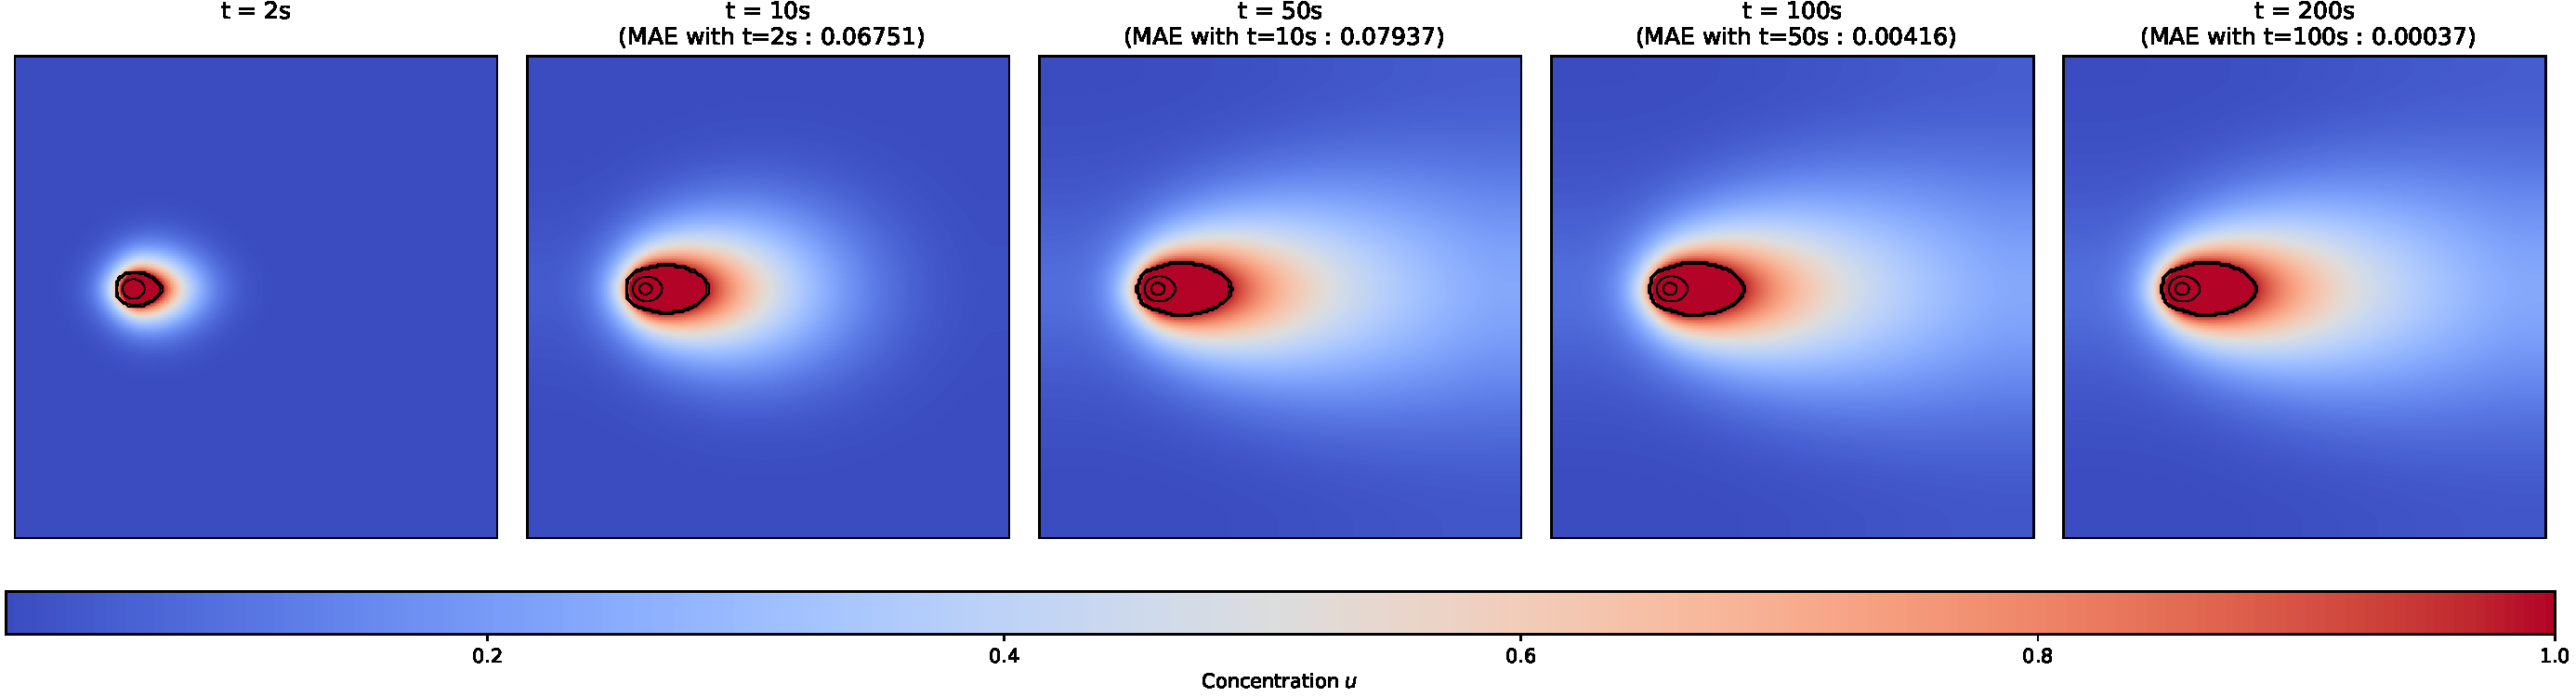
\includegraphics[width=.45\linewidth]{diffusion_decay_0-05_linear_wind.pdf}
    \autofitgraphics[]{diffusion_no_decay_circular_wind.pdf, diffusion_decay_0-05_circular_wind.pdf}
    % 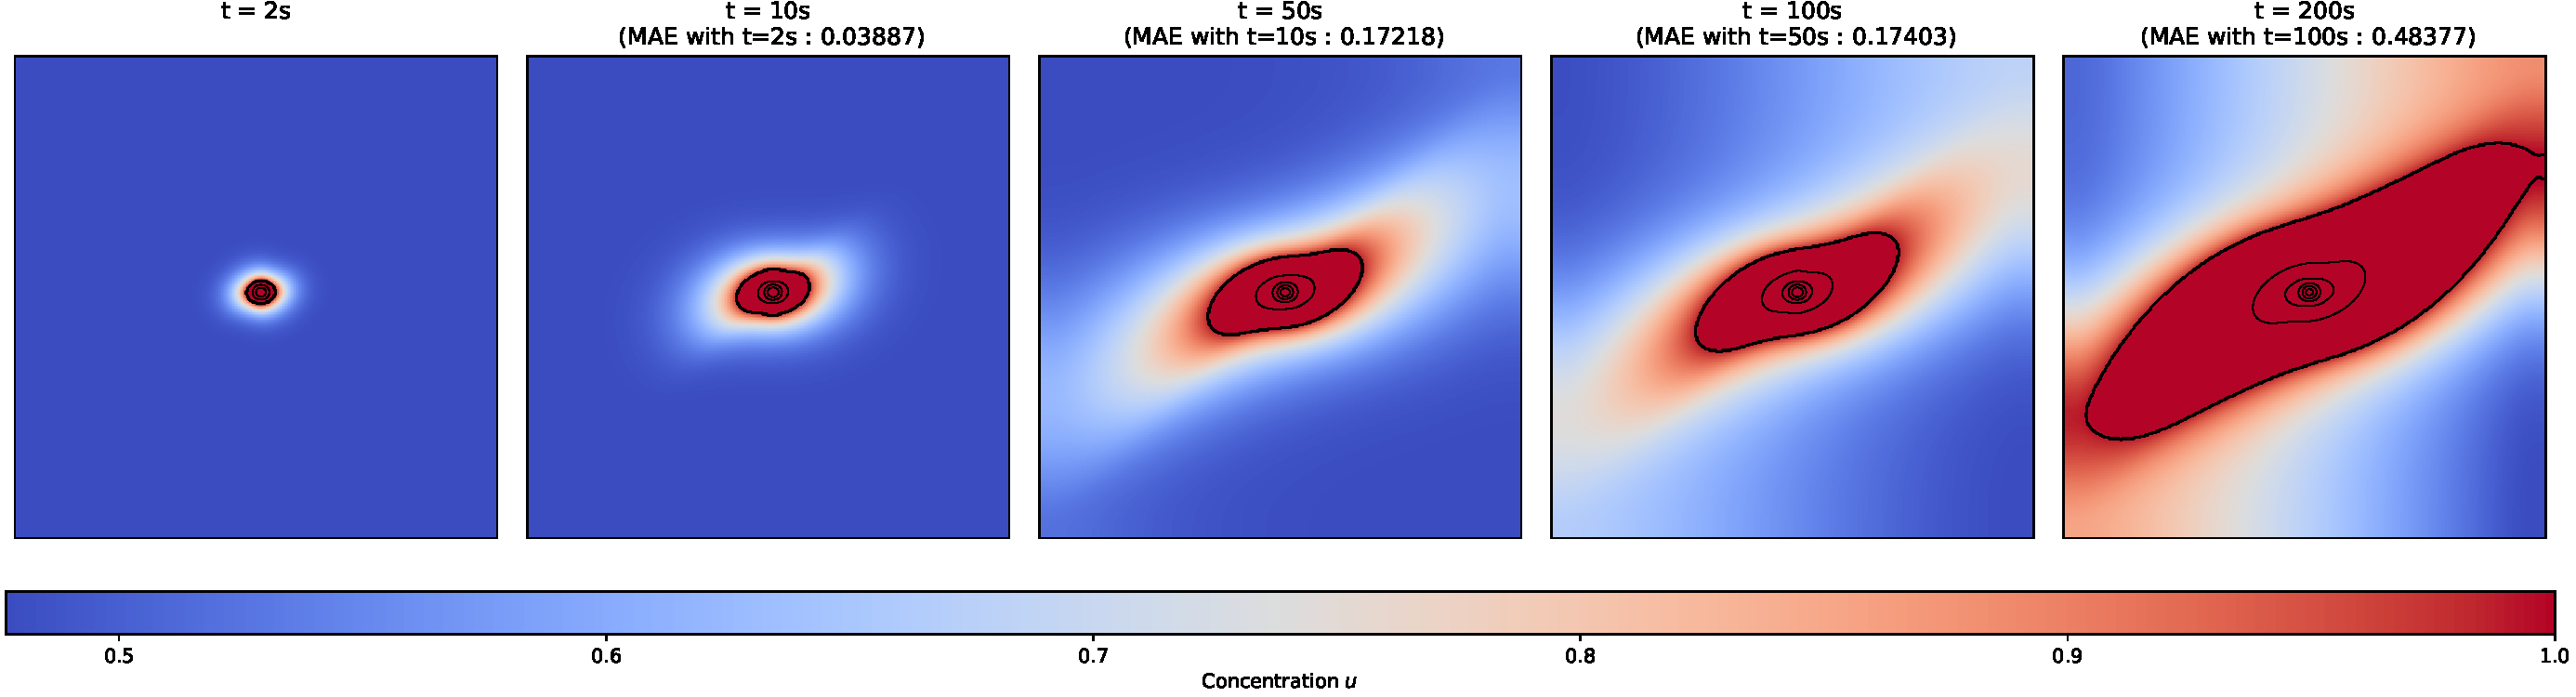
\includegraphics[width=.45\linewidth]{diffusion_no_decay_circular_wind.pdf}
    % 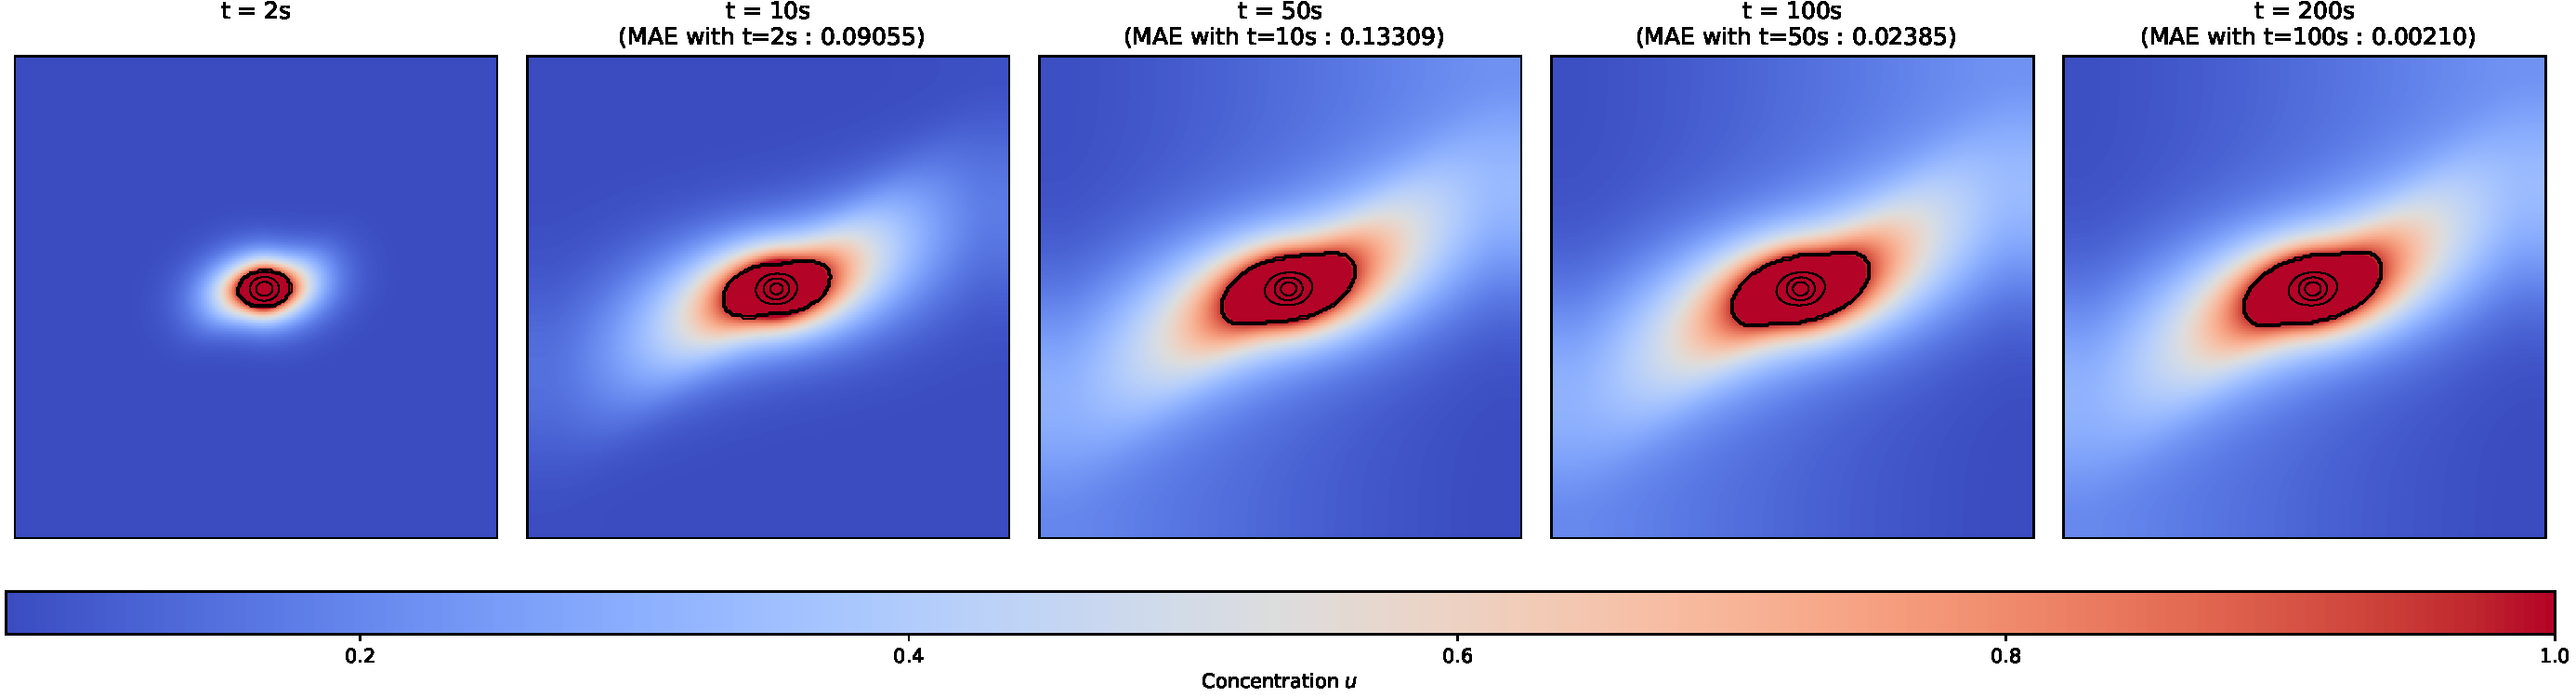
\includegraphics[width=.45\linewidth]{diffusion_decay_0-05_circular_wind.pdf} 
    \caption{The addition of a decay term in the advection-diffusion-reaction equation, the spread of the \glosses{EnvMat} tends to a stability after few iterations (right) while the total mass would constantly increase without decay (left) (concentration value is clamped to 1 for visual purposes). This is also true when a flow field is present (bottom). Moreover, thanks to the decay, we see less instabilities regarding the boundary conditions (bottom left uses a zero-gradient boundary condition, resulting in a simulation explosion from the borders). }
    \label{fig:env-obj-stability-examples}
\end{figure}

\Glosses{EnvObj} and \glosses{EnvMat} are inspired by the ecological concept of biogeocoenosis, which describes the relationship between living organisms (biotic) and their non-living environment (abiotic). These interactions closely mirror the processes observed in natural ecosystems, where biotic and abiotic components continuously influence each other, leading to a balanced and stable environment. Gubanov and Degermendzhy [CITATION] describe biogeocoenosis as almost-closed systems, with many parallels possible with thermodynamics such as the concept of dynamic equilibrium. In a biogeocoenosis, the various processes, such as the spread of nutrients, the growth of vegetation, or the erosion of soil, tend toward a state of balance. 

Similarly, in our method, the interaction between \glosses{EnvObj} and \glosses{EnvMat} is modeled using a reaction-diffusion-advection framework. This model captures how \glosses{EnvMat} are spread and absorbed within the terrain. Thanks to the decay rate of the \glosses{EnvMat}, the system progresses toward a dynamic equilibrium, where the distribution of \glosses{EnvMat} stabilizes. This stabilization reflects a state of balance where the rates of spreading and absorption and decay are equal, and the \glosses{EnvVal} become coherent across the landscape. For example, a river might spread sediments downstream, which are gradually absorbed by the surrounding terrain, leading to a stable sediment distribution over time. Similarly, moisture emitted by a forest will eventually reach a balance with the surrounding soil and atmosphere, creating a stable, humid environment.

The only factor that can disrupt this equilibrium is a change in the \glosses{EnvVal}. Changes such as an increase in temperature, a shift in wind patterns, or the introduction of a new \gloss{EnvObj} can alter the balance, leading to a new phase of interaction and stabilization.


\section{User interactions}
\label{sec:env-obj-interaction}
The user can guide the generation process. The use of simple shapes as \glosses{EnvObj} facilitate the edition of the simulation, as we can interactively add, remove or modify \glosses{EnvObj}, or focus the generation process in a restricted area. Interaction with the \glosses{EnvVal} is also provided as \glosses{GeoEvent}, that the user can invoke during the simulation. While the direct interactions on the \glosses{EnvObj} are instantaneous, as a the \glosses{GeoEvent} are active on a given duration.

\subsection{Direct interactions with the \glosses{EnvObj}}
\label{sec:env-obj-manual-interaction}
The interactive nature of our simulation enables the user to modify the state of the terrain by manipulating directly the \glosses{EnvObj} of the scene. We assume the modifications applied between two iterations of the simulation.

Translating an \gloss{EnvObj} is trivial, we simply requires to evaluate the state of the \glosses{EnvObj} at a translated position. The deformation of \glosses{EnvObj} can be applied on curve and region \glosses{EnvObj} by updating the control points of the skeleton and recomputing the resulting implicit surfaces. The evaluation positions used for region \glosses{EnvObj} are displaced by applying a cage deformation of the 2D shape using the Green coordinates of points in the shape. After the alteration of the region, evaluation points should be keeping a similar distribution than before, avoiding unexpected results during the interaction.
By modifying an \gloss{EnvObj}, the \glosses{EnvVal} may change, which can result in the destruction of the now incompatible environment objects in the scene (\cref{fig:env-obj-user-interaction}).

\begin{figure}
    % \centering
    \autofitgraphics[]{InteractionEdition1.png, InteractionEdition2.png, InteractionEdition3.png}
    % 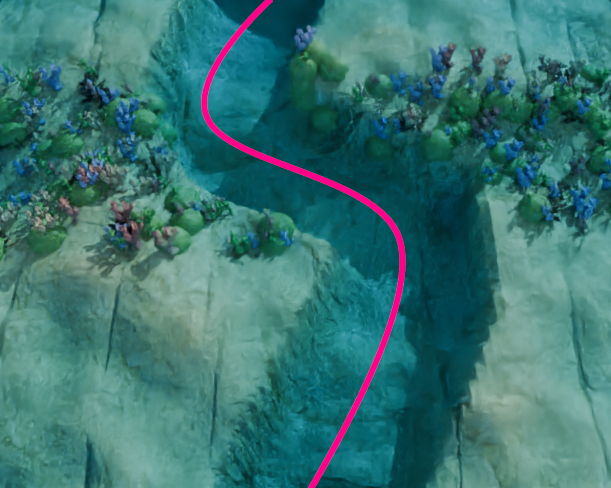
\includegraphics[width = 0.3 \linewidth]{InteractionEdition1.png}
    % 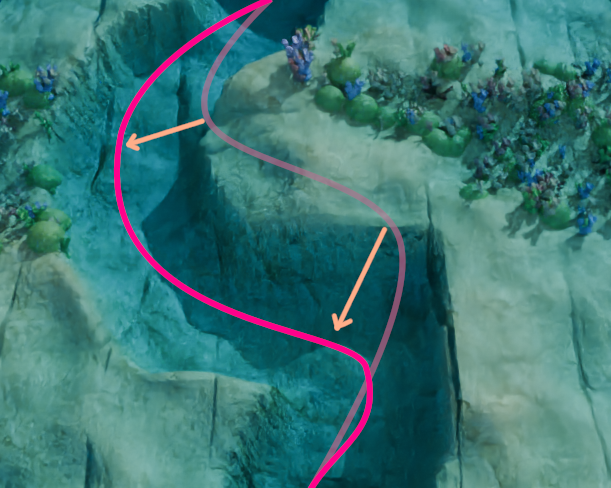
\includegraphics[width = 0.3 \linewidth]{InteractionEdition2.png}
    % 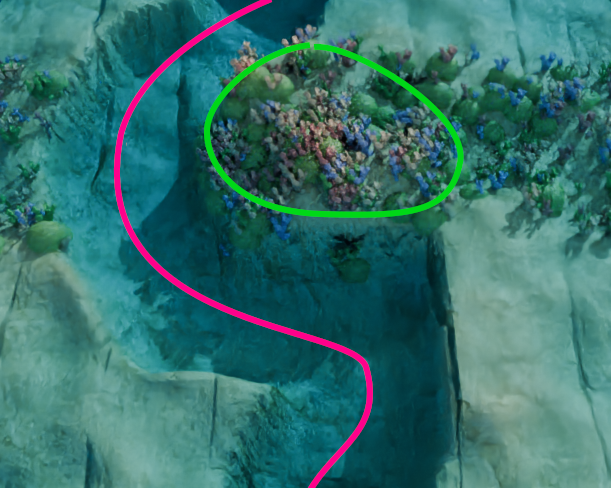
\includegraphics[width = 0.3 \linewidth]{InteractionEdition3.png}
    \caption{Starting from a coral colony developed around a canyon (\textit{left}), the user edits the shape of the canyon, resulting in a different configuration of the scene, killing the corals that ends too deep in the water (\textit{center}) and the development and growth of new corals at the previous location of the canyon (\textit{right}). }
    \label{fig:env-obj-user-interaction}
\end{figure}

As long as a non-zero \gloss{FitnessFunc} is defined in the terrain, new \glosses{EnvObj} can be forced by the user at any point of the simulation. 

% \subsection{Guiding the simulation}
Control over the region of the terrain that should be updated can be given by adjusting all \glosses{FitnessFunc} through a scalar field $\influence: \R^2 \to \R $ such that the \gloss{FitnessFunc} $\fitnessFunc(\p)$ of any new \gloss{EnvObj} is evaluated as $\fitnessFunc^*(\p) = \influence{\p} \fitnessFunc(\p)$. This is especially useful in the planning of robotic simulations as we can first generate the overall shape of our terrain and secondly focus the generation process around the areas that may be visited by the robot, avoiding useless simulations and computer power. 
\cref{fig:env-obj-coral-colonization-scene} shows an example of colonization of the coral polyps that we limited manually into an annulus.
% \cref{fig:env-obj-focus-area-example} shows an example of colonization of the coral polyps that we limited manually.

% \begin{figure}
%     % \centering
%     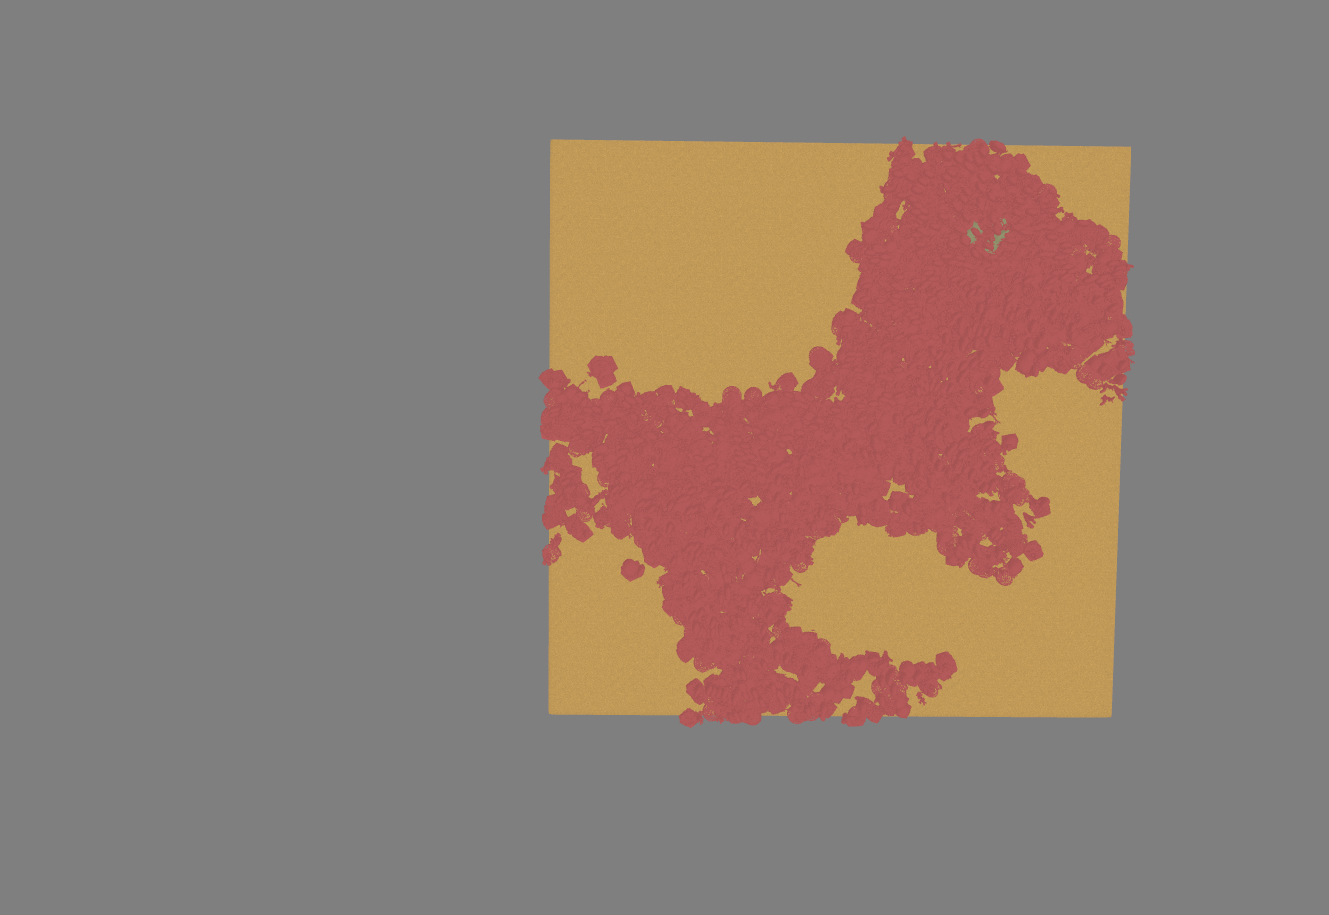
\includegraphics{guidedGeneration1.png}
%     \caption{Controlling the generation area can produce a user-defined focused shape.}
%     \label{fig:env-obj-focus-area-example}
% \end{figure}

% - Changing the water currents

Our water current simulation is modeled as a simple vector field. As such, the user is able to interact with it at any moment of the simulation, allowing for the death of sensible \glosses{EnvObj} while it will guide the simulation into a new landscape. By modifying the water currents, the user also modifies the transport rate of \glosses{EnvMat} at this position. The modification of currents is given as a stroke, a parametric curve $\curve$ for which we evaluate $\Delta \Wuser(\p)$ just as for curved environment objects (\cref{sec:env-obj-water-currents}).

\subsection{Indirect interaction with \glosses{EnvObj}}
\label{sec:env-obj-events}
A configuration file can define in advance the different \glosses{GeoEvent} that should be triggered during the simulation. This can be useful to generate landscapes that are close to some existing locations. 
Multiple \glosses{GeoEvent} can be triggered either as sudden or continuous environmental changes. These changes play a huge role in the morphology of landscapes.
We define \glosses{GeoEvent} with a starting point and an ending point, such that at any time of the simulation we can compute the progress of the \gloss{GeoEvent} as $\tEvent \in [0, 1]$.

Water level changes are important \glosses{GeoEvent} that shape the underwater landscapes. As previously submerged \glosses{EnvObj} get elevated above water level, flora and fauna terrain features dry and die. Deprived from the living part of the features, everything is more affected by terrestrial erosion. By updating the value of the depth $\depth$ evaluated in the \glosses{FitnessFunc}, any \gloss{EnvObj} that is sensible to the depth will be impacted automatically, that may be causing death (\cref{fig:env-obj-water-event}). The modification of the water level is defined as 
\begin{align*}
    \depth(\p) = \depth_0(\p) + \sum_{e \in \events} \Delta \depth_e \tEvent
\end{align*}
with $\Delta \depth_e$ the amount of water rising or lowering during an \gloss{GeoEvent}. We assumed a linear evolution of the water level during an \gloss{GeoEvent}. This allows to evaluate the depth at any point in space and in time.

\begin{figure}
    % \centering
    \autofitgraphics[]{InteractionWater1.png, InteractionWater3.png}
    % 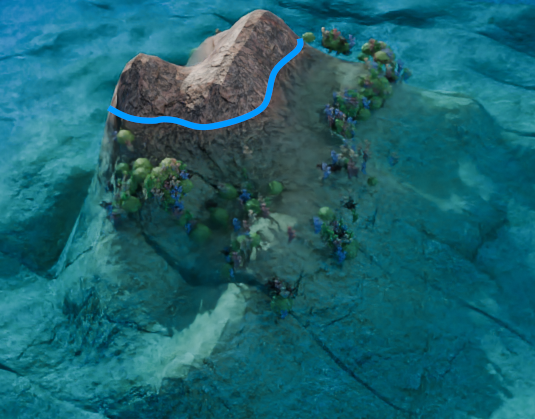
\includegraphics[width = 0.45 \linewidth]{InteractionWater1.png}
    % 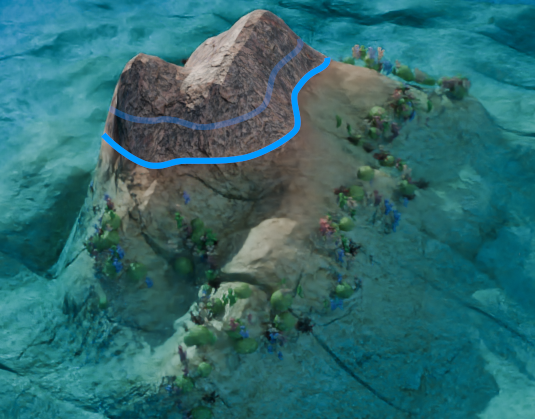
\includegraphics[width = 0.45 \linewidth]{InteractionWater3.png}
    \caption{Lowering the water level by a few meters caused most of the coral objects to satisfy $\fitnessFunc \leq 0$, causing their death. Since the water level (blue) decrease slowly, new coral objects spawn progressively at a lower altitude.}
    \label{fig:env-obj-water-event}
\end{figure}

Subsidence and uplift are the main \glosses{GeoEvent} that create or destroy islands in the long term. These \glosses{GeoEvent} are simulated as a simple factor on the height field of the generated terrain (\cref{fig:env-obj-subsidence-event}). Subsidence is not always uniform in the terrain. As such, the user can provide a position $\q$ at which the subsidence is the strongest, the amount of subsidence applied $\Delta \height_e$ and a standard deviation $\std$ for which we can then compute at any point in space and time of the simulation the height of the terrain
\begin{align*}
    \height(\p) = \height_0(\p) \cdot \sum_{e \in \events}{G(\norm{\p - \q})} \Delta \height_e \tEvent 
\end{align*}
with $G(x)$ the Gaussian function
\begin{align*}
    G(x) = \frac{1}{\std \sqrt{2\pi}} \exp \left(-\frac {x^{2}}{2 \std ^{2}}\right)
\end{align*}

\begin{figure}
    % \centering
    \autofitgraphics[]{InteractionSubsidence1.png, InteractionSubsidence2.png}
    % 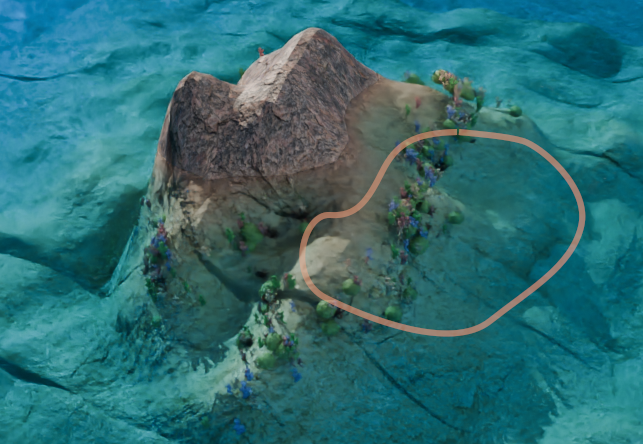
\includegraphics[width = 0.45 \linewidth]{InteractionSubsidence1.png}
    % 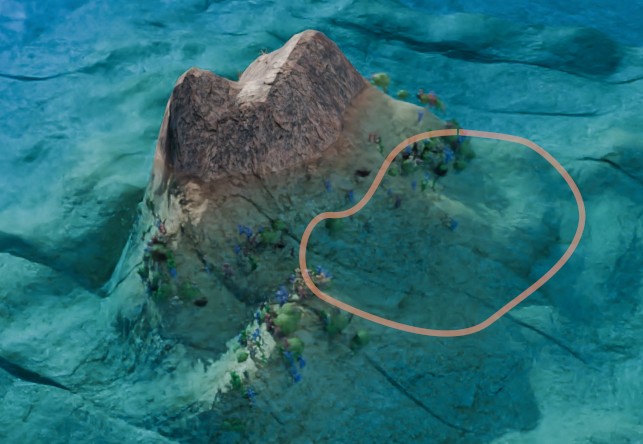
\includegraphics[width = 0.45 \linewidth]{InteractionSubsidence2.png}
    \caption{Simulating subsidence on a part of the terrain (brown area) cause the depth value to change locally, resulting in the death of coral objects that find themselves too deep to survive. Here two subsidence \glosses{GeoEvent} are triggered in parallel. }
    \label{fig:env-obj-subsidence-event}
\end{figure}

Storms are factors of the geomorphology of coral reefs \cite{VilaConcejo2016, Oron2023} and coasts \cite{Dominguez2005, Cowart2010}. Due to the extreme wind and wave velocities coasts are highly eroded in a short time period and the more fragile corals near the water surface are broken, possibly causing breaches in the reefs and spreading polyps in the currents direction. While there are many factors at play to understand the apparition of storms and the hydrodynamics affecting it, we simplified the model of storms to the user as a single epicenter $\q$ with a wind velocity $\windVelocity$ and a standard deviation $\std$ representing the spread around the epicenter (\cref{fig:env-obj-storm-event}). The computation of water currents are then computed as 
\begin{align*}
    \Wuser(\p) = \Wuser^*(\p) + \sum_{e \in \events} {\windVelocity G(\norm{\p - \q})}
\end{align*}
In this case, we did not include the linear factor $\tEvent$ as storms are usually conserving a constant force for the time of the few weeks or months of their occurrence. 

\begin{figure}
    % \centering
    \autofitgraphics[]{interactionStorm1.png, interactionStorm2.png}
    % 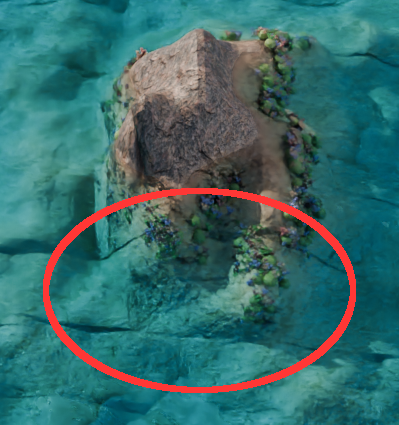
\includegraphics[width = 0.45 \linewidth]{interactionStorm1.png}
    % 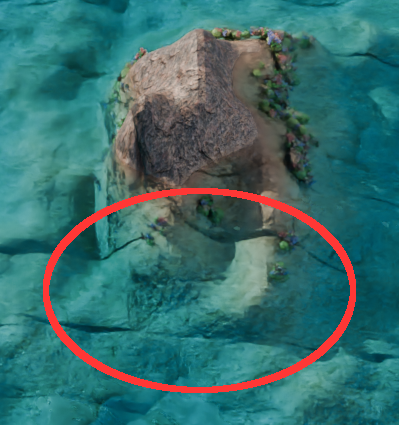
\includegraphics[width = 0.45 \linewidth]{interactionStorm2.png}
    \caption{The result of a storm localized on one side of the island (red area) modifies the result of the evaluation of \glosses{EnvObj} around its epicenter for a short period of time. Most of the coral objects died from the \gloss{GeoEvent}, except few \glosses{EnvObj} less sensible to water currents strength. }
    \label{fig:env-obj-storm-event}
\end{figure}

% Just as for the rise and lowering of water level, the heat is modeled as a simple value of the environment. For shallow areas (<100m) we assume a linear relation between depth and temperature, and a constant value for the terrestrial environment. As such, we can model a heat wave by a change of the \glosses{EnvVal}. \Glosses{EnvObj} who are sensible to temperature may die instantly. The modification of the temperature is defined as 
% \begin{align*}
%     \temperature(\p) = T_0(\p) + \sum_{e \in \events} \Delta \temperature_e \tEvent + c \depth(\p)
% \end{align*}
with $\Delta \temperature_e$ the change of heat during an \gloss{GeoEvent}, $\temperature_0$ the temperature at the water surface, and $c$ a very small factor.

The framework can easily be extended as the \gloss{GeoEvent} system stays similar for all \glosses{GeoEvent}. Including higher level simulations in the \gloss{GeoEvent} system can be added, such as the simulation of tectonic activity, the use of fluid dynamics for tsunami \glosses{GeoEvent}, the integration of human activity, ...

\section{Results and discussion}
\label{sec:env-obj-results}
Our method provides a way to generate scenes at different scales. We demonstrate this capacity with the generation of a large scene of an island (\cref{fig:env-obj-teaser}) after what we focused the generation process in a canyon (\cref{fig:env-obj-canyon-scene}), then a small-scale visualization of coral colonies (\cref{fig:env-obj-coral-colonization-scene}).
In the examples, we rendered the \glosses{EnvObj} as a implicit tree or as individual meshes. The island, lagoons, reefs, canyons and sand ripples as implicit surfaces

% \subsection{Mid-scale}
% \label{sec:env-obj-mid-scale}
A canyon scene can be generated using our method. The water flow is affected by the curve of the canyon such that the currents are oriented in the direction of the curve's tangent.In this example, we force the position of arches to be inside the canyon. The arches deposits a material "rock deposit", which is the main element of the \gloss{FitnessFunc} of the Rock object. The "rock deposit" is slightly affected by water currents, but its mass make it highly affected by gravity. As such, rocks will spawn underneath arches. In reality, an arch is often created as part of a large coral boulder that sees the calcareous bottom part detached by the water currents, often resulting in an arch surrounded by big rocks and smaller rocks from the erosion of the first rocks.
As such, we define an \gloss{EnvObj} "Arch" with a \gloss{FitnessFunc} $\fitnessFunc_{arch}(\p) = 5 - d(canyon - \p) * \norm{\Water(\p)}$, an \gloss{EnvObj} "Rock" using $\fitnessFunc_{rock}(\p) = \material_{rock\_deposit}(\p)$ and Pebble using $\fitnessFunc_{pebble}(\p) = \material_{smaller\_rock\_deposit}(\p)$. Finally, sand ripples are simply described as curves appearing where there is a lot of sand available: $\fitnessFunc_{ripple}(\p) = \material_{sand}(\p)$.
Following these simple rules, \cref{fig:env-obj-canyon-scene} shows the emergence of details in the scene. 

% \subsection{Small-scale}
% \label{sec:env-obj-small-scale}
In this example we defined three different types of corals, coralA, coralB and coralC, to illustrate the possibility to model behaviours from the choice of \glosses{FitnessFunc}. Each of the coral types deposits a material "coral polyp" and "coral polyp A" ("coral polyp B" and "coral polyp C" respectively). By considering a \gloss{FitnessFunc} that minimize the ratio $\frac{\text{coral polyp}}{\text{coral polyp A}}$, we can see an emergent behavior of the three types of coral fighting for the space colonization.
\cref{fig:env-obj-coral-colonization-scene} shows the result of this simulation at three different interations. At the border between two colonies, none of the colonies make progression due to the amount of coral polyp specific from the other colony.

\begin{figure*}
    % \centering
    \autofitgraphics[]{col0.png, col1.png, col2.png, col3.png}
    % 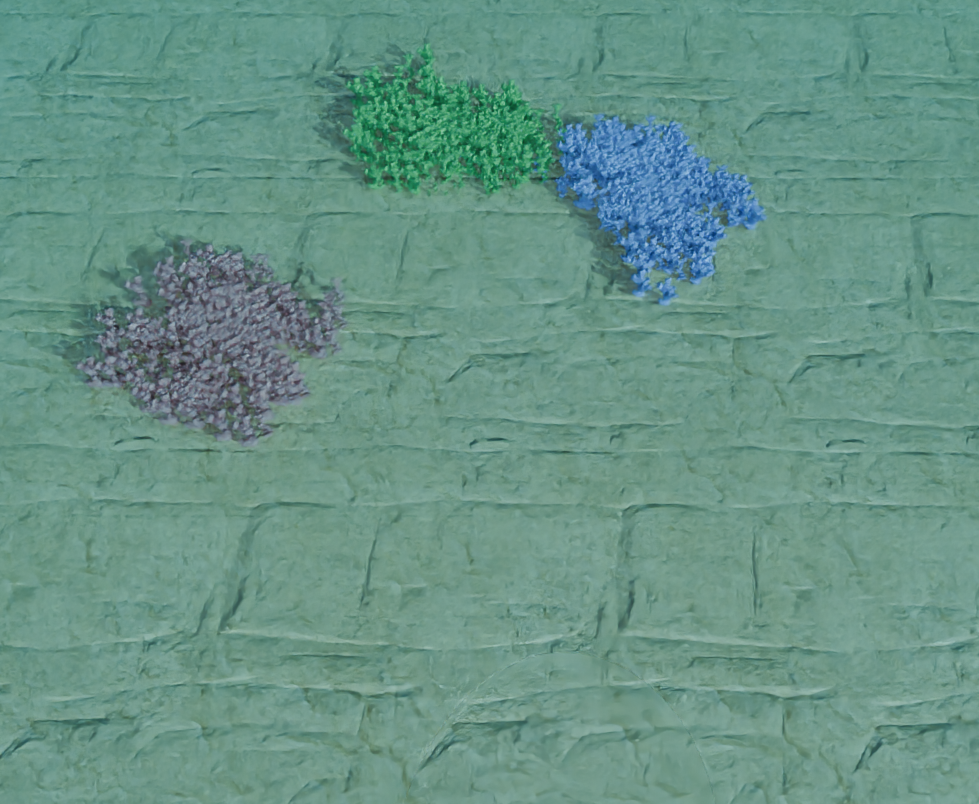
\includegraphics[width=0.24 \linewidth]{col0.png}
    % 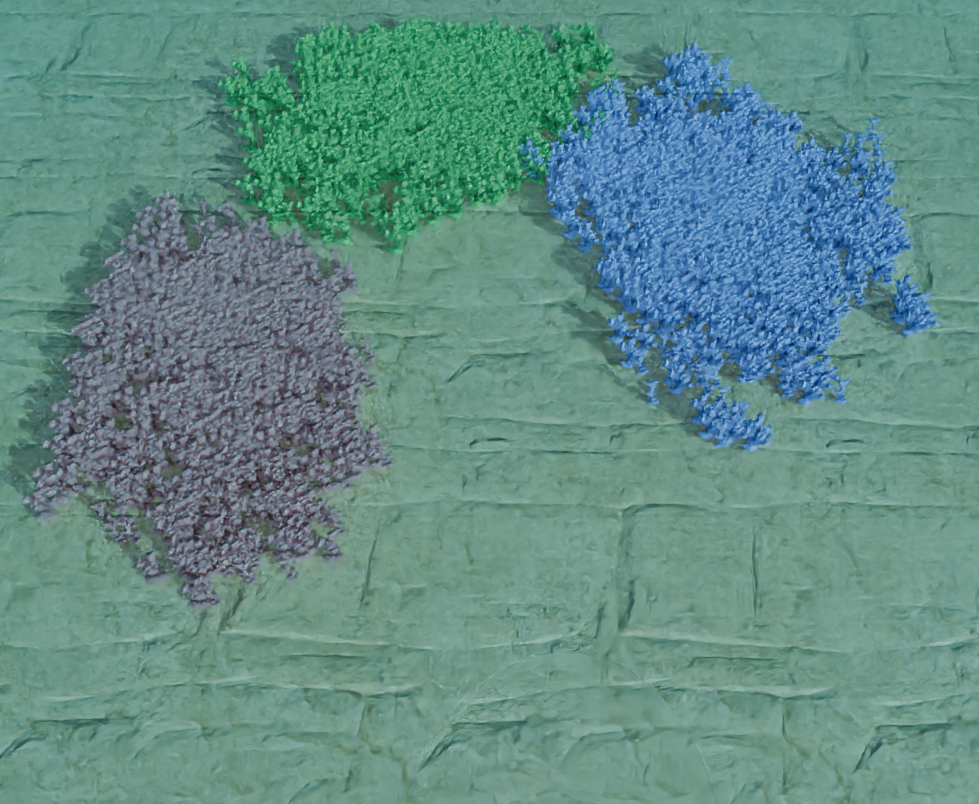
\includegraphics[width=0.24 \linewidth]{col1.png}
    % 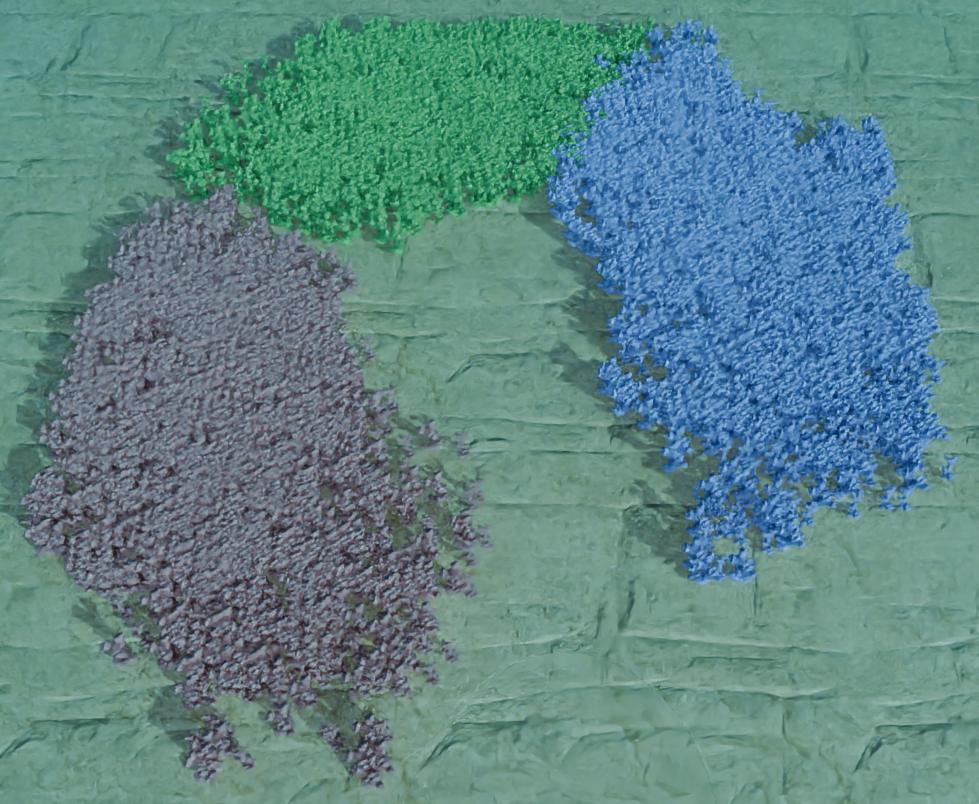
\includegraphics[width=0.24 \linewidth]{col2.png}
    % 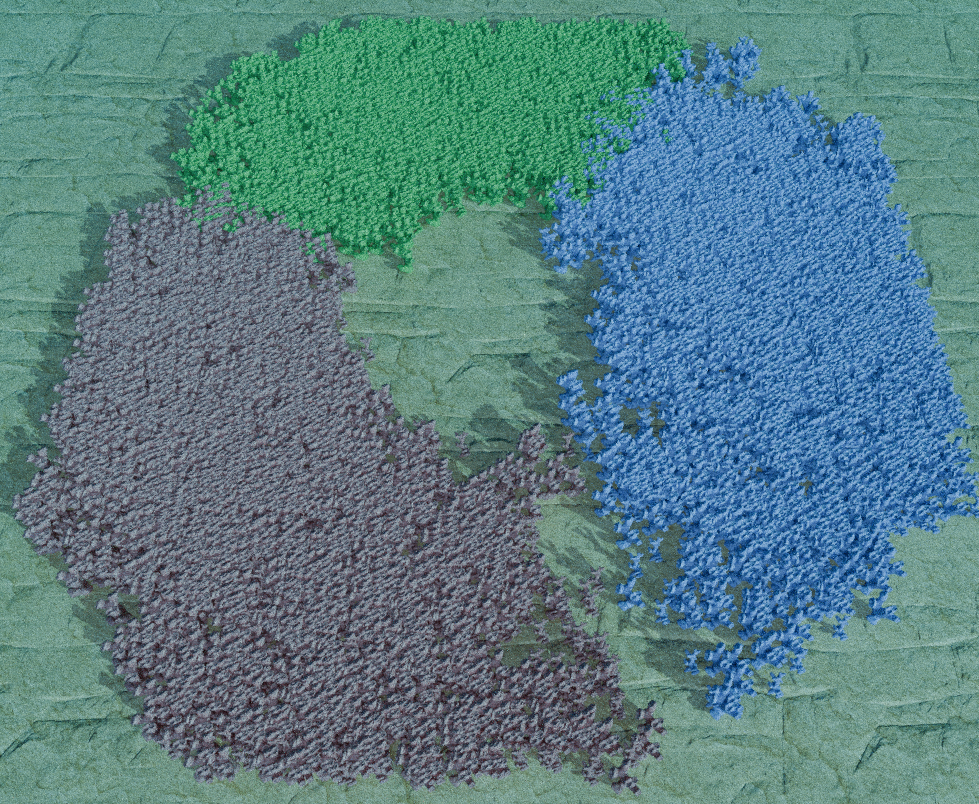
\includegraphics[width=0.24 \linewidth]{col3.png}
    \caption{Three colonies of coral (red, blue, green) restricted to an annulus the middle section of the terrain fighting for the space.}
    \label{fig:env-obj-coral-colonization-scene}
\end{figure*}

\begin{figure*}
    % \centering
    \autofitgraphics[]{Canyon2.png, Canyon3.png, Canyon4.png, Canyon5.png}
    % 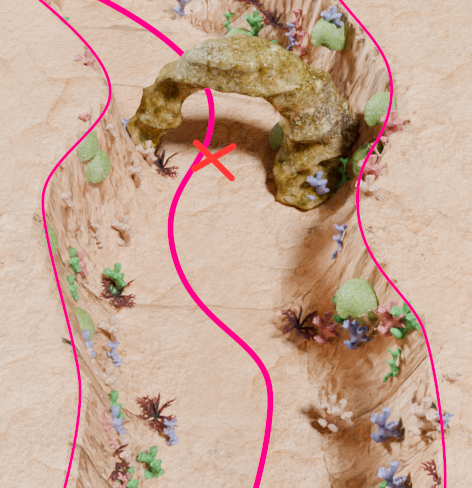
\includegraphics[width = 0.24 \linewidth]{Canyon2.png}
    % 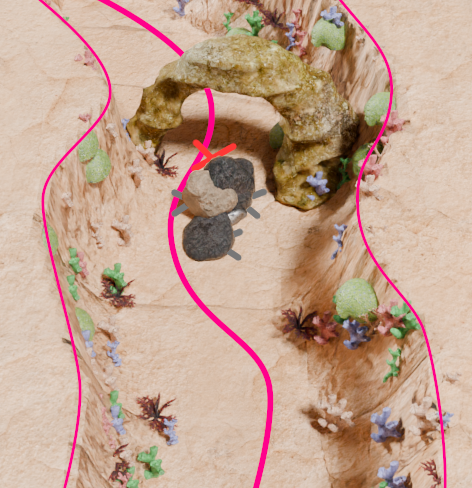
\includegraphics[width = 0.24 \linewidth]{Canyon3.png}
    % 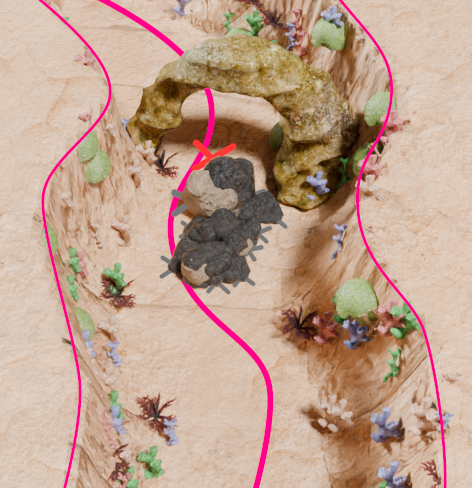
\includegraphics[width = 0.24 \linewidth]{Canyon4.png}
    % 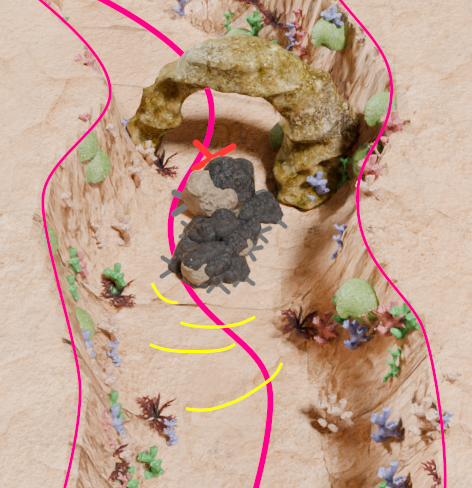
\includegraphics[width = 0.24 \linewidth]{Canyon5.png}
    \caption{Evolution of a canyon scene at different iterations of the simulation. The apparition of an arch causes the spawning of rocks, pebbles, and finally some deposition of sand at the bottom of the canyon, spawning ripples. }
    \label{fig:env-obj-canyon-scene}
\end{figure*}


The proposed method aims to generate plausible landscapes using simplified versions of the evolution of an ecosystem and of the 3D representation. The biological realism of the result is highly correlated to the amount of simplification and assumptions, while the visual realism is completely dependent to the geometric functions used for the 3D modeling of the \glosses{EnvObj}. While proposing a flexible method that propose a generic approach for terrain generation, a close collaboration with fields experts and with graphists is needed to achieve optimal results.

Most simulation algorithm's quality depends on the size of the time step used, but with the introduction of a decay rate in the \glosses{EnvMat} properties, we limit the influence of time steps by considering that steady-state are reachable. The material deposition and absorption on punctual \glosses{EnvObj} can be seen as a Dirac function $\dirac$ centered at their position resulting in the advantage that material displacement function can use the definition of the diffusion equation instead of the advection-diffusion-reaction equation. This equation allowing us to evaluate the state of the material $\material$ without intermediate steps, but this is not applicable with curve- and region-based \glosses{EnvObj}. 

\section{Conclusion}
\label{sec:env-obj-conclusion}
We have proposed a method to generate terrains procedurally using sparse representations. This representation, the \glosses{EnvObj}, enables to introduce expert knowledge by the mean of the \glosses{FitnessFunc} that rule the \glosses{EnvObj} life cycle, but also to integrate the user in the loop during the generation process. We reduced the terrain resolution limitations by defining the environment objects as parametric features. Thanks to the sparse representation based on single points, curves and regions, we allow for direct manipulation of the \glosses{EnvObj} of the scene by the user which, thanks to the environment steady state consideration, also enables to include these interactions in the automatic simulation process.
Integrating environmental properties in the \gloss{FitnessFunc} of \glosses{EnvObj} allows the user to guide the generation through \glosses{GeoEvent}. Our method enables each \gloss{EnvObj} of the scene to influence the environment locally, reducing the need of computations while also retrieving \glosses{EnvVal} locally, which result in a parallelizable life-like simulation process. The genericity of the environment properties definitions should be sufficient for plausible generation of other landscape types as long as expert knowledge can be translated to \gloss{EnvObj}'s formalism.


We limited our work to the use of 2D scalar fields as they are more easily differentiable, interpretable and lighter than volumetric representations. However, future works include using 3D representations of the terrain and the environment to generate 3D terrains, including cavities, sub-terrestrial areas and the interior of coral structures. 
% The different possibilities to explore for this would be: the use of 3D particles to represent the state of the \glosses{EnvMat} in the environment, or voxel grids or flatten representation of the terrain's surface (but would not allow a different morphological shape than the height field...).

\begin{figure}[H]
    % \centering
    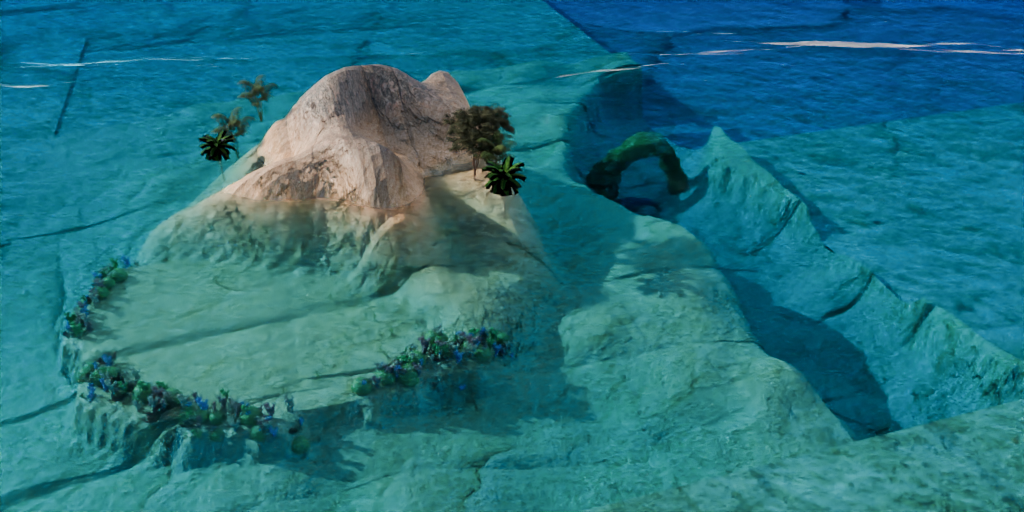
\includegraphics{multiScene1 v2 final 1.png}
    \caption{A simple coral reef island is generated using an island, a lagoon, reefs coral polyps, beaches, trees and algae \glosses{EnvObj}. Trees appear on beaches and algae grow in the lagoon's sand. }
    \label{fig:env-obj-coral-island-scene}
\end{figure}














% \section{Method}
% \label{sec:env-obj-method}
% The overall pipeline of the method is based on simple incremental generation like most rule-based systems. In this type of system, the final state is defined either by reaching equilibrium, or by verifying specific conditions, such as a maximum number of iterations. 
% We define our pipeline in three phases (\cref{fig:env-obj-pipeline}): the initialization phase that describe the generation and simulation rules, the iterative phase generating populating the terrain with our \glosses{EnvObj} and finally the output.


% \subsection{Pipeline overview}





















% \section{Expert knowledge integration}
% \label{sec:env-obj-biology}
%   The definition of the \glosses{FitnessFunc} of the \glosses{EnvObj} are inspired by the biological and geological factors that rule the evolution of underwater landscapes. The main factors are depth, light, water currents and biodiversity. External \glosses{GeoEvent} have direct and indirect repercussions on the biodiversity of underwater environments. Coral reef islands are complex bio systems in which fauna, flora and geology are mixed together. 

% \subsection{\Glosses{EnvObj} description}
% \label{sec:env-obj-represented-objects}
% We have represented with \glosses{EnvObj} some geologic features, animal features and flora features. The low island is most often raised in a circular shape as the process mainly appear around a hot spot under the ground. The evolution of an island into a coral reef island requires that the environmental conditions are sufficient for coral development: corals will grow slightly below the water surface as waves will break its growth and at a shallow depth (around 3m to 30m deep) in order for light to reach it. As coral grow and die, the skeleton is transformed into porous limestone, providing shelter to surrounding animals and reducing the impact of water erosion on the island. Corals drop polyps that are transported by the water flow and when they stick to a hard surface, as a rock or the reef itself, the coral may grow and colonize the area. As subsidence cause the island to lower, the living part of the coral reef keep growing toward light, which lead to a reef that is constantly close to the water level without reaching it due to wave erosion. The survival of reefs depends on the equilibrium between coral growth and and erosion. Eroded parts of the reef falling in the sheltered part of the reef accumulates, ending up by forming a lagoon. An island formed by a hot spot will inevitably subside in time, until it is completely flatten. As the coral reefs keep growing, only the lagoon remain, resulting in an atoll. \\
% In this work we we integrate the biological and geological knowledge in the \glosses{FitnessFunc} of the \glosses{EnvObj} we want to generate. We represent the islands as regions that can be appearing with a uniform distribution. From the formulation of the region description \eqref{eq:internal-energy-equation}, we mostly create circular islands. The coral features, \glosses{EnvObj} described as a single point, have a \gloss{FitnessFunc} that take into account the depth of the ground, the amount of sand, fresh water and polyps in their environment, as well as the strength of water currents. Each coral species have different living conditions, but we reduced our work to soft coral which are sensible to water strength and stony corals that are more resistant to erosion. Reefs are formed as coral's skeleton are transformed into calcareous stone, describing then as an \gloss{EnvObj} representing multiple others. 

% \subsection{Simplifications}
% \label{sec:env-obj-simplifications}
% The environmental factors simulated are greatly simplified as the real processes are in a very small time scale, that computer simulation are not able to simulate in interactive time. The use of \glosses{EnvObj} aim to represent a plausible results, while avoiding modeling the smaller scale \glosses{GeoEvent}. Examples of simplifications are the geometry and material of each \gloss{EnvObj}, which have an influence on the water currents through friction, the water currents represented as stationary flows, while the water flow dynamics are a complex system that may change completely at two different times of the day, the animal influence on the reefs that they transform by the ingestion and deposition of sediments, ...
